\documentclass[10pt, a4paper]{article}
% \usepackage[english]{babel}
\usepackage[brazilian]{babel}
\usepackage[utf8]{inputenc}
% \usepackage[T1]{fontenc}

% matlab code
% \usepackage{matlab-prettifier}
\usepackage[numbered,framed]{matlab-prettifier}
\renewcommand{\lstlistingname}{Anexo} % Listing->Code
\let\ph\mlplaceholder % shorter macro
\definecolor{codegreen}{rgb}{0,0.6,0}
\definecolor{codegray}{rgb}{0.5,0.5,0.5}
\definecolor{codepurple}{rgb}{0.58,0,0.82}
\definecolor{backcolour}{rgb}{0.95,0.95,0.92}
\lstdefinestyle{myStyle}{
    language=Matlab,
    breaklines=true,
    frame=single,
    numbers=none,
    basicstyle=\ttfamily\footnotesize,
%     basicstyle=\footnotesize\ttfamily,
    keywordstyle=\bfseries\color{magenta},
    commentstyle=\color{codegreen},
    identifierstyle=\color{blue},
    backgroundcolor=\color{backcolour},
    stringstyle=\color{codepurple},
}
\usepackage{adjustbox}

% For subfigure use
\usepackage[font=small,labelfont=bf]{caption}
\usepackage{subcaption}

% Set page size and margins
% Replace `letterpaper' with`a4paper' for UK/EU standard size
\usepackage[a4paper,top=2cm,bottom=2cm,left=2cm,right=2cm,marginparwidth=2cm]{geometry}

% tabelas
\usepackage{array}
\usepackage{tabularx}
\usepackage{booktabs}

\usepackage{float}

% Useful packages
\usepackage{amsmath}

\usepackage{graphicx}
\graphicspath{{figures/}} %Setting the graphicspath
\usepackage[colorlinks=true, allcolors=blue]{hyperref}

% \title{PUC-RJ Pontif\'icia Universidade Cat\'olica do Rio de Janeiro \\ MEC 2403 - Otimiza\c c\~ao e Algoritmos para Engenhria Mec\^anica \\ Trabalho 01 - Otimiza\c c\~ao  sem Restri\c c\~oes  \\
% \large Professor: Ivan Menezes}

% \author{Felipe da Costa Pereira - mat. 2212376 \\ {\tt felipecostapereira@gmail.com}}

\begin{document}

\begin{titlepage}
      \begin{center}
          \vspace*{1cm}

          \Huge
          \textbf{Trabalho 01 \\ Otimiza\c c\~ao  sem Restri\c c\~oes}

          \vspace{0.5cm}
          \LARGE
          MEC 2403 - Otimiza\c c\~ao e Algoritmos para Engenhria Mec\^anica

          \vspace{1.5cm}

          \textbf{Felipe da Costa Pereira \\ {\tt felipecostapereira@gmail.com}}

          \vfill
          Professor: Ivan Menezes

          \vspace{0.8cm}

          
\includegraphics[width=0.2\textwidth]{puc.jpg}

          \Large
          Departamento de Engenharia Mec\^anica\\
          PUC-RJ Pontif\'icia Universidade Cat\'olica do Rio de Janeiro\\
          outubro, 2022

      \end{center}
  \end{titlepage}

% \maketitle

\section{Introdu\c c\~ao}

Otimiza\c c\~ao sem restri\c c\~ao (OSR) consiste em encontrar o m\'inimo de uma fun\c c\~ao $f(\vec{x})$ onde n\~ao h\'a restri\c c\~ao em rela\c c\~ao ao dom\'inio das vari\'aveis $\vec{x}$. A fim de se encontrar o minimo da fun\c c\~ao $f(\vec{x})$ a partir de um ponto de partida $(\vec{x_{0}})$ , os m\'etodos apresentados nesse trabalho consistem na repeti\c c\~ao das etapas seguintes at\'e que um crit\'erio de parada seja atingido:
\begin{enumerate}
      \item Selecionar uma dire\c c\~ao $\vec{d}$ a partir do ponto $\vec{x_{0}}$
      \item Encontrar o m\'inimo da fun\c c\~ao $f$ nessa dire\c c\~ao, chegando a um novo ponto $\vec{x_{1}} = \vec{x_{0}} + \alpha\vec{d}$, onde $\alpha$ \'e um n\'umero real (busca linear).
      \item Tomar $\vec{x_{1}}$ como o novo ponto de partida $\vec{x_{0}}$
      \item Repetir os passos de 1 a 3 at\'e que uma condi\c c\~ao de parada seja atingida: m\'inimo encontrado ($|\vec{\nabla f}|=0$), ou m\'aximo n\'umero de itera\c c\~oes atingido.
\end{enumerate}

A etapa descrita no item 2 consiste na minimiza\c c\~ao de uma fun\c c\~ao de uma \'unica vari\'avel ($\alpha$). Dessa forma o problema de minimiza\c c\~ao da fun\c c\~ao $f(\vec{x})$ se torna um problema de sucessivas determina\c c\~oes de dire\c c\~oes de busca e suas respectivas buscas lineares nessas dire\c c\~oes.

\section{Objetivos}

Os principais objetivos deste trabalho s\~ao:
\begin{itemize}
      \item Implementar numericamente os algoritmos de otimiza\c c\~ao: Univariante, Powell, Steepest Descent, Fletcher-Reeves, Newton-Raphson e BFGS.
      \item Avaliar a influ\^encia dos par\^ametros dos algoritmos nas m\'etricas de converg\^encia e comparar essas \'ulltimas com os valores esperados da teoria.
      \item Aplicar os algoritmos implementados na solu\c c\~ao do problema de OSR em tr\^es casos: uma fun\c c\~ao quadr\'atica, uma n\~ao quadr\'atica e uma terceira fun\c c\~ao que representa um problema de engenharia (minimizaz\c c\~ao da energia de um sistema massa-mola visando encontrar seu ponto de equil\'ibrio est\'atico)
\end{itemize}

As fun\c c\~oes a serem minimizadas neste trabalho s\~ao: \\
\\
Problema 01a):
\begin{equation}\label{fun:01a}\tag{1a}
      f(x_{1},x_{2})=x_{1}^2 - 3x_{1}x_{2} + 4x_{2}^2 + x_{1} - x_{2}
\end{equation}
a partir dos pontos iniciais $x^0=\{2,2\}^t$ e $x^0=\{-1,-3\}^t$
\\ \\
Problema 01b):
\begin{equation}\label{fun:01b}\tag{1b}
f(x_{1},x_{2}) = (1+a-bx_{1}-bx_{2})^2 + (b+x_{1}+ax_{2} - bx_{1}x_{2})^2
\end{equation}
com $a=10$ e $b=1$ a partir dos pontos iniciais $x^0=\{10,2\}^t$ e $x^0=\{-2,-3\}^t$
\\ \\
Problema 02:
\begin{equation}\label{fun:02}\tag{2}
\Pi(x_{1},x_{2})= 450(\sqrt{(30+x_{1})^2+x_{2}^2}-30)^2 + 300(\sqrt{(30-x_{1})^2+x_{2}^2}-30)^2 -360x_{2}
\end{equation}
a partir dos ponto inicial $x^0=\{0.01,-0.10\}^t$


\section{Algoritmos de Busca Linear}

Os algoritmos de minimiza\c c\~ao s\~ao executados em duas etapas conforme citado anteriormente: a primeira etapa consiste em determinar uma dire\c c\~ao de busca $\vec{d}$ e em seguida promove-se a minimiza\c c\~ao da fun\c c\~ao $f$ nessa dire\c c\~ao, o que significa encontrar o valor de  $\alpha=\alpha_{k}$ que minimiza a fun\c c\~ao $f(x=x_{0}+\alpha\vec{d})$ ao longo da dire\c c\~ao $\vec{d}$. A partir do valor de $\alpha_{k}$ encontra-se um novo ponto de partida $f(x_{k+1}=x_{k}+\alpha_{k}\vec{d_{k}})$. Uma nova dire\c c\~ao $\vec{d_{k+1}}$ \'e ent\~ao determinada e o processo se repete at\'e que uma condi\c c\~ao de parada seja atingida.

Neste trabalho, a busca linear \'e relizada em duas etapas: Passo constante e refinamento do c\'alculo de $\alpha$ atrav\'es do m\'etodo da se\c c\~ao \'aurea.

Um maior detalhamento dos m\'etodos de busca aqui apresentados, assim como outros comumente utilizados na solu\c c\~ao de problemas de otimiza\c c\~ao pode ser encontrado em \cite{apostila}.

\subsection{Passo Constante}

A primeira etapa da busca linear consiste numa busca inexata que visa encontrar um intervalo de valores do passo $\alpha$, $[\alpha_{L}, \alpha_{H}]$ que represente uma redu\c c\~ao suficientemente grande da fun\c c\~ao $f$. Essa implementa\c c\~ao num\'erica incrementa o passo de um valor $d\alpha$ at\'e que a fun\c c\~ao pare de diminuir.

\subsection{Bisse\c c\~ao e Se\c c\~ao \'Aurea}

Ap\'os a etapa do passo constante, os m\'etodos da Bisse\c c\~ao ou Se\c c\~ao \'Aurea s\~ao aplicados para encontrar o valor de $\alpha$, entre os valores determinados no intervalo da etapa 1. Em ambos os casos, o intervalo de ocorr\^encia do valor m\'inimo de $f$ \'e sucessivamente reduzido at\'e que seja muito pequeno e considera-se, dado esse crit\'erio num\'erico, solucionado o problema da minimiza\c c\~ao de $f$ nessa dire\c c\~ao, encontrando o passo $\alpha_{k}$ correspondente a esse m\'inimo.

O m\'etodo da bisse\c c\~ao divide sucessivamente o intervalo descartando a parte superior ou inferior do mesmo avaliando o valor da fun\c c\~ao $f$ na vizinhan\c ca esquerda e direita de um $\alpha_{M}$ m\'edio do intervalo. J\'a o m\'etodo da se\c c\~ao \'aurea utiliza a raz\~ao \'aurea para descarte dos intervalos onde $f$ aumenta. Este \'ultimo m\'etodo realiza mais passos, por\'em possui a vantagem de avaliar menos vezes a fun\c c\~ao $f$ uma vez que os valores avaliados no passo anterior podem ser reutilizados no passo seguinte do algoritmo, o que pode ser interessante em problemas onde a avalia\c c\~ao da fun\c c\~ao $f$ \'e computacionalmente cara.

\section{Algoritmos de Dire\c c\~ao}

Conforme descrito anteriormtente, os m\'etodos de dire\c c\~ao determinam dire\c c\~oes de busca do m\'inimo de $f$ a partir de um ponto $\vec{x_{k}}$. A partir da busca linear encontra-se o valor do passo nessa dire\c c\~ao que minimiza $f$, ($\alpha_{k}$), os algoritmos de dire\c c\~ao calculam, ent\~ao, a pr\'oxima dire\c c\~ao onde se deve minimizar $f$ e a partir do novo ponto $\vec{x_{k+1}}=\vec{x_k}+\alpha_{k}\vec{d}$.

Os algoritmos de determina\c c\~ao das dire\c c\~oes de busca utilizados nesse trabalho s\~ao brevemente descritos a seguir.

Um maior detalhamento dos algortimos de dire\c c\~ao aqui apresentados, assim como outros comumente utilizados na solu\c c\~ao de problemas de otimiza\c c\~ao pode ser encontrado em \cite{apostila}.


\subsection{Univariante}

O m\'etodo univariante \'e o mais simples, onde as dire\c c\~oes de busca s\~ao as dire\c c\~oes can\^onicas, $\vec{d_{k}}=\vec{e_{k}}$. Esse procedimento \'e equivalente a modificar uma vari\'avel de cada vez no processo iterativo, ou seja, apenas a vari\'avel na posi\c c\~ao $k$ do vetor de vari\'aveis $\vec{x}$ \'e modificada na itera\c c\~ao $k$ (\cite{apostila})
\subsection{Powell}

O m\'etodo de Powell utiliza em seu algoritmo dire\c c\~oes denominadas "movimento padr\~ao". O m\'etodo de Powell gera dire\c c\~es Q-conjugadas, o que representa uma acelera\c c\~ao em rela\c c\~ao ao m\'etodo univariante. Um maior detalhamento sobre o m\'etod de Powell e a demonstra\c c\~ao de que o m\'etodo de Powell converge para o m\'inimo de uma fun\c c\~ao quadr\'atica de $n$ vari\'aveis em um n\'umero finito de passos dado por $n+1$ est\'a descrito em (\cite{apostila}).

\subsection{Steepest Descent}

O m\'etdo Steepest Descent \'e um m\'etodo onde as dire\c c\~oes s\~ao dadas pela dire\c c\~ao oposta ao gradiente da fun\c c\~ao $f$. Ou seja, $\vec{d_{k}} = -\vec{\nabla} f(\vec{x_{k}})$.

\subsection{Fletcher-Reeves}

Este m\'etodo consiste em uma adapta\c c\~ao do m\'etodo dos Gradientes Conjugados que o torna capaz de ser usado para minimiza\c c\~ao de uma fun\c c\~ao qualquer. Para anto, duas modifica\c c\~oes precisam ser realizadas, a avaliacao da matriz Q (ou Hessiana para funcao nao quadratica) \'e substituida por uma busca linear e o parametro $\beta$ modificado (\cite{apostila}).

\subsection{Newton-Raphson}

O princ\'ipio deste m\'etodo \'e minimizar uma fun\c c\~ao $f$ atrav\'es de uma aproxima\c c\~ao local por uma fun\c c\~ao quadr\'atica. A dire\c c\~ao de minimiza\c c\~ao de $f$ \'e obtida a partir da derivada da expans\~ao de $f$ numa s\'erie de Taylor de ordem 2 em rela\c c\~ao a $\vec{d_{k}}$, de onde se obt\'em: $\vec{d_{k}}=-H^{-1} \vec{\nabla} f(\vec{x_{k}})$, onde H \'e a matriz Hessiana da fun\c c\~ao $f$ (\cite{apostila}).

\subsection{BFGS}

O m\'etodo Broyden-Fletcher-Goldfarb-Shanno (BFGS) \'e um m\'etodo para resolver um problema de otimiza\c c\~ao n\~ao linear sem restri\c c\~oes. trata-se de uma solu\c c\~ao frequentemente usada quando se deseja um algoritmo com dire\c c\~oes de descida.

A ideia principal deste m\'etodo \'e evitar a constru\c c\~ao expl\'icita da matriz Hessiana e, em vez disso, construir uma aproxima\c c\~ao da inversa da segunda derivada da fun\c c\~ao a ser minimizada, analisando os diferentes gradientes sucessivos. Esta aproxima\c c\~ao das derivadas da fun\c c\~ao leva a um m\'etodo quase\-Newton (uma variante do m\'etodo de Newton) para encontrar a dire\c c\~ao de busca. A matriz Hessiana n\~ao precisa ser recalculada a cada itera\c c\~ao do algoritmo. No entanto, o m\'etodo assume que a fun\c c\~ao pode ser aproximada localmente por uma expans\~ao quadr\'atica limitada em torno do \'otimo (\cite{bfgs}).

\section{Metodologia}

Para atingir os objetivos do trabalho, foram programados scripts em linguagem Matlab, organizados conforme esquematizado na figura \ref{fig:fluxo}.

\begin{figure}[H]
      \centering
      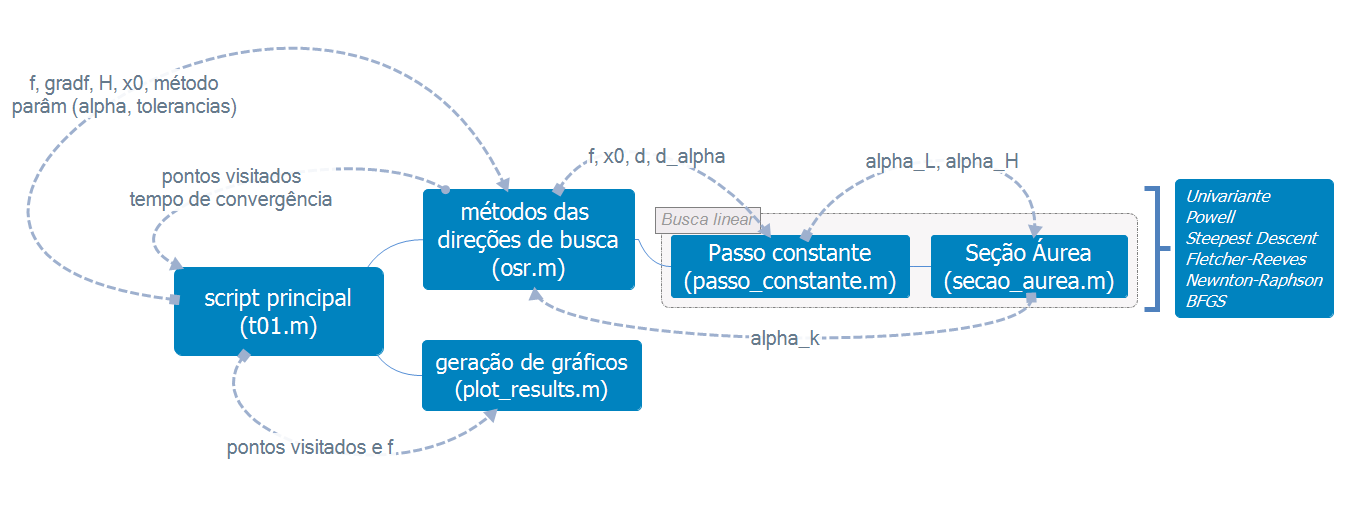
\includegraphics[width=.9\textwidth]{t01.png}
      \caption{Fluxo dos scripts}
      \label{fig:fluxo}
\end{figure}

Um script principal \textit{t01.m} escolhe os par\^ametros do algoritmo: $a=d\alpha$ (passo da busca linear), m\'aximo n\'umero de itera\c c\~oes (iter\_max) e toler\^ancias para avaliar a converg\^encia da fun\c c\~ao para um m\'inimo ou da se\c c\~ao \'aurea: TOL e TOL2, respectivamente. Al\'em disso esse script cria as fun\c c\~oes, seus gradientes, matriz Hessiana e pontos iniciais, a serem passados como par\^ametros para o script que implementa os algoritmos, conforme ilustrado no anexo \ref{l1}.

Em seguida, o script \textit{t01.m} chama o script \textit{osr.m} (anexo \ref{l2}) para cada m\'etodo e plota as curvas de n\'ivel da fun\c c\~ao $f$ e todos os pontos visitados durante a busca do algoritmo atrav\'es do script \textit{plot\_result.m}

O script \textit{osr.m} implementa de fato os algoritmos a partir dos par\^ametros recebidos, retornando todos os valores de $\vec{x}$ visitados e o tempo de execu\c c\~ao, conforme o anexo \ref{list_osr}.

Outros dois scripts invocados na solu\c c\~ao dos problemas propostos s\~ao \textit{passo\_constante.m} e \textit{secao\_aurea.m}, que realizam a etapa de busca linear para cada dire\c c\~ao de busca. Esses c\'odigos encontram-se nos anexos \ref{list_passo_constante} e \ref{list_secao_aurea}, respectivamente. O script \textit{plot\_result.m} \'e listado no anexo \ref{list_plot_result}.

\section{Resultados}

Visando a converg\^encia de todos os m\'etodos, foram testados alguns valores dos par\^ametros dos algoritmos. A melhor combina\c c\~ao dos par\^ametros, para as fun\c c\~oes dos problemas 1 e 2 em termos de converg\~encia dos algoritmos est\'a listada na tabela \ref{table:params}.

\begin{table}[H]
      \small
      \centering
      \caption{Melhores par\^ametros para converg\^encia dos algoritmos}
      \begin{tabular}{c|c|c|c|c}
                        & $d\alpha$ & TOL(gradiente) & TOL2(busca linear) & max\_iter \\
            \hline
            Problema 01 & 0.002 & 1e-4 & 1e-7 & 100 \\
            Problema 02 & 0.005 & 5e-4 & 1e-7 & 100 \\
      \end{tabular}
      \label{table:params}
\end{table}

As tabelas \ref{table:resultadosf1a}, \ref{table:resultadosf1b} apresentam os principais resultados dos algoritmos implementados para as fun\c c\~oes dos itens \ref{fun:01a} e \ref{fun:01b}. Al\'em dos pontos de m\'inimo encontrado, as tabelas apresentam tamb\'em o n\'umero de passos para a converg\^encia e o tempo de execu\c c\~ao.

\begin{table}[H]
      \small
      \centering
      \caption{Resultados para a fun\c c\~ao \ref{fun:01a}}
      \begin{tabular}{c|c|c|c|c}
            m\'etodo           & $x^0$ & $x^{min}$ & passos & $\Delta t$(ms) \\
            \hline
            Univariante         & $\{2,2\}^t$     & $\{-0.7142,-0.1428\}^t$  & 34 & 4.8 \\
            Univariante         & $\{-1,-3\}^t$   & $\{-0.7144,-0.1429\}^t$  & 36 & 6.9 \\
            \hline
            Powell              & $\{2,2\}^t$     & $\{-0.7143,-0.1429\}^t$  &  6 & 24.8 \\
            Powell              & $\{-1,-3\}^t$   & $\{-0.7143,-0.1429\}^t$  & 12 & 7.2 \\
            \hline
            Steepest Descent    & $\{2,2\}^t$     & $\{-0.7142,-0.1428\}^t$  & 25 & 6.5 \\
            Steepest Descent    & $\{-1,-3\}^t$   & $\{-0.7143,-0.1429\}^t$  &  7 & 3.0 \\
            \hline
            Flecher-Reeves     & $\{2,2\}^t$     & $\{-0.7143,-0.1429\}^t$  &  2 & 2.5 \\
            Flecher-Reeves     & $\{-1,-3\}^t$   & $\{-0.7143,-0.1429\}^t$  &  2 & 1.7 \\
            \hline
            Newton-Raphson     & $\{2,2\}^t$     & $\{-0.7143,-0.1429\}^t$  &  1 & 2.5 \\
            Newton-Raphson     & $\{-1,-3\}^t$   & $\{-0.7143,-0.1429\}^t$  &  1 & 1.1 \\
            \hline
            BFGS                & $\{2,2\}^t$     & $\{-0.7143,-0.1429\}^t$  &  2 & 2.2 \\
            BFGS                & $\{-1,-3\}^t$   & $\{-0.7143,-0.1429\}^t$  &  2 & 1.5 \\
      \end{tabular}
      \label{table:resultadosf1a}
\end{table}

No caso da fun\c c\~ao do item \ref{fun:01a}, o m\'etodo de Powell levou mais passos do que o esperado em teoria para uma fun\c c\~ao quadr\'atica, j\'a que nesse caso \'e esperado que o mesmo atinja a converg\~encia em at\'e 9 passos.

\begin{table}[H]
      \small
      \centering
      \caption{Resultados para a fun\c c\~ao \ref{fun:01b}}
      \begin{tabular}{c|c|c|c|c|c}
            m\'etodo           & $x^0$ & $x^{min}$ & passos & $\Delta t$(ms) \\
            \hline
            Univariante         & $\{10,2\}^t$    & $\{13.0000,4.0000\}^t$  & 45 & 9.9 \\
            Univariante         & $\{-2,-3\}^t$   & $\{7,-2\}^t$  & 45 & 10.8 \\
            \hline
            Powell              & $\{10,2\}^t$    & $\{13.0000,4.0000\}^t$  & 24 & 11.6 \\
            Powell              & $\{-2,-3\}^t$   & $\{7,-2\}^t$  & 18 & 8.0 \\
            \hline
            Steepest Descent    & $\{10,2\}^t$    & $\{13.0000,4.0000\}^t$  & 46 & 2.3 \\
            Steepest Descent    & $\{-2,-3\}^t$   & $\{7,-2\}^t$  & 59 & 2.6 \\
            \hline
            Flecher-Reeves     & $\{10,2\}^t$    & $\{13.0000,4.0000\}^t$  & 41 & 1.6 \\
            Flecher-Reeves     & $\{-2,-3\}^t$   & $\{7,-2\}^t$  & 16 & 0.9 \\
            \hline
            Newton-Raphson(*)   & $\{10,2\}^t$    & $\{10,1\}^t$  &  1 & 0.9 \\
            Newton-Raphson     & $\{-2,-3\}^t$   & $\{12.9999,4.0001\}^t$  &  6 & 4.1 \\
            \hline
            BFGS                & $\{10,2\}^t$    & $\{13.0000,4.0000\}^t$  &  7 & 4.1 \\
            BFGS                & $\{-2,-3\}^t$   & $\{7,-2\}^t$  &  6 & 5.7 \\
      \end{tabular}
      \label{table:resultadosf1b}
\end{table}

No caso da fun\c c\~ao do item \ref{fun:01b} nota-se que o m\'etodo de Newton-Raphson n\~ao convegiu para o primeiro ponto (*). Na verdade o algoritmo parou no crit\'erio de norma do gradiente no primeiro passo, o que leva a uma converg\^encia para um valor equivocado. De fato a busca linear nesse caso retornou um valor tal que, ao final do primeiro passo o algoritmo caiu num ponto o gradiente de $f$ \'e muito pequeno. Tal problema pode ser visualizado tamb\'em graficamente na figura \ref{fig:graf01B_m05}.


As figuras de \ref{fig:graf01_m01} a \ref{fig:graf01_m06} a seguir ilustram as curvas de n\'ivel de $f$ para os casos das fun\c c\~oes dos itens \ref{fun:01a} e \ref{fun:01b}, bem como a trajet\'oria dos pontos $\vec{x_{k}}$ associadoas ao algoritmo de minimiza\c c\~ao.

\begin{figure}[H]
      \centering
      \begin{subfigure}{0.45\textwidth}
            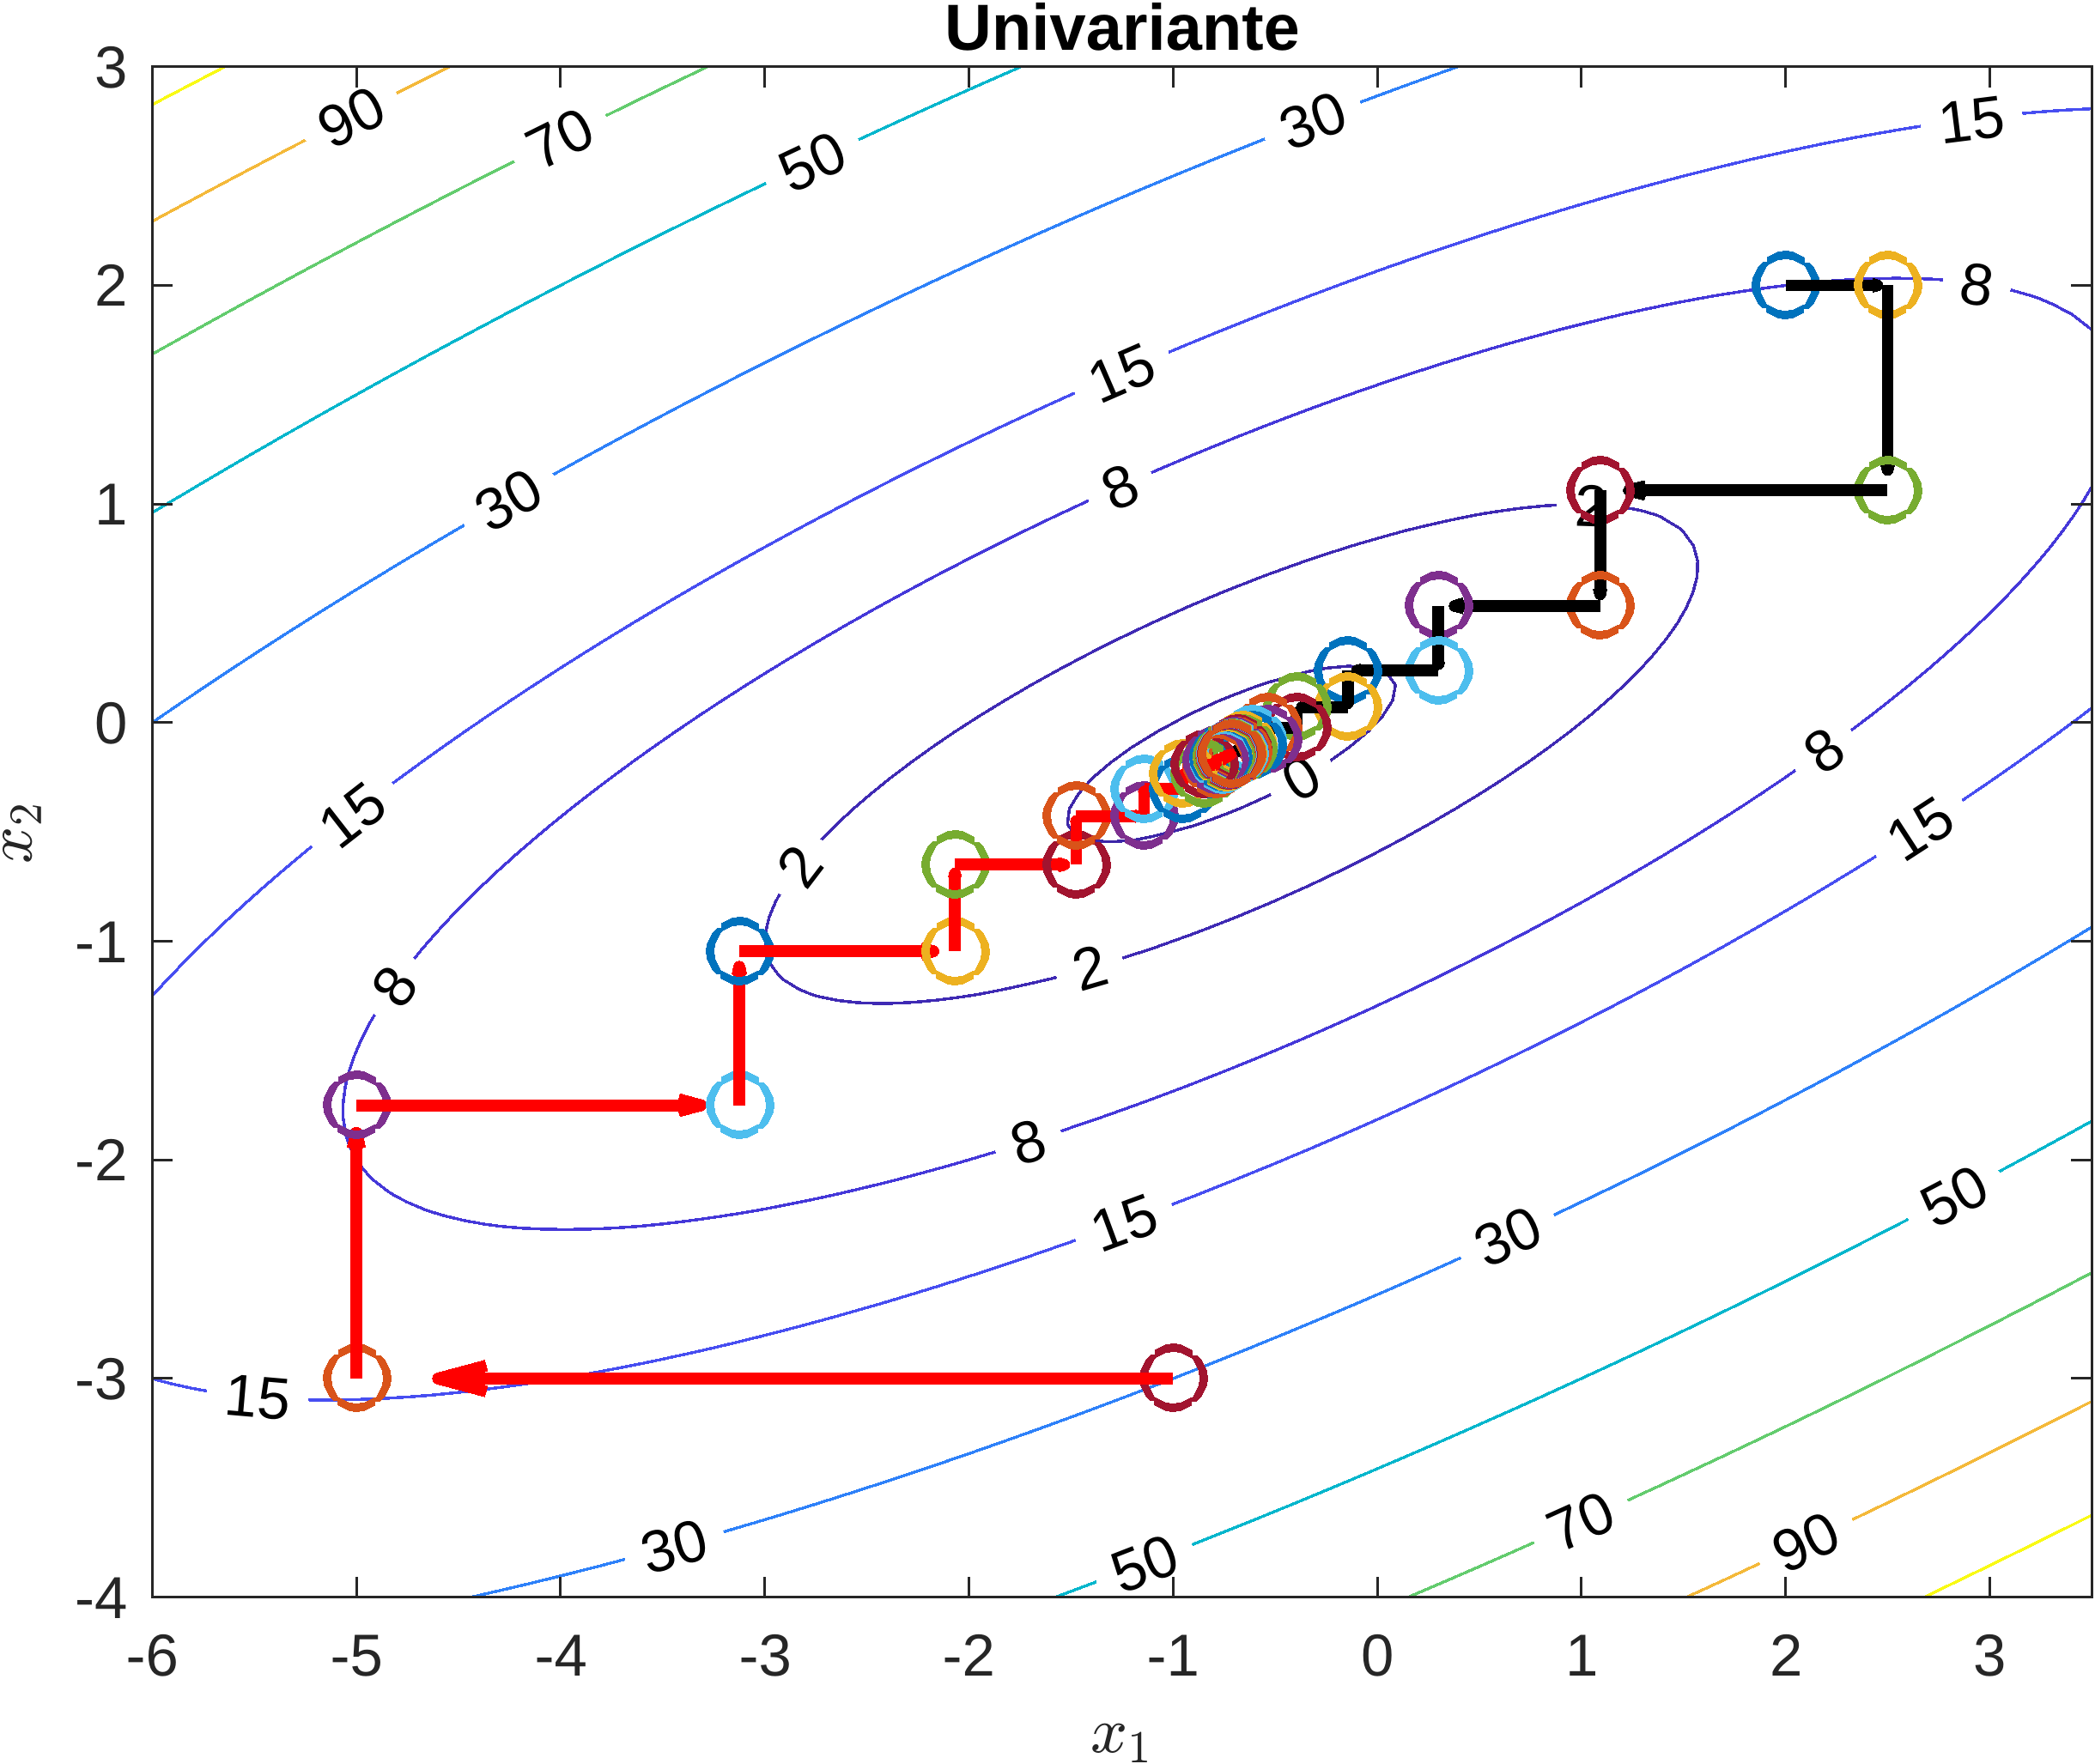
\includegraphics[width=\textwidth]{img01A_m01.png}
            \caption{Curvas de n\'ivel de $f_{1a}$ e pontos $x_{k}$}
            \label{fig:graf01A_m01}
      \end{subfigure}
      \begin{subfigure}{0.45\textwidth}
            \centering
            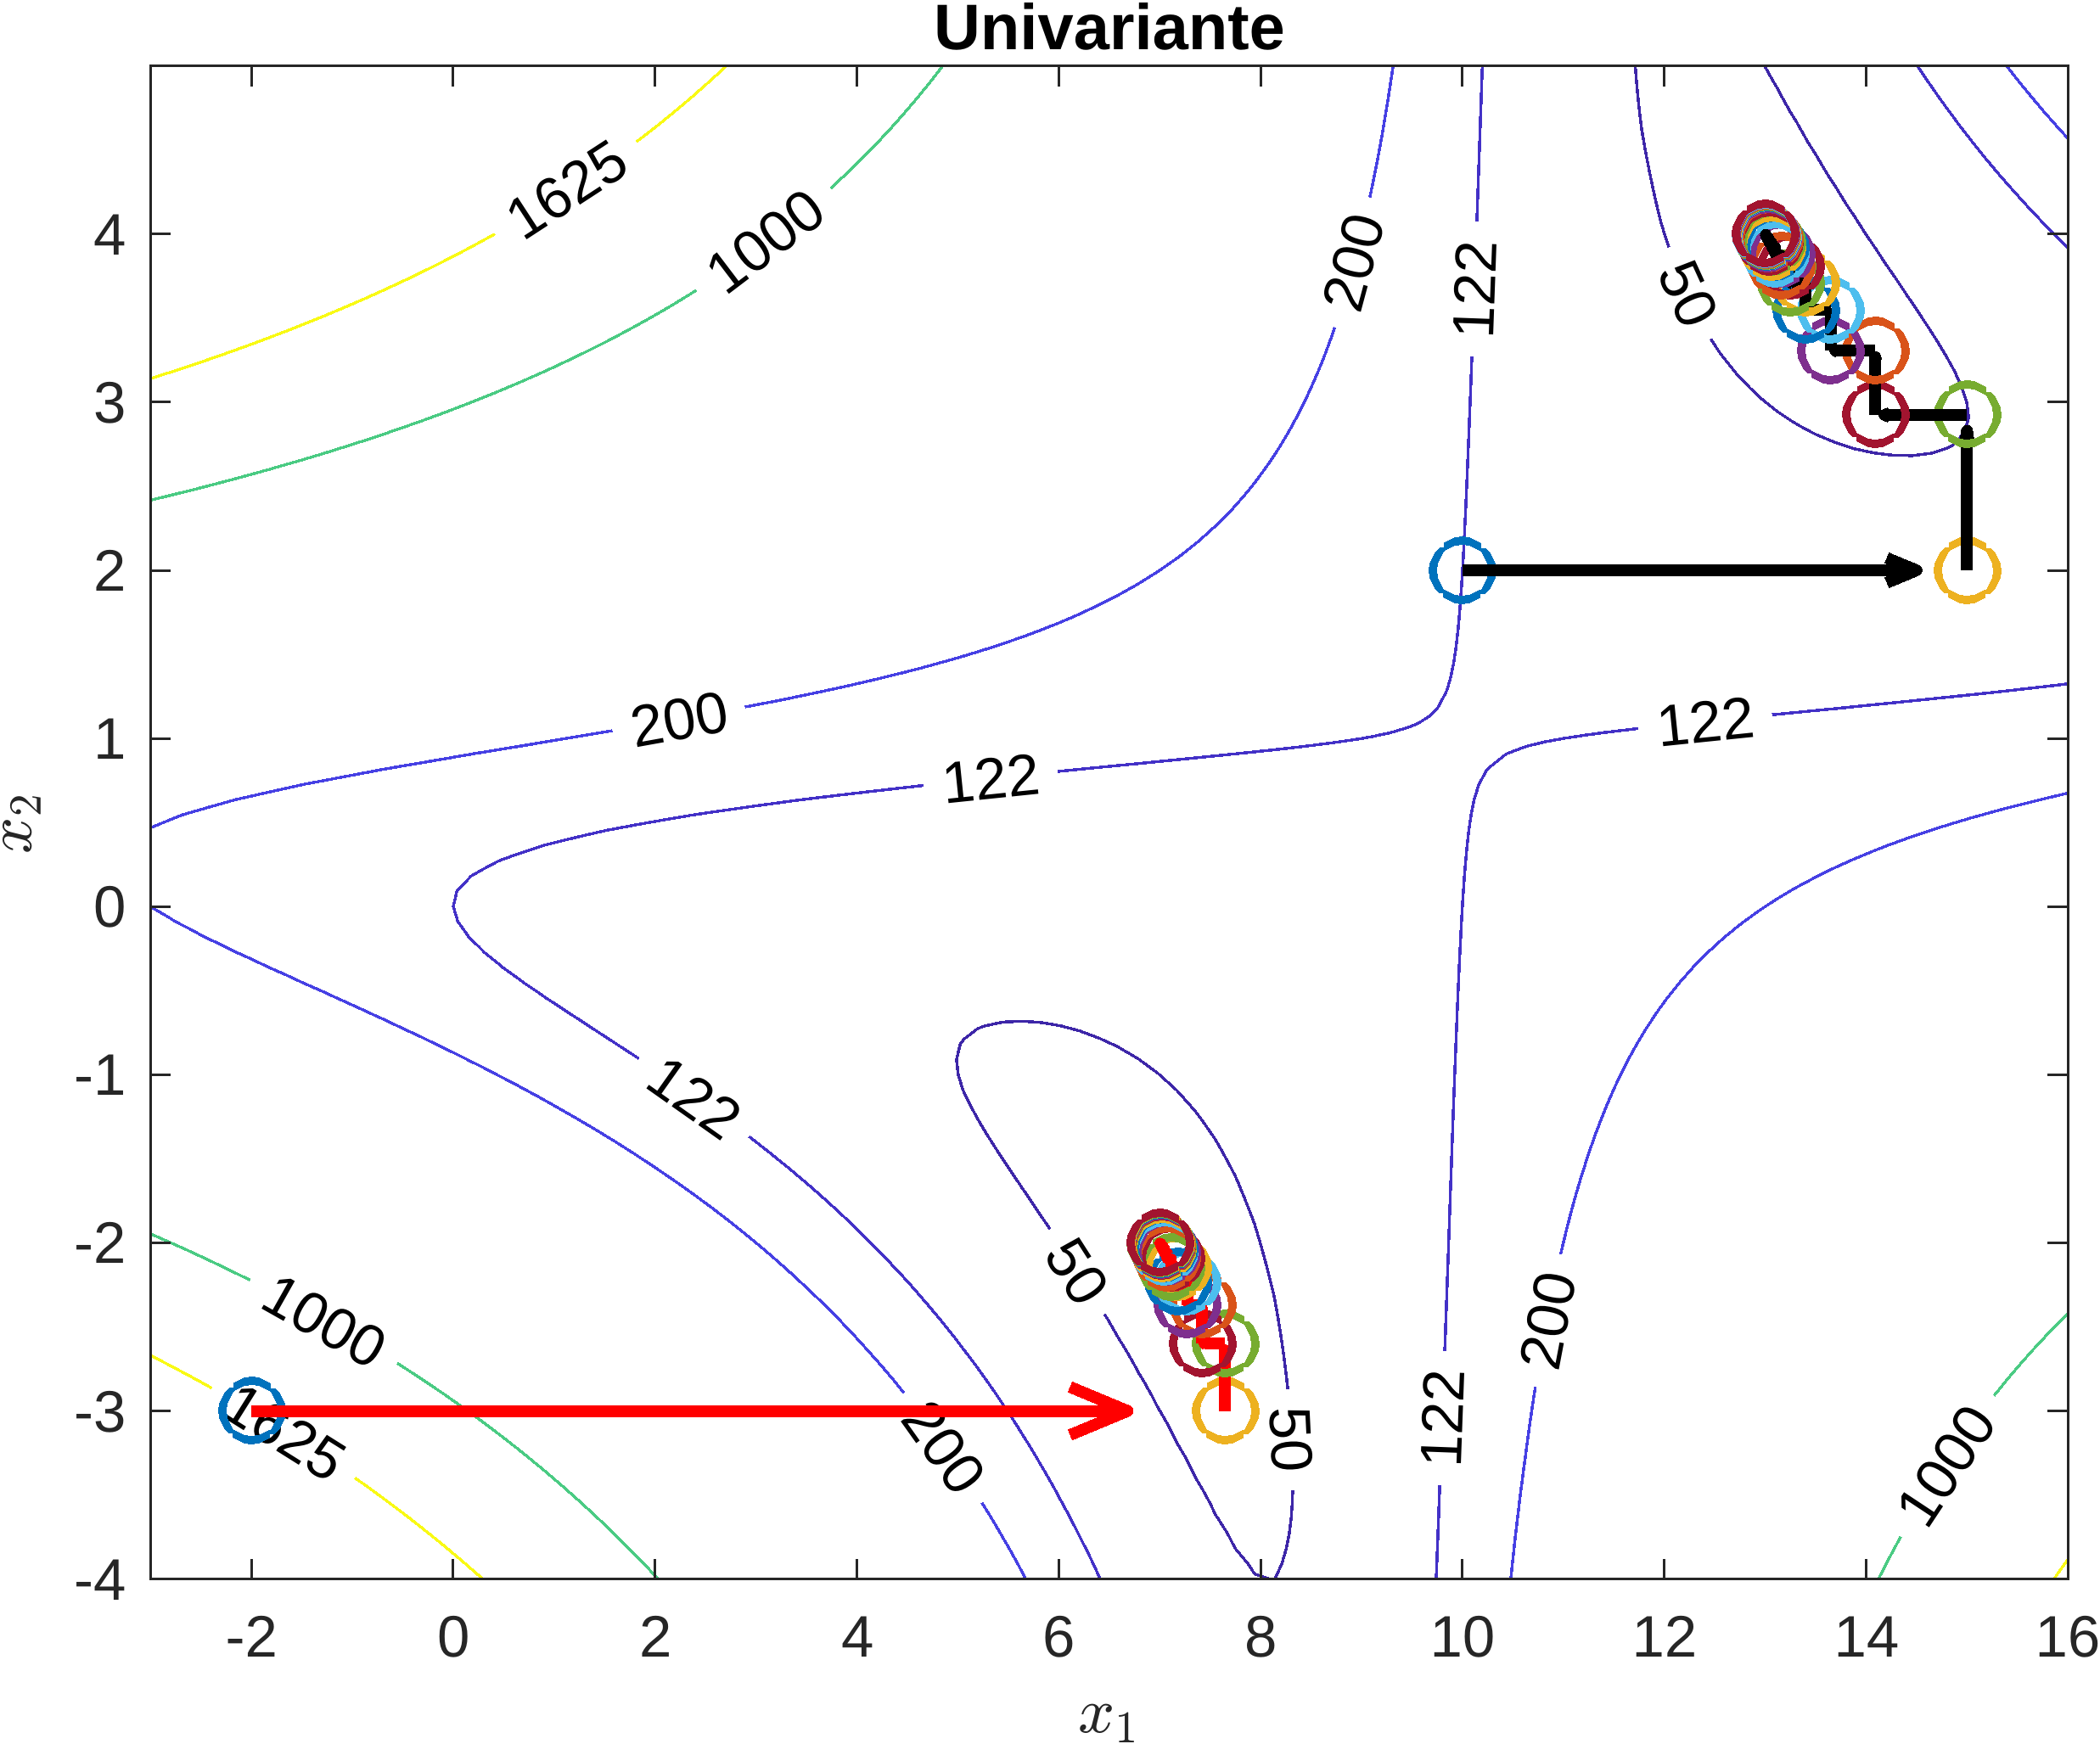
\includegraphics[width=\textwidth]{img01B_m01.png}
            \caption{Curvas de n\'ivel de $f_{1b}$ e pontos $x_{k}$}
            \label{fig:graf01B_m01}
      \end{subfigure}
      \caption{Resultados do m\'etodo univariante, para as duas fun\c c\~oes e pontos iniciais}
      \label{fig:graf01_m01}
\end{figure}

\begin{figure}[H]
      \centering
      \begin{subfigure}{0.45\textwidth}
            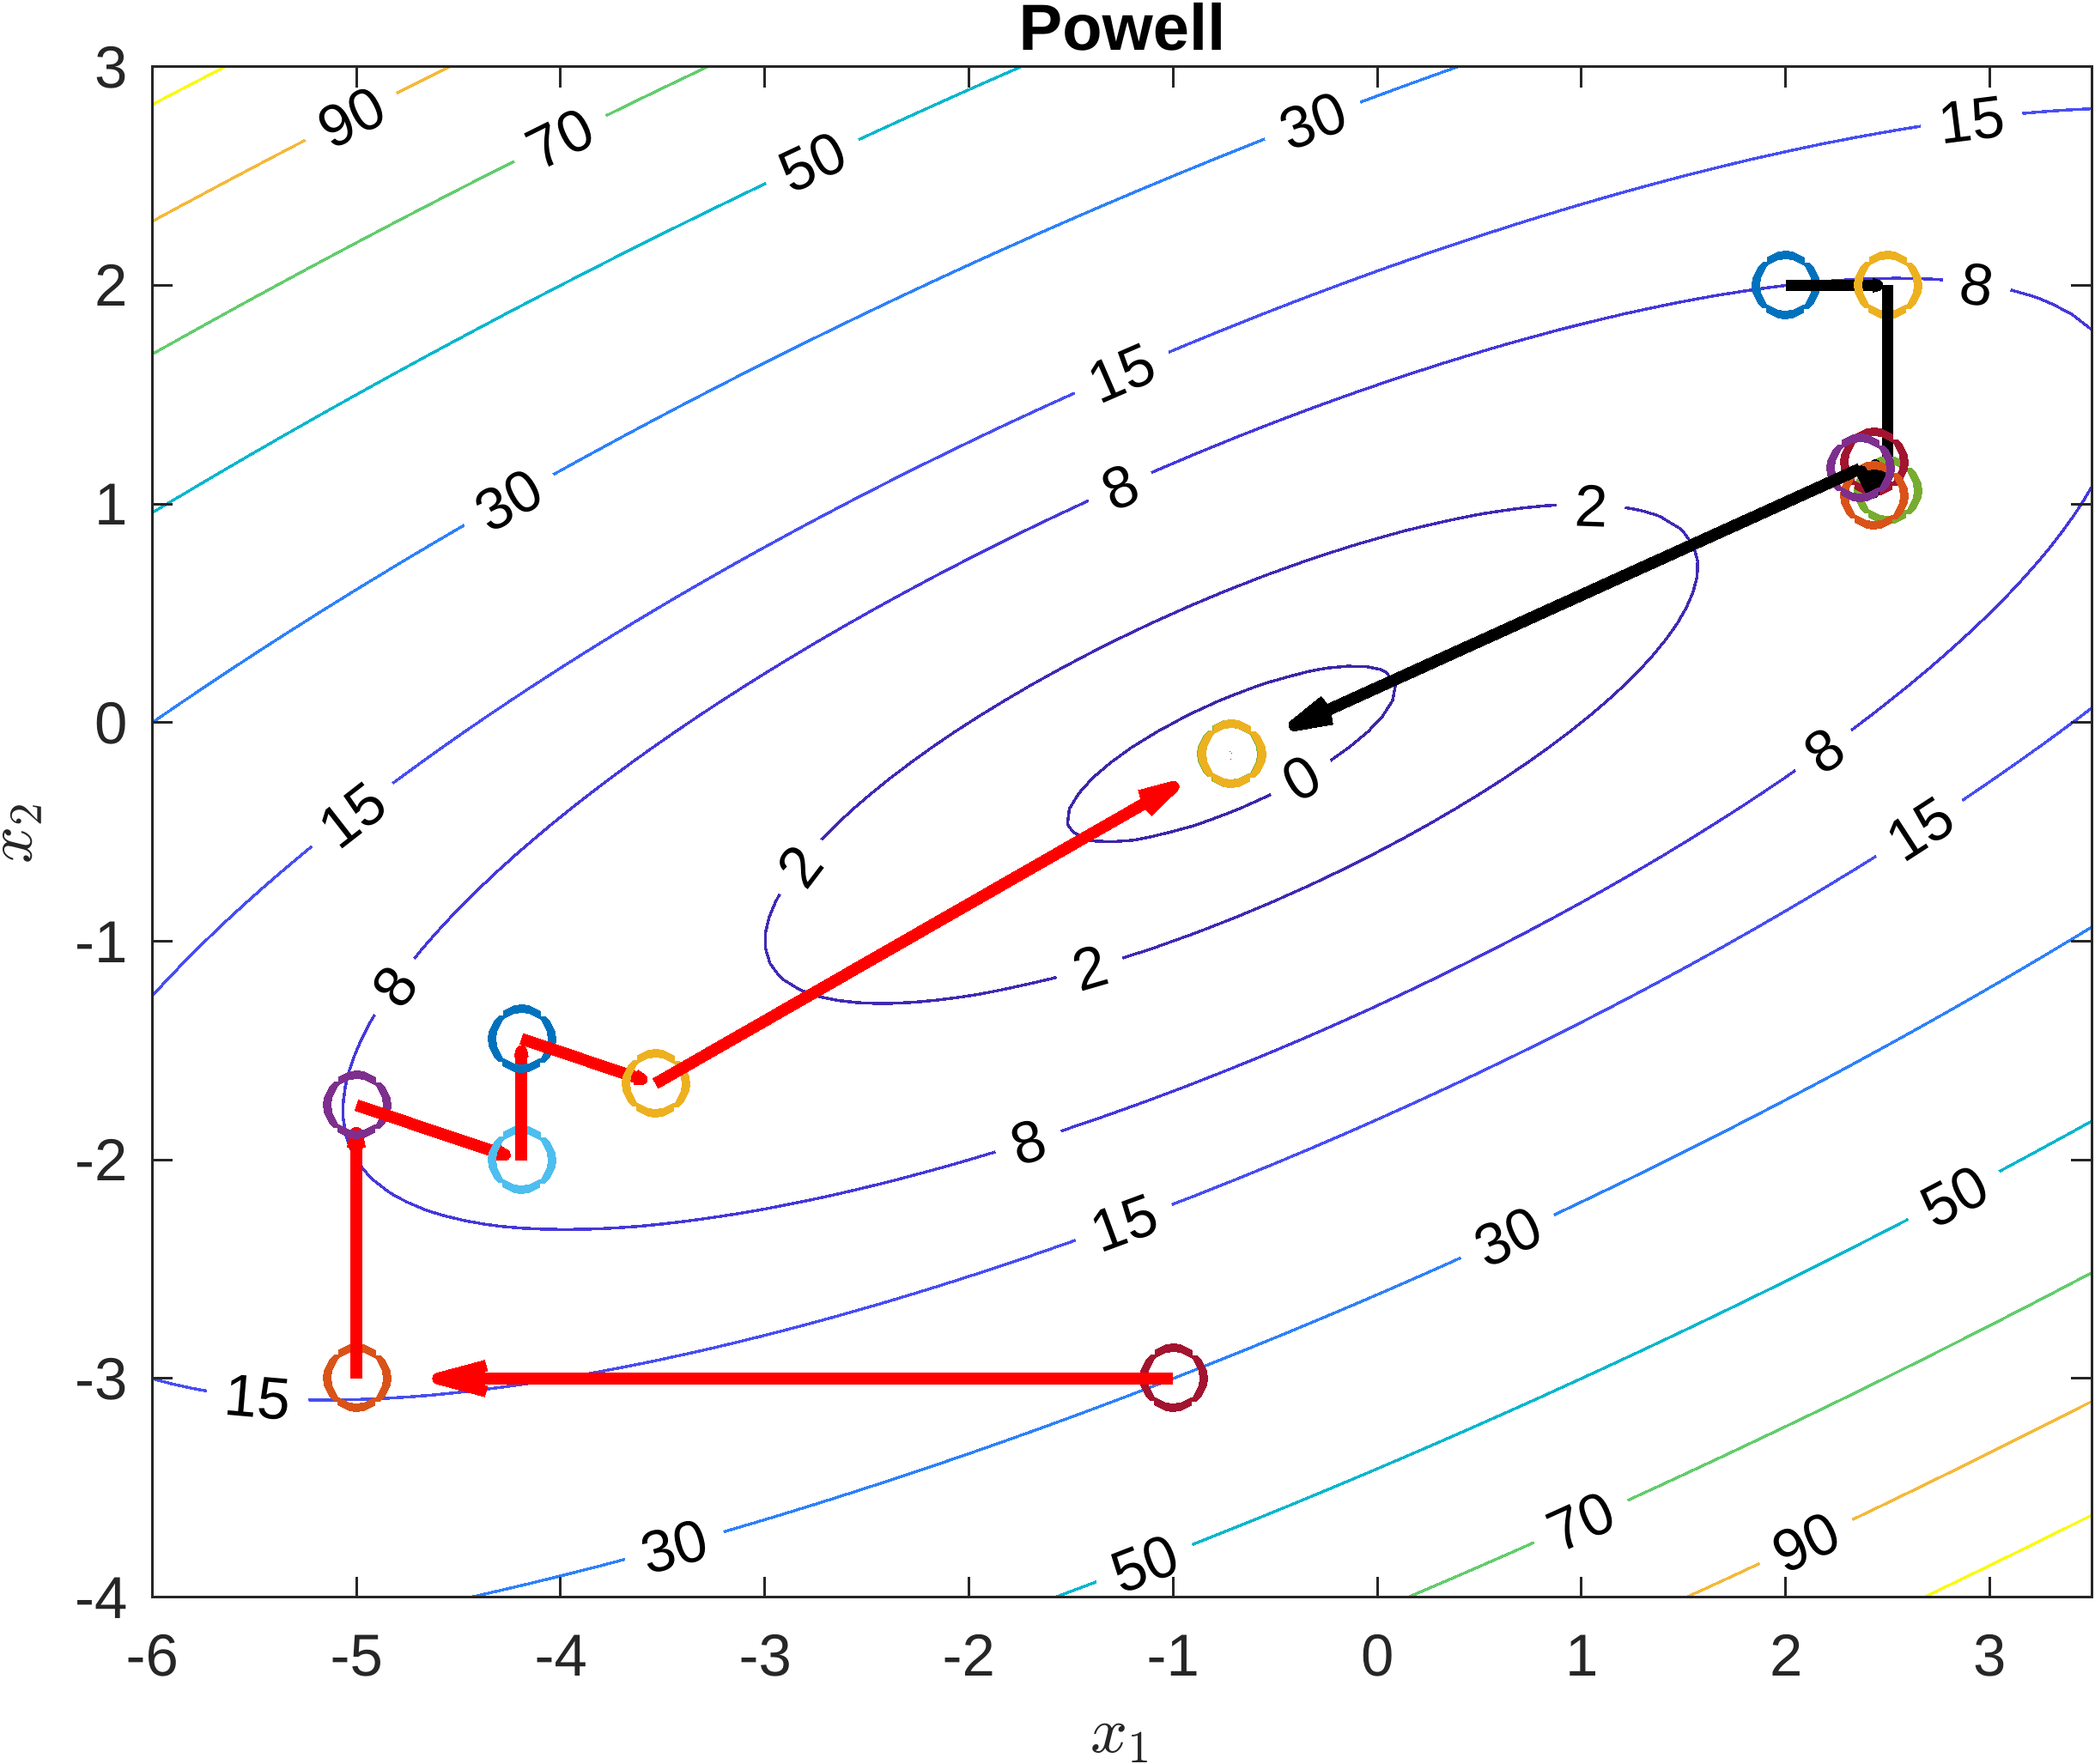
\includegraphics[width=\textwidth]{img01A_m02.png}
            \caption{Curvas de n\'ivel de $f_{1a}$ e pontos $x_{k}$}
            \label{fig:graf01A_m02}
      \end{subfigure}
      \begin{subfigure}{0.45\textwidth}
            \centering
            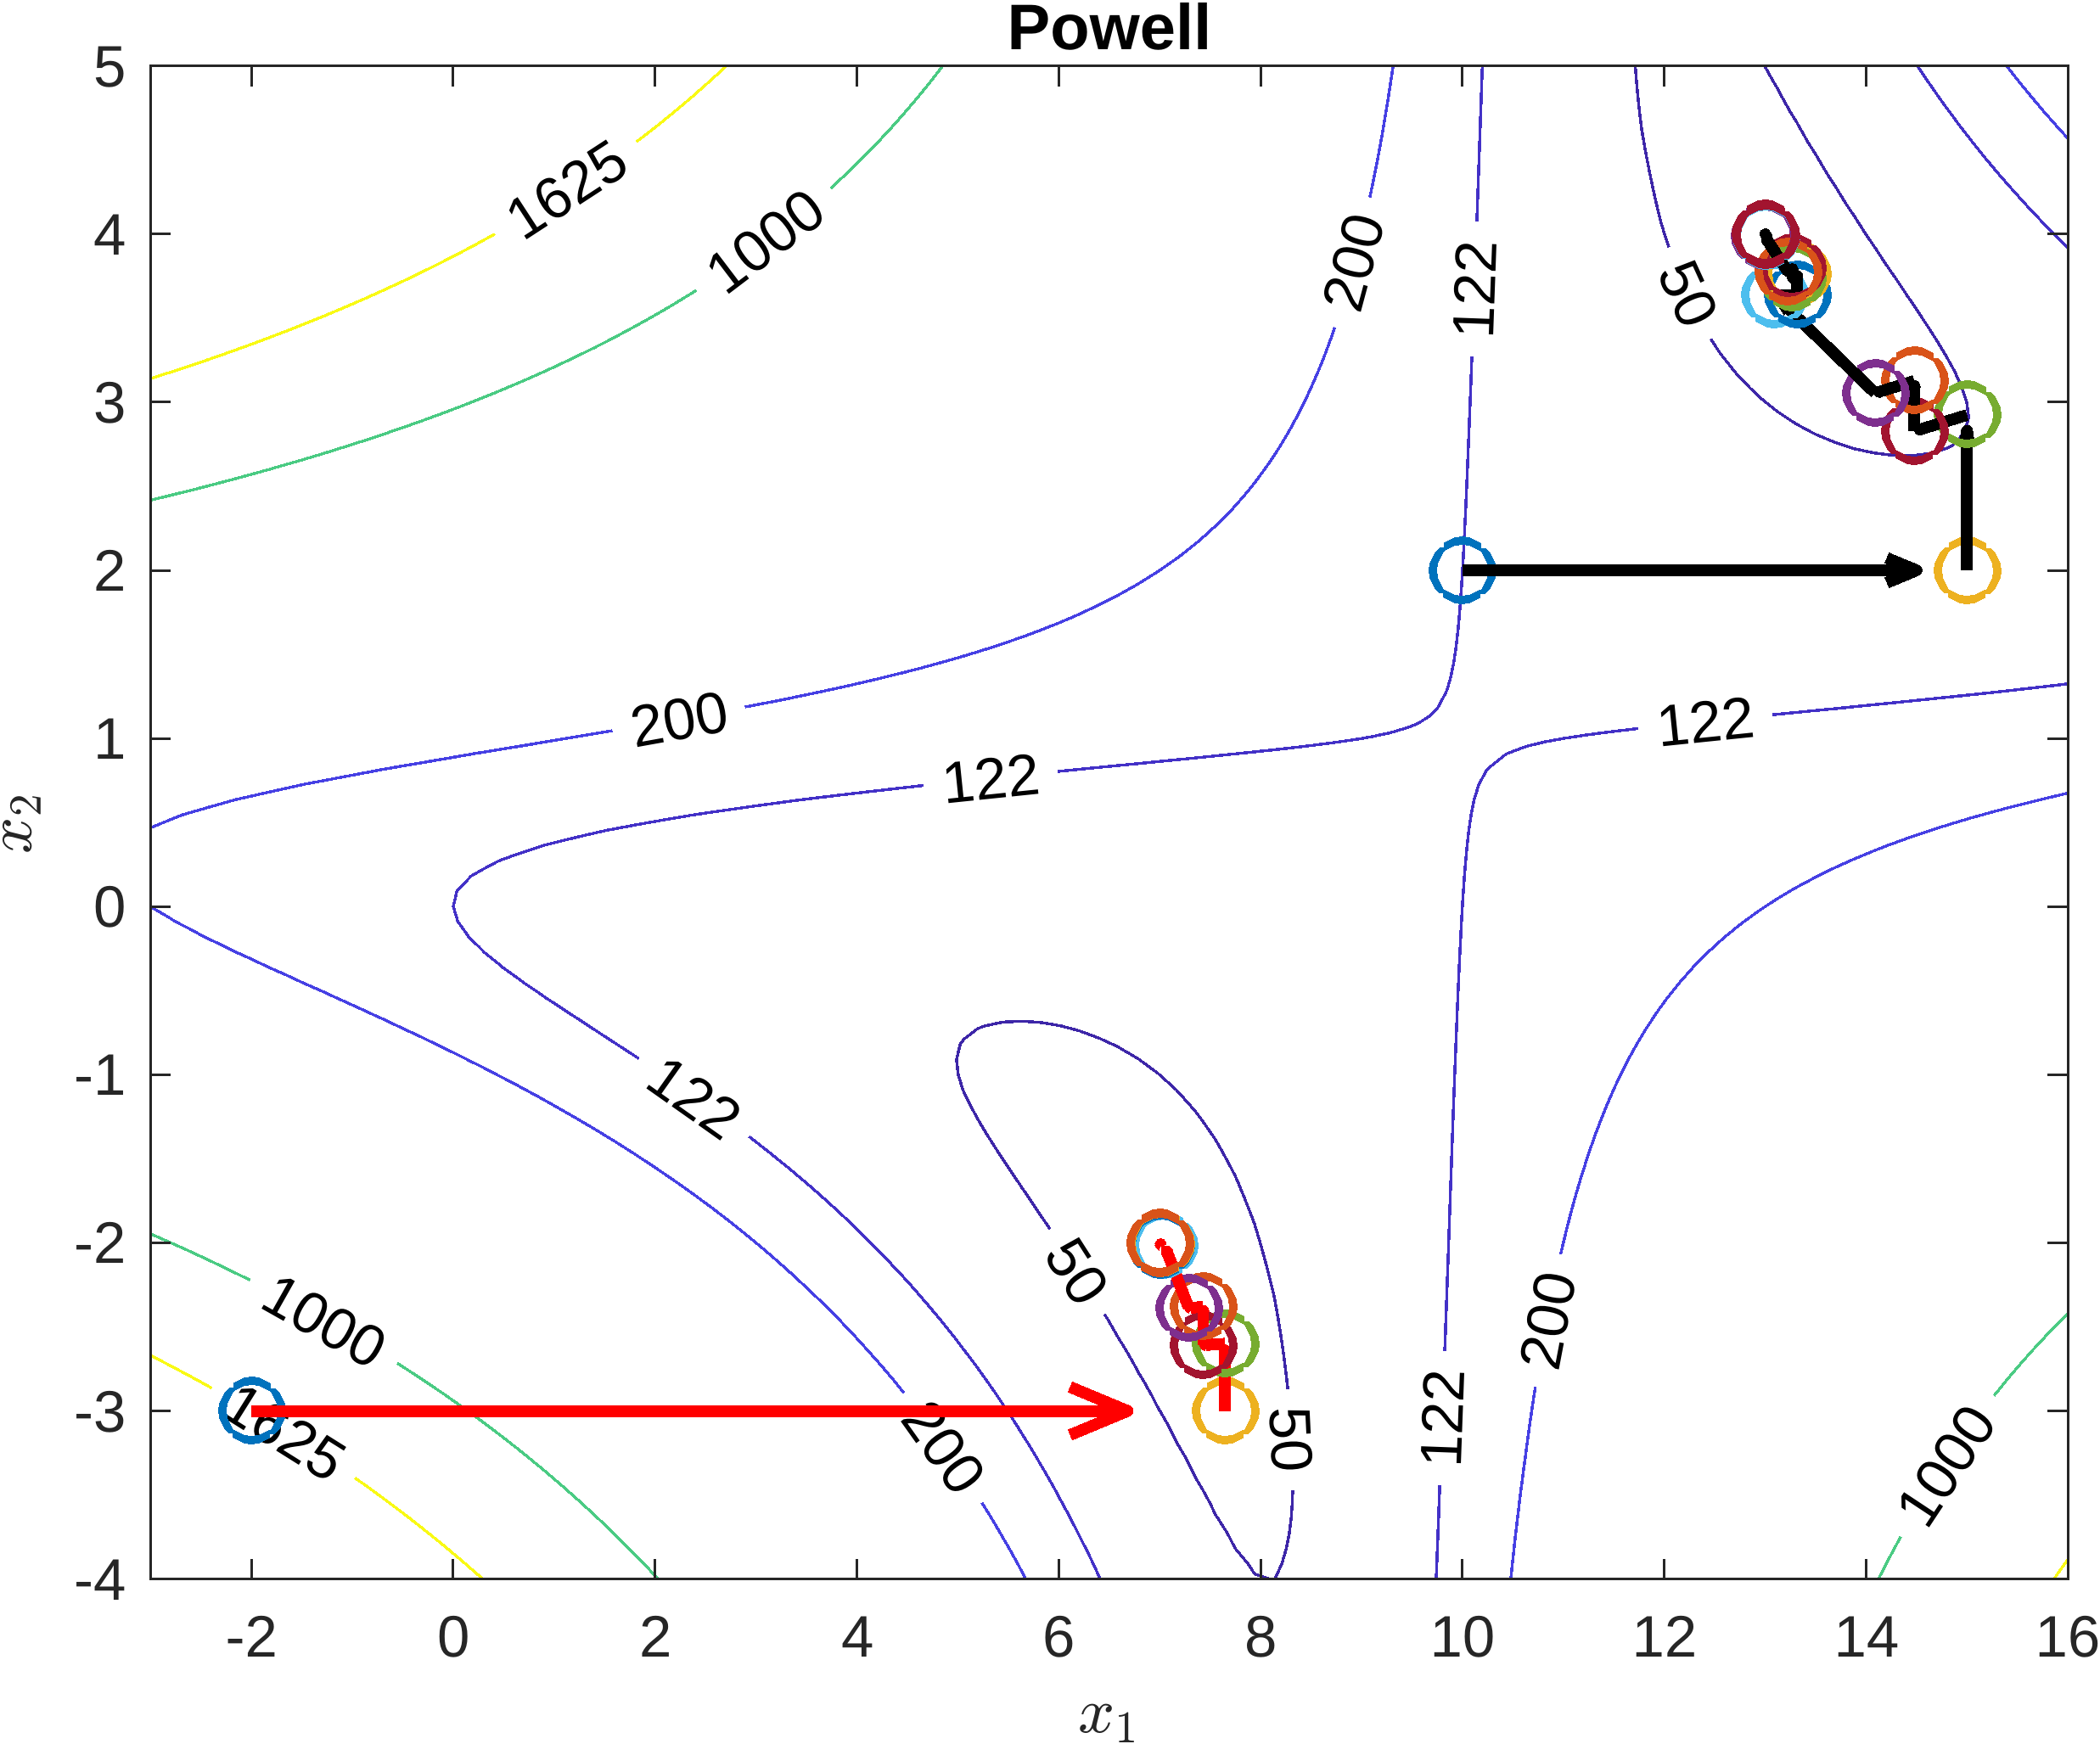
\includegraphics[width=\textwidth]{img01B_m02.png}
            \caption{Curvas de n\'ivel de $f_{1b}$ e pontos $x_{k}$}
            \label{fig:graf01B_m02}
      \end{subfigure}
      \caption{Resultados do m\'etodo de Powell, para as duas fun\c c\~oes e pontos iniciais}
      \label{fig:graf01_m02}
\end{figure}

\begin{figure}[H]
      \centering
      \begin{subfigure}{0.45\textwidth}
            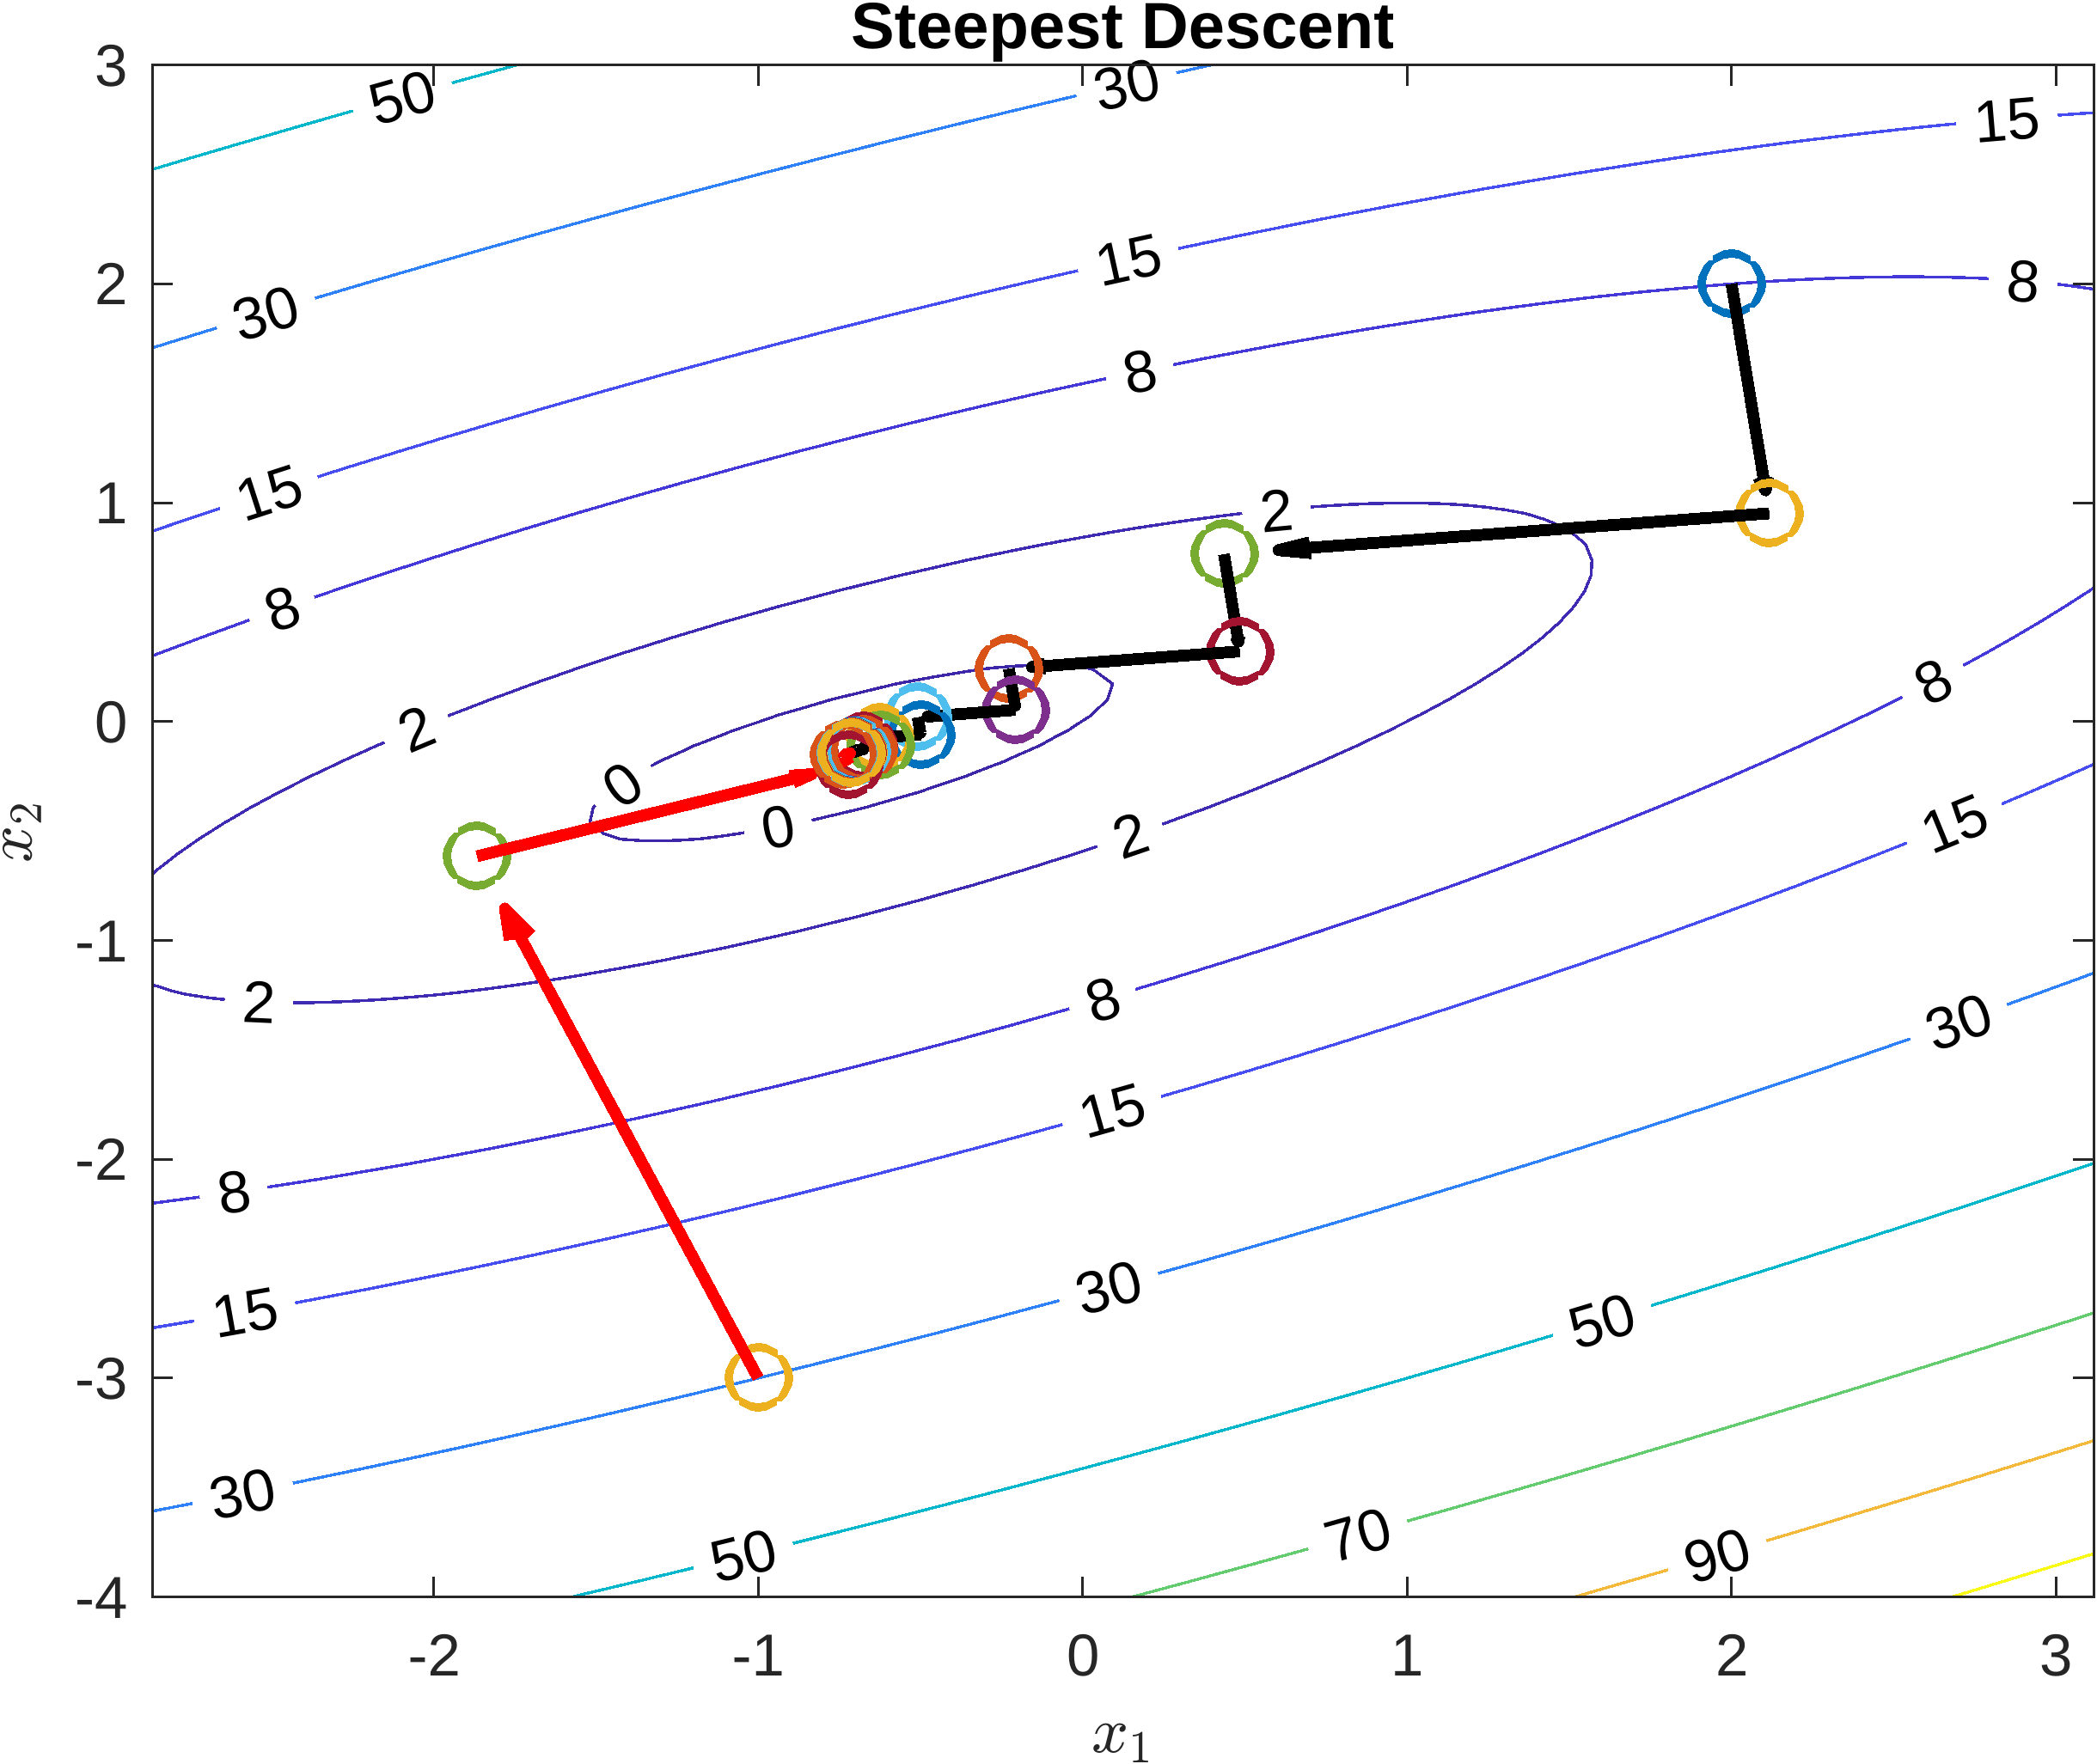
\includegraphics[width=\textwidth]{img01A_m03.png}
            \caption{Curvas de n\'ivel de $f_{1a}$ e pontos $x_{k}$}
            \label{fig:graf01A_m03}
      \end{subfigure}
      \begin{subfigure}{0.45\textwidth}
            \centering
            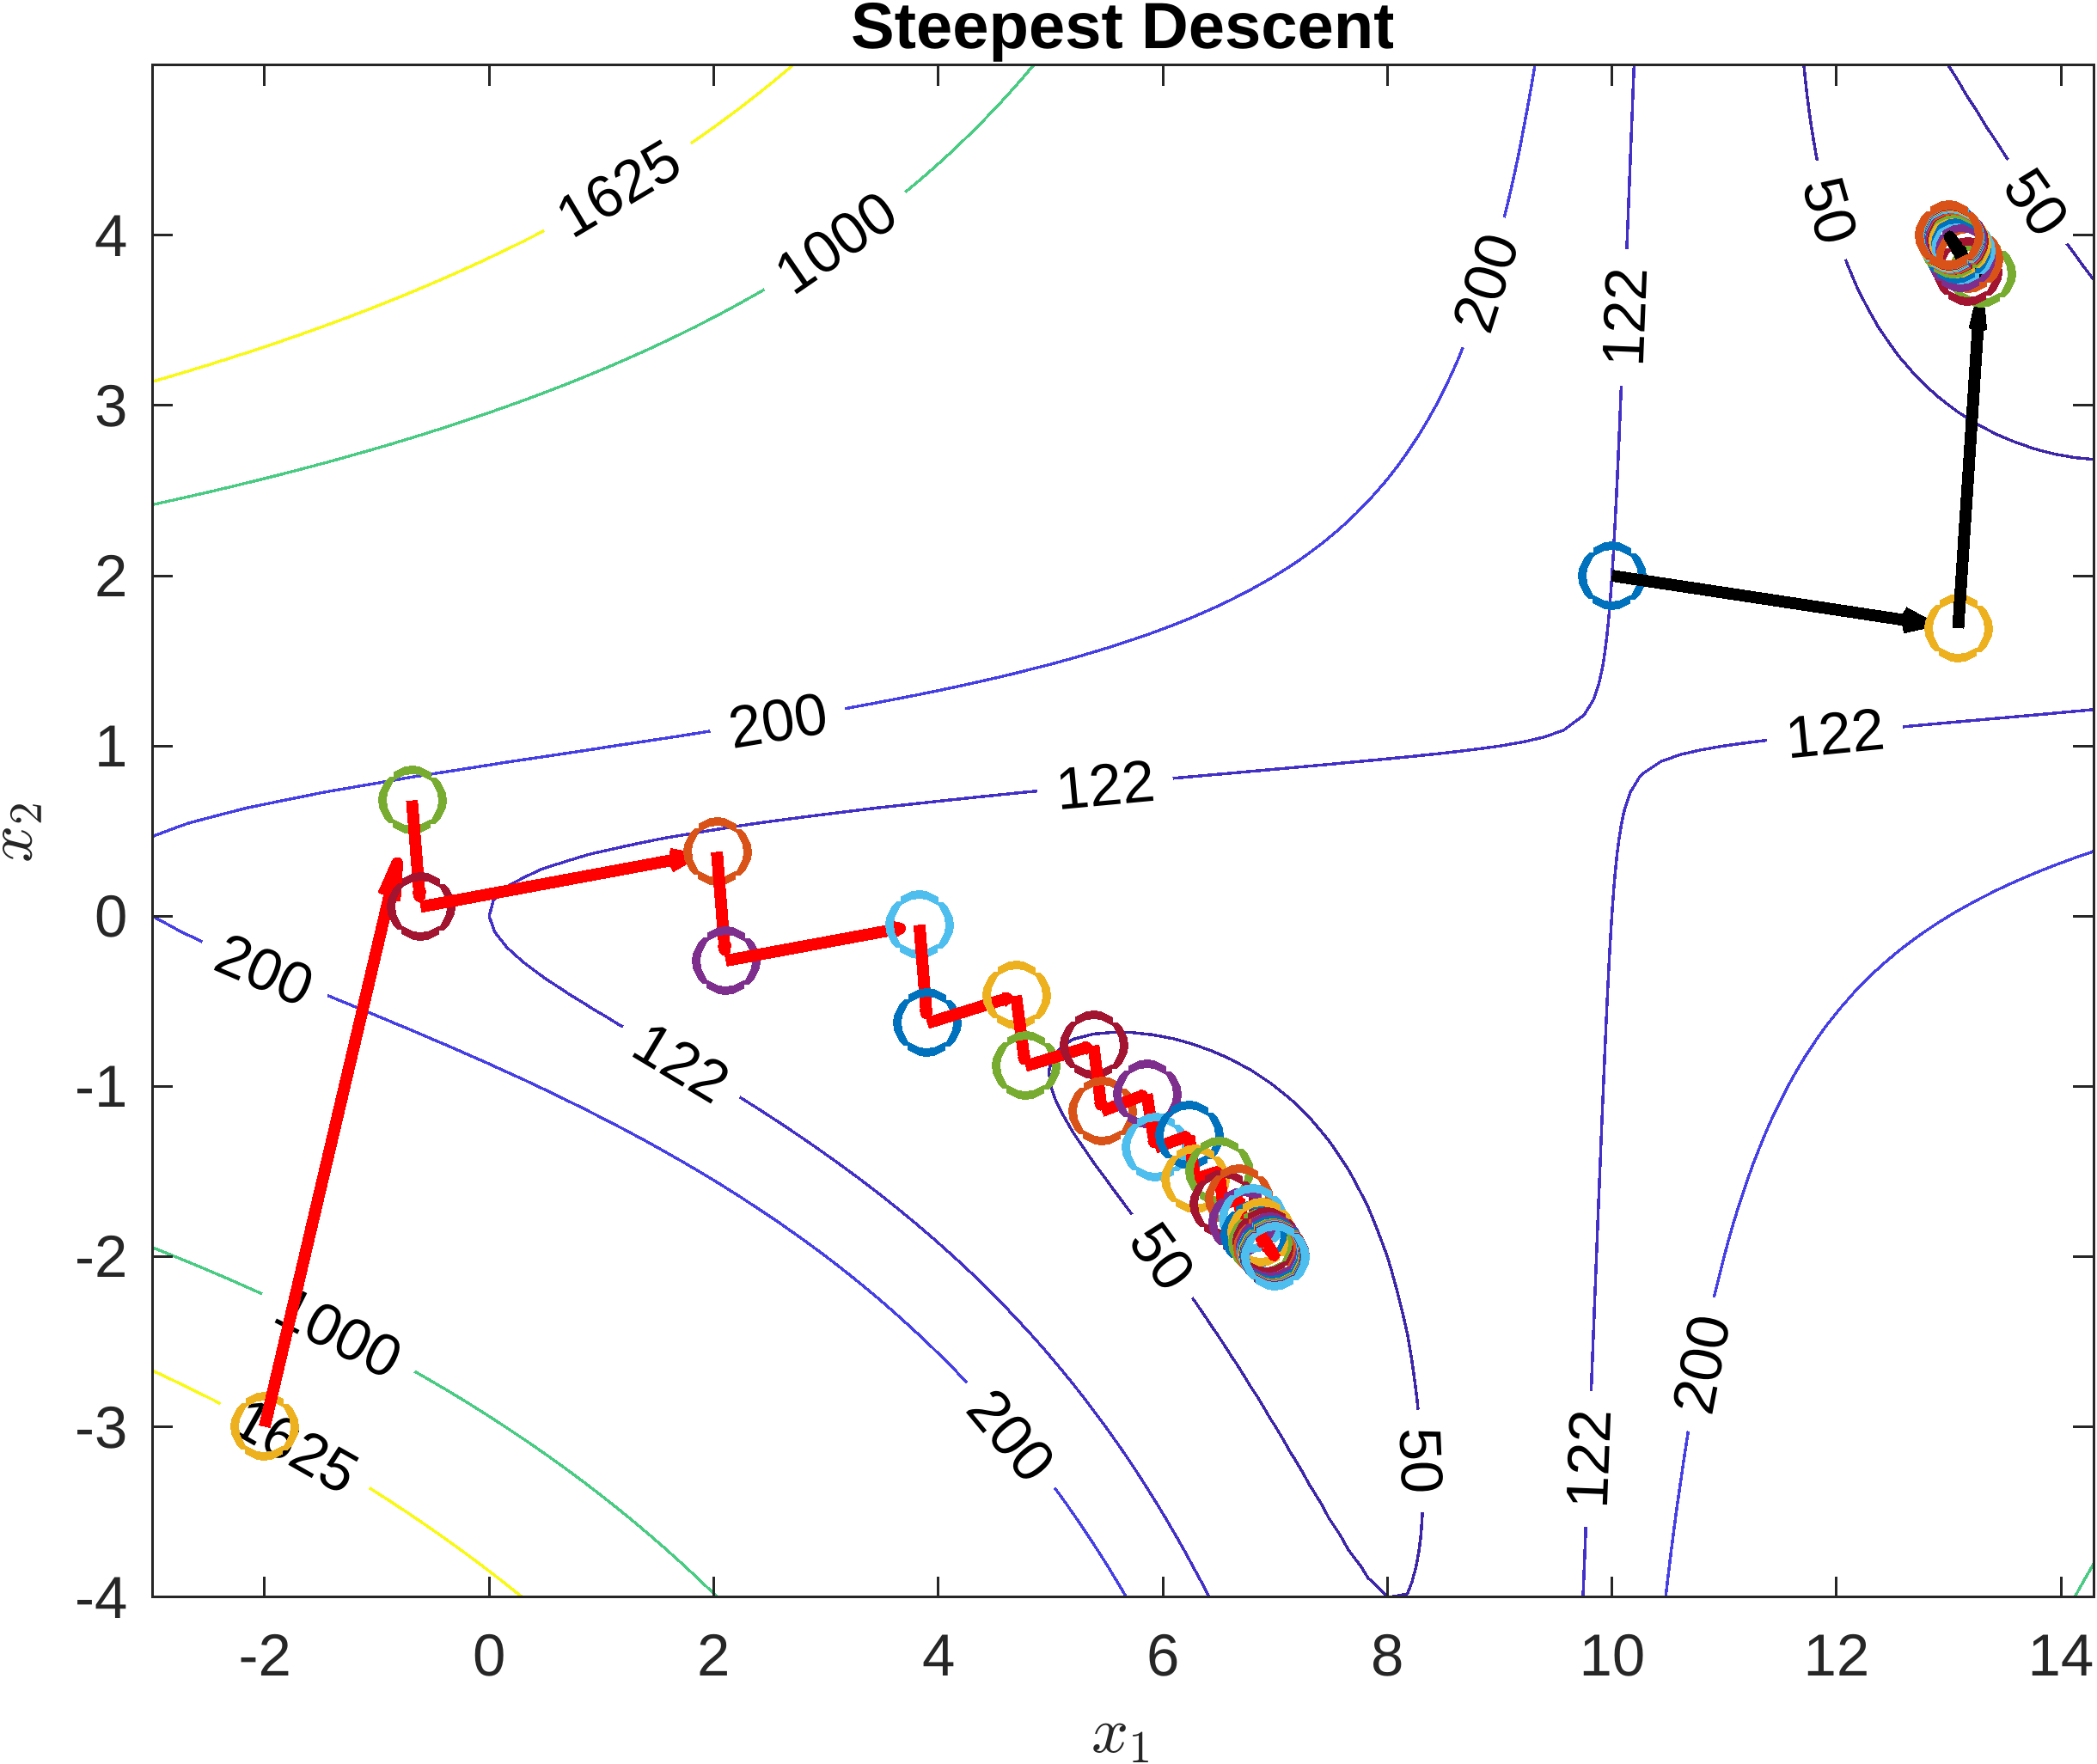
\includegraphics[width=\textwidth]{img01B_m03.png}
            \caption{Curvas de n\'ivel de $f_{1b}$ e pontos $x_{k}$}
            \label{fig:graf01B_m03}
      \end{subfigure}
      \caption{Resultados do m\'etodo Steepest Descent, para as duas fun\c c\~oes e pontos iniciais}
      \label{fig:graf01_m03}
\end{figure}

\begin{figure}[H]
      \centering
      \begin{subfigure}{0.45\textwidth}
            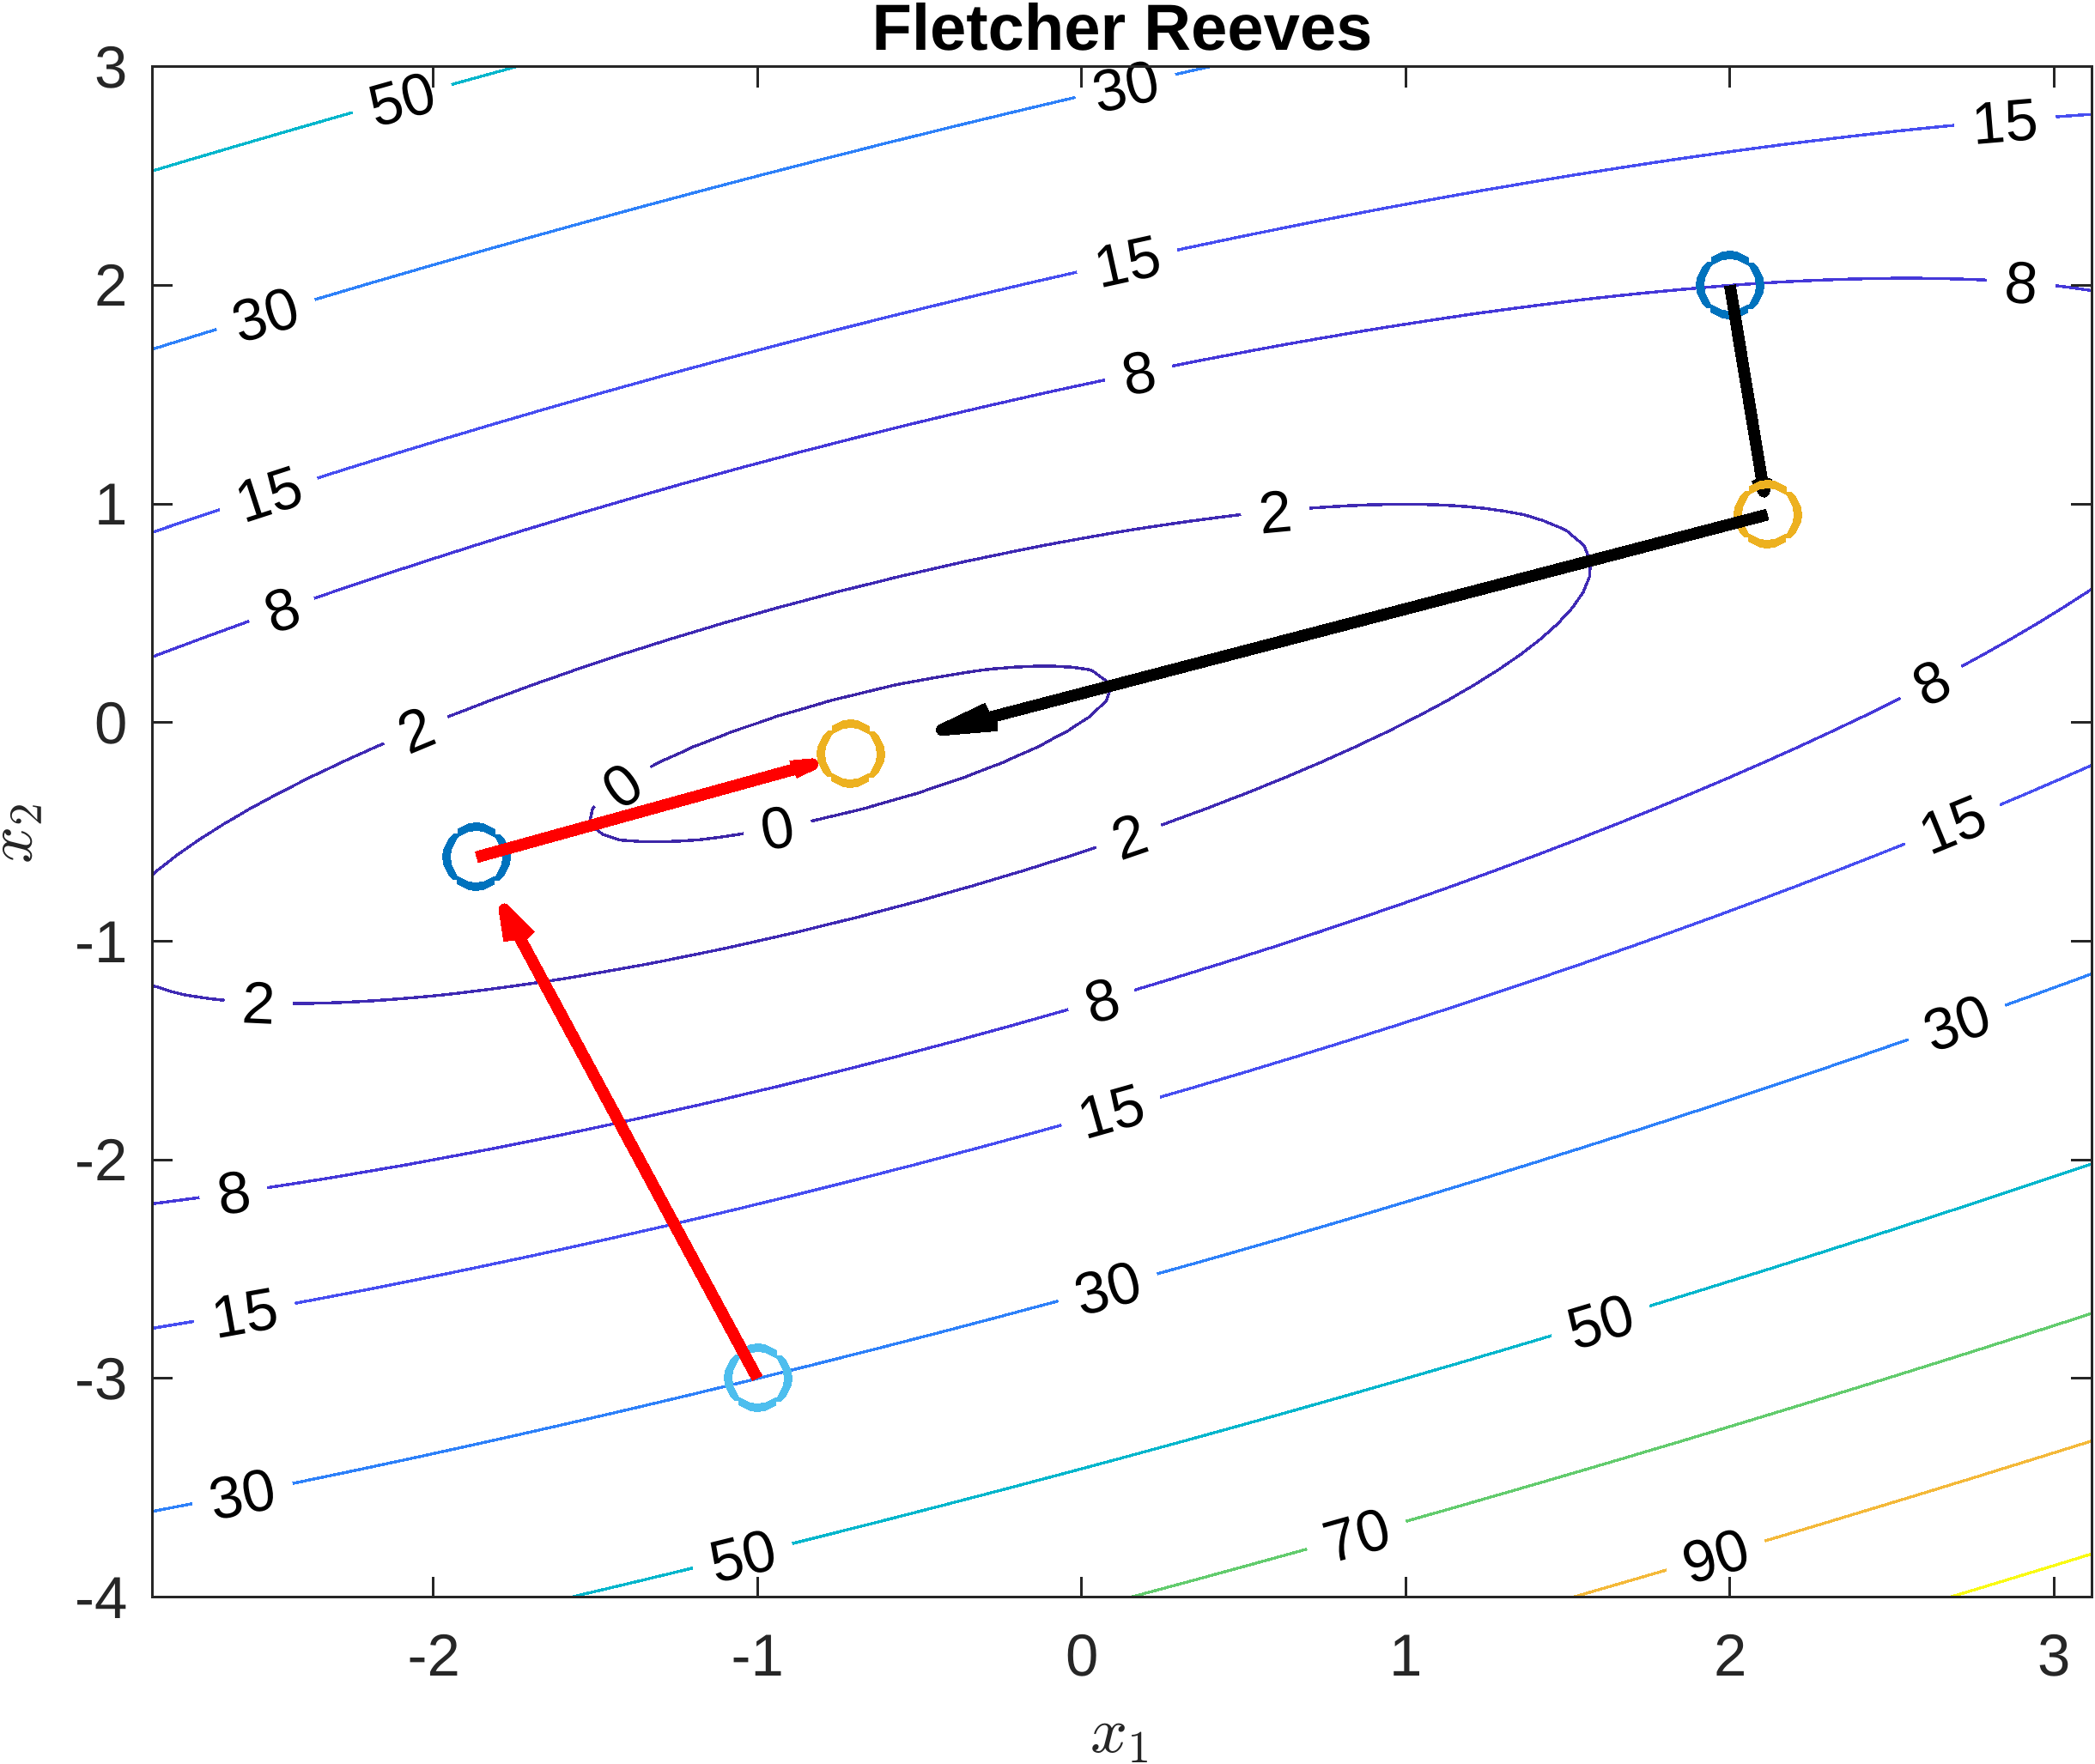
\includegraphics[width=\textwidth]{img01A_m04.png}
            \caption{Curvas de n\'ivel de $f_{1a}$ e pontos $x_{k}$}
            \label{fig:graf01A_m04}
      \end{subfigure}
      \begin{subfigure}{0.45\textwidth}
            \centering
            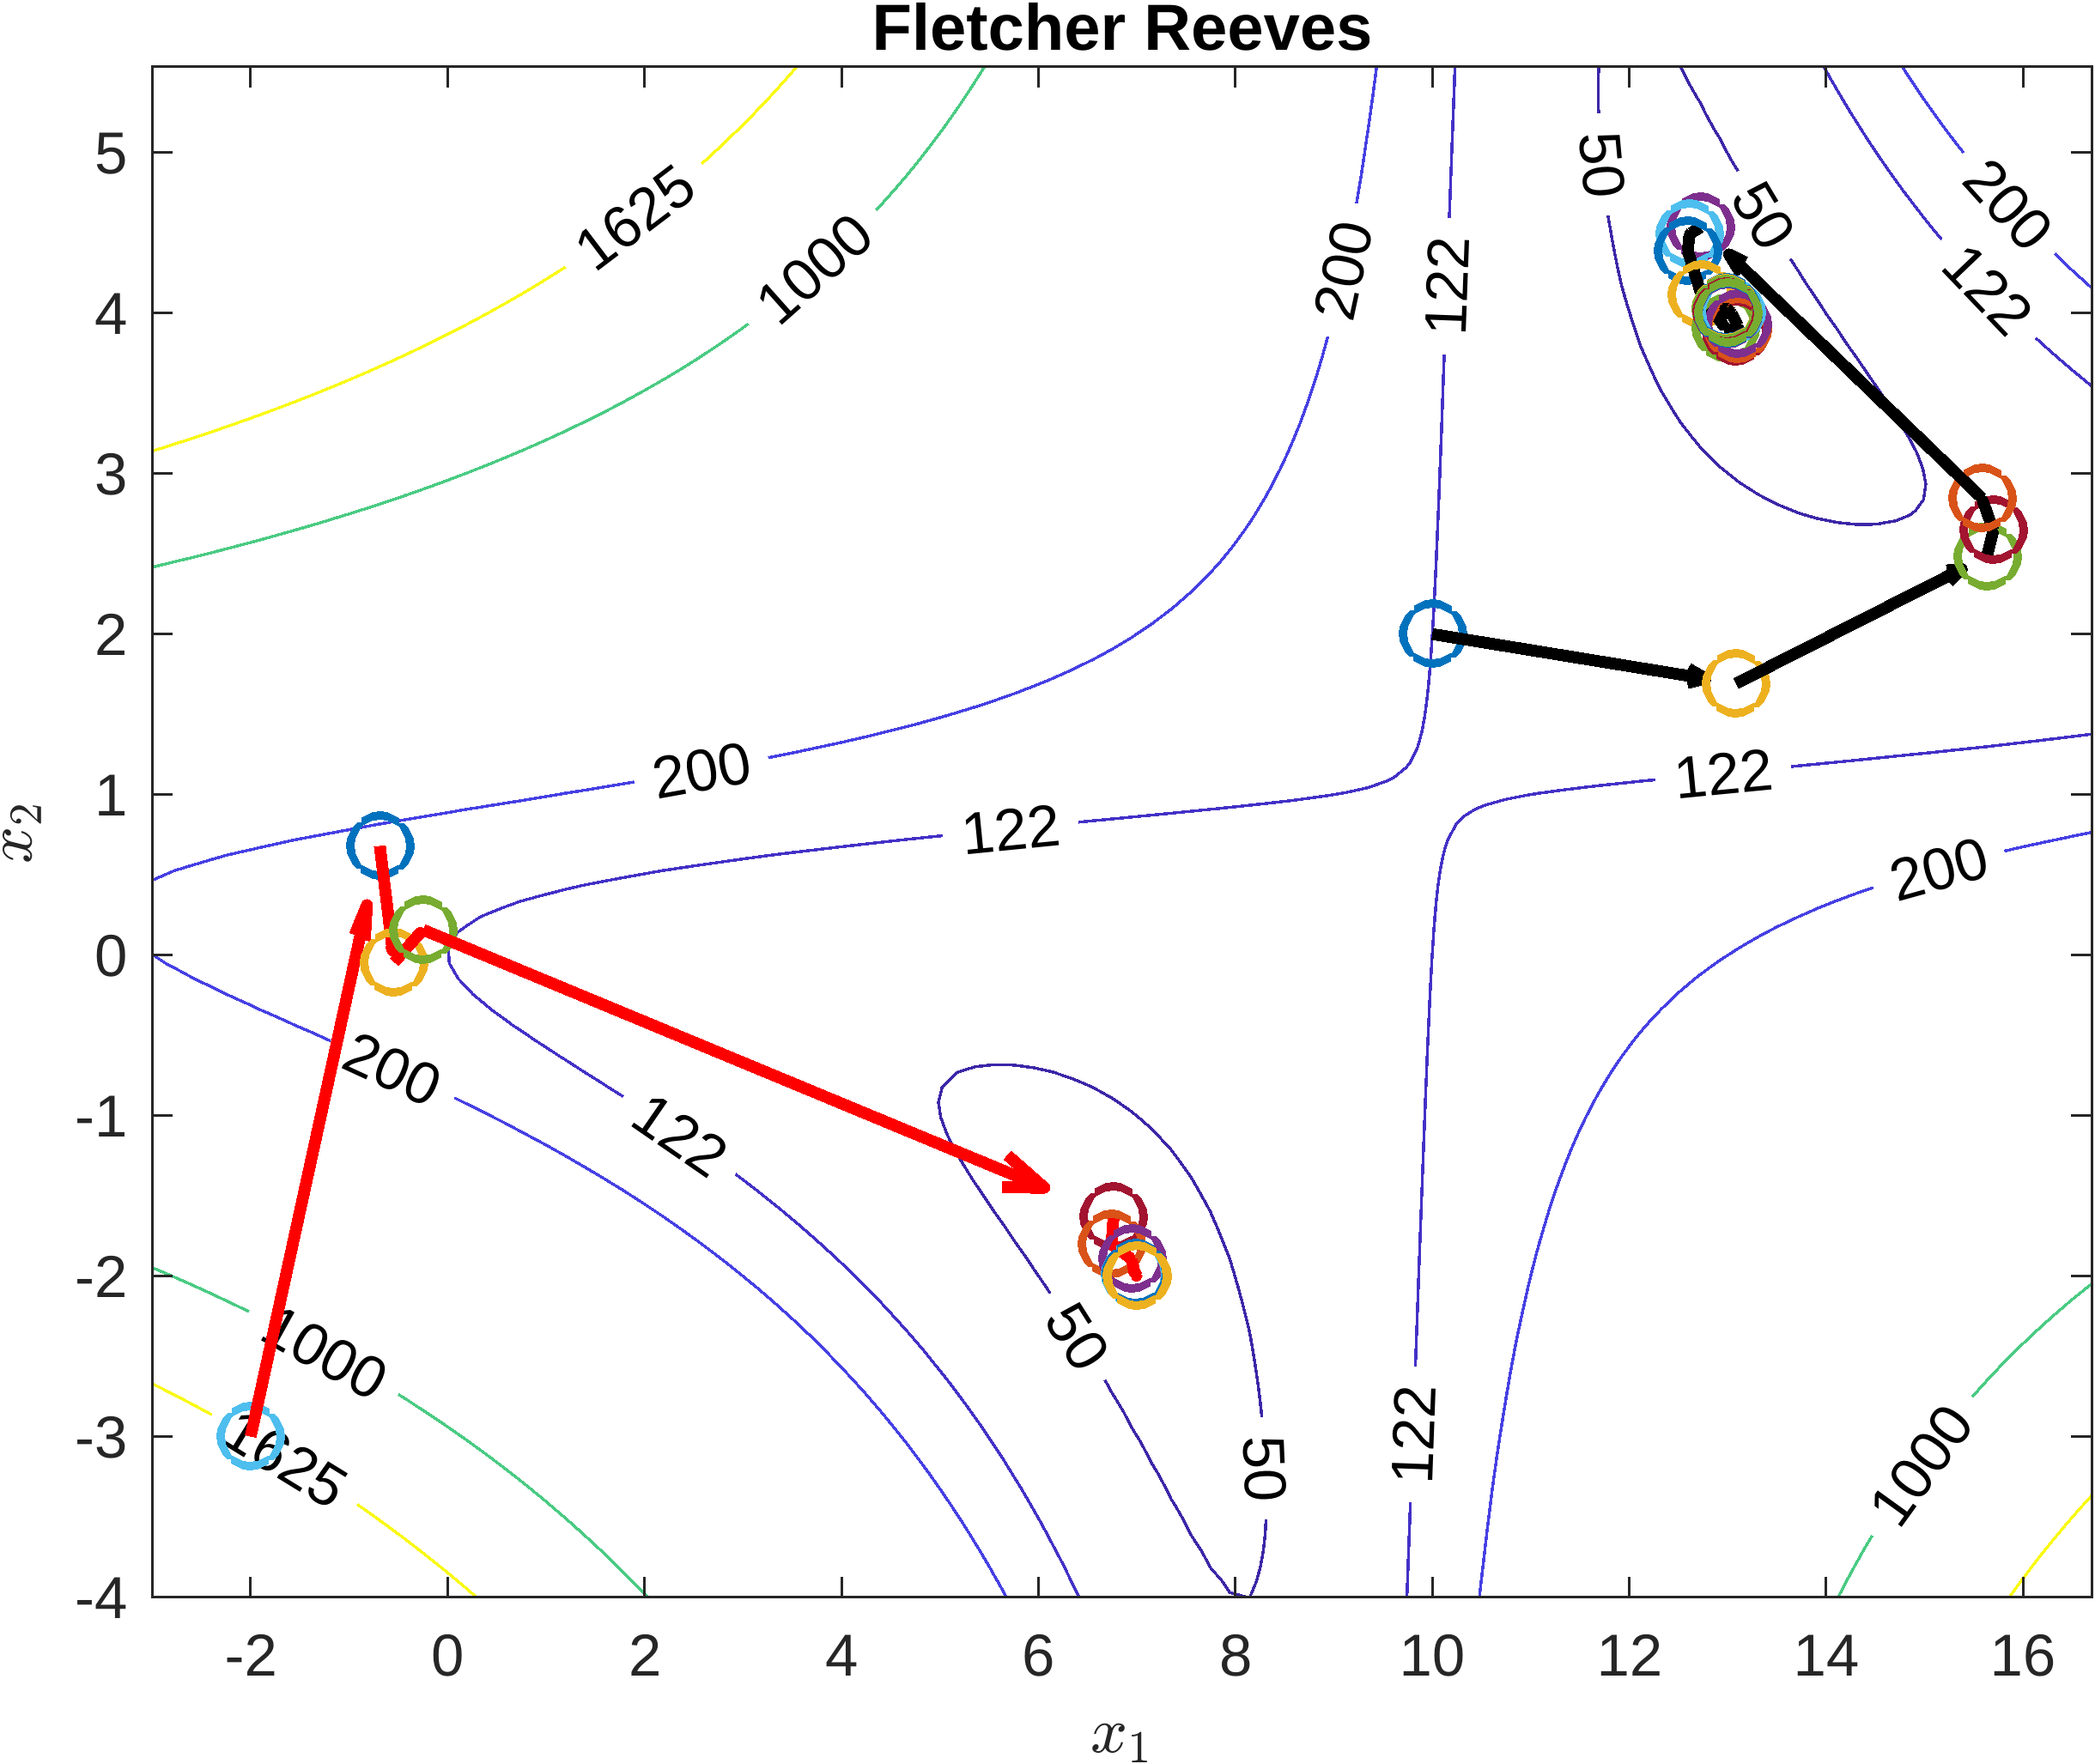
\includegraphics[width=\textwidth]{img01B_m04.png}
            \caption{Curvas de n\'ivel de $f_{1b}$ e pontos $x_{k}$}
            \label{fig:graf01B_m04}
      \end{subfigure}
      \caption{Resultados do m\'etodo Fletcher-Reeves, para as duas fun\c c\~oes e pontos iniciais}
      \label{fig:graf01_m04}
\end{figure}

\begin{figure}[H]
      \centering
      \begin{subfigure}{0.45\textwidth}
            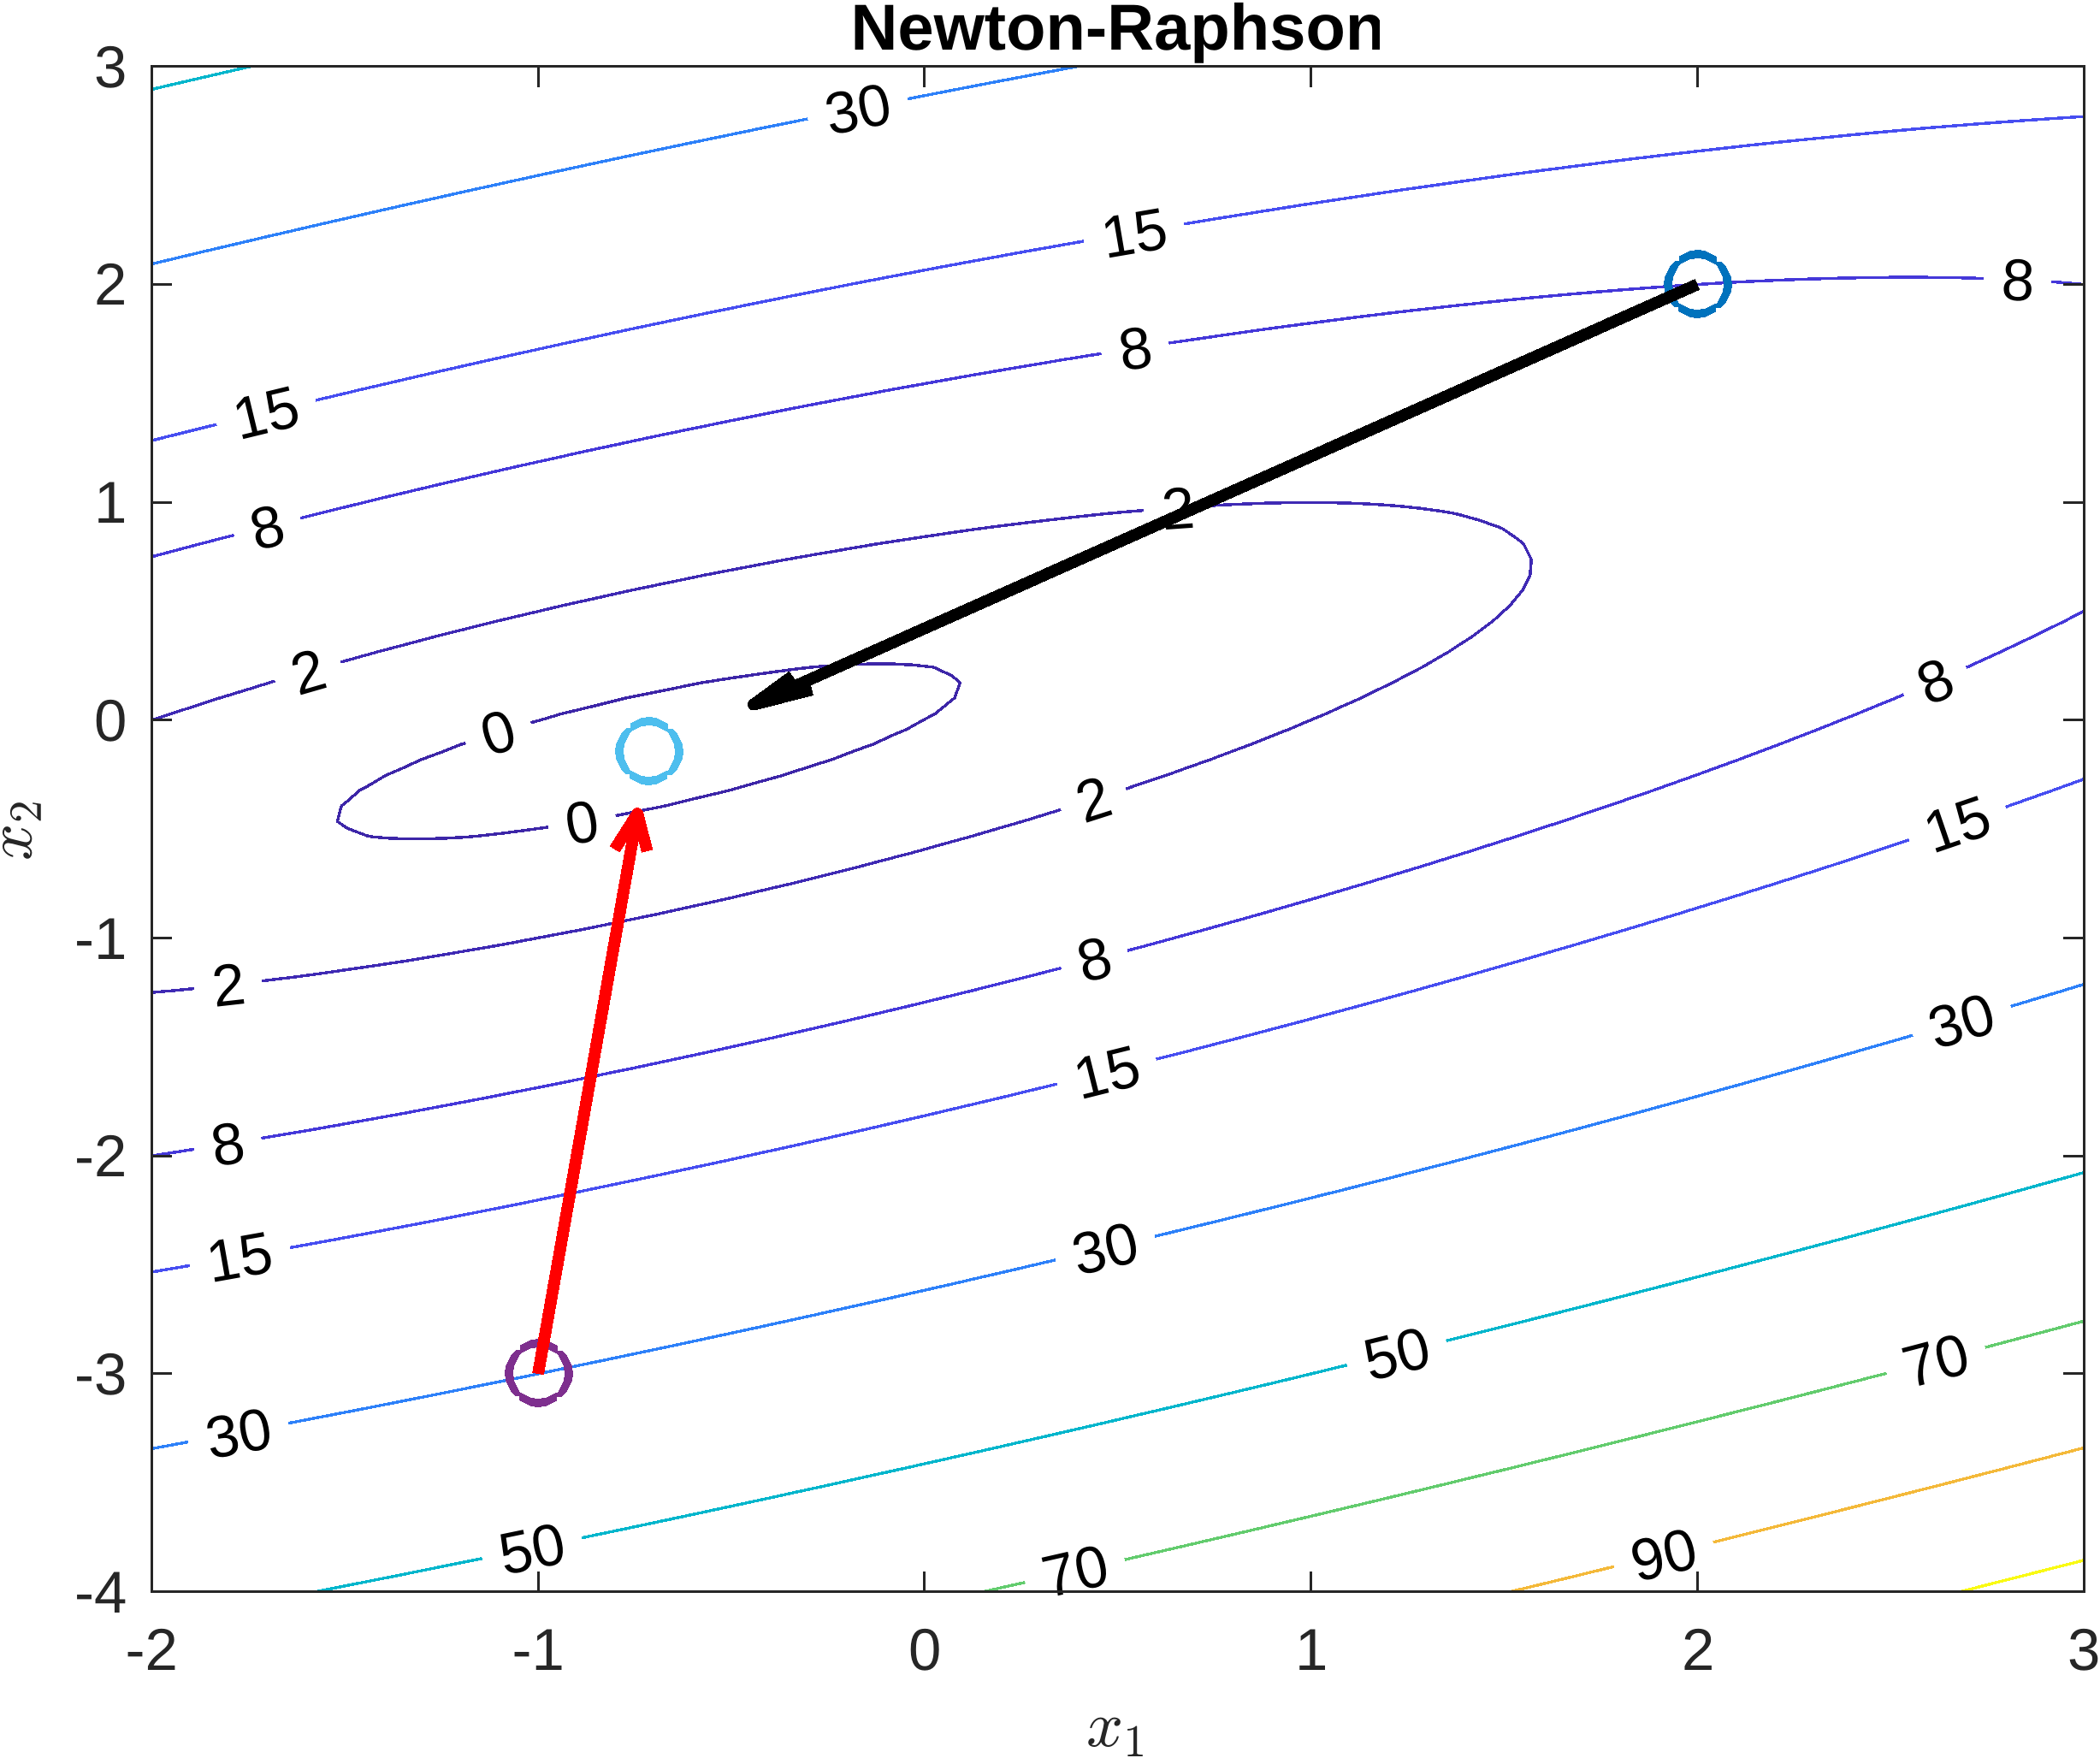
\includegraphics[width=\textwidth]{img01A_m05.png}
            \caption{Curvas de n\'ivel de $f_{1a}$ e pontos $x_{k}$}
            \label{fig:graf01A_m05}
      \end{subfigure}
      \begin{subfigure}{0.45\textwidth}
            \centering
            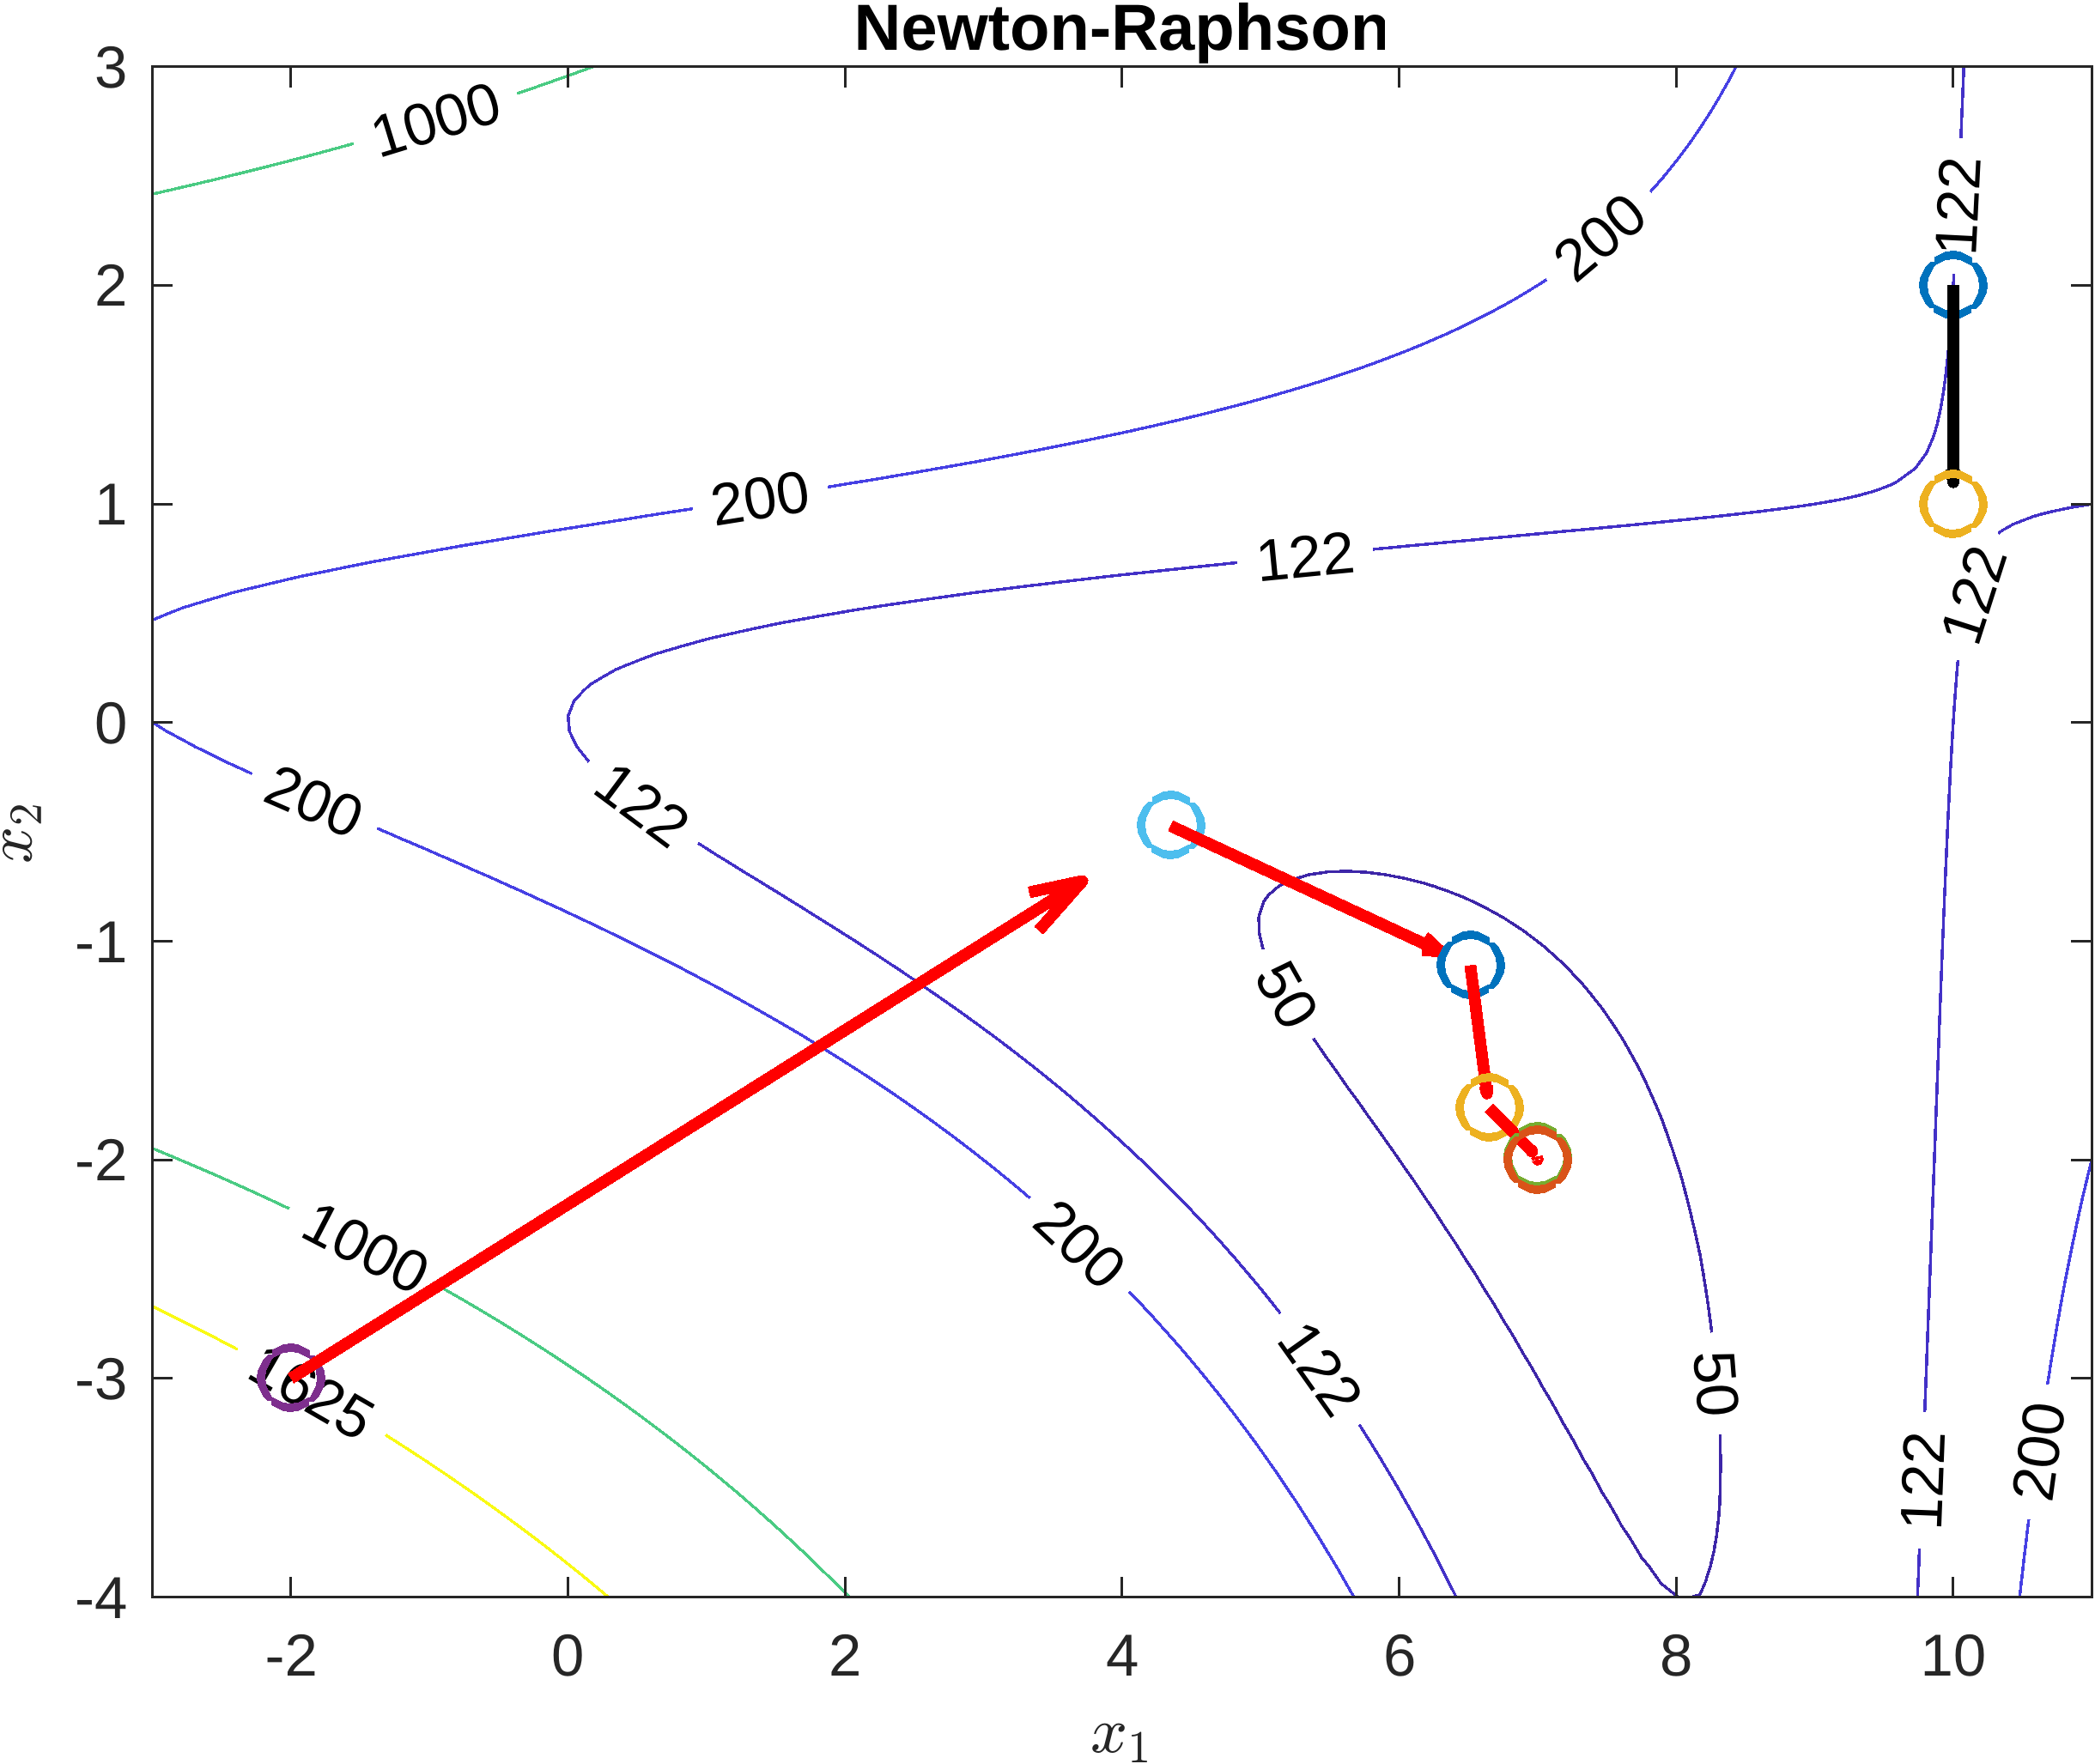
\includegraphics[width=\textwidth]{img01B_m05.png}
            \caption{Curvas de n\'ivel de $f_{1b}$ e pontos $x_{k}$}
            \label{fig:graf01B_m05}
      \end{subfigure}
      \caption{Resultados do m\'etodo Newton-Raphson, para as duas fun\c c\~oes e pontos iniciais}
      \label{fig:graf01_m05}
\end{figure}

\begin{figure}[H]
      \centering
      \begin{subfigure}{0.45\textwidth}
            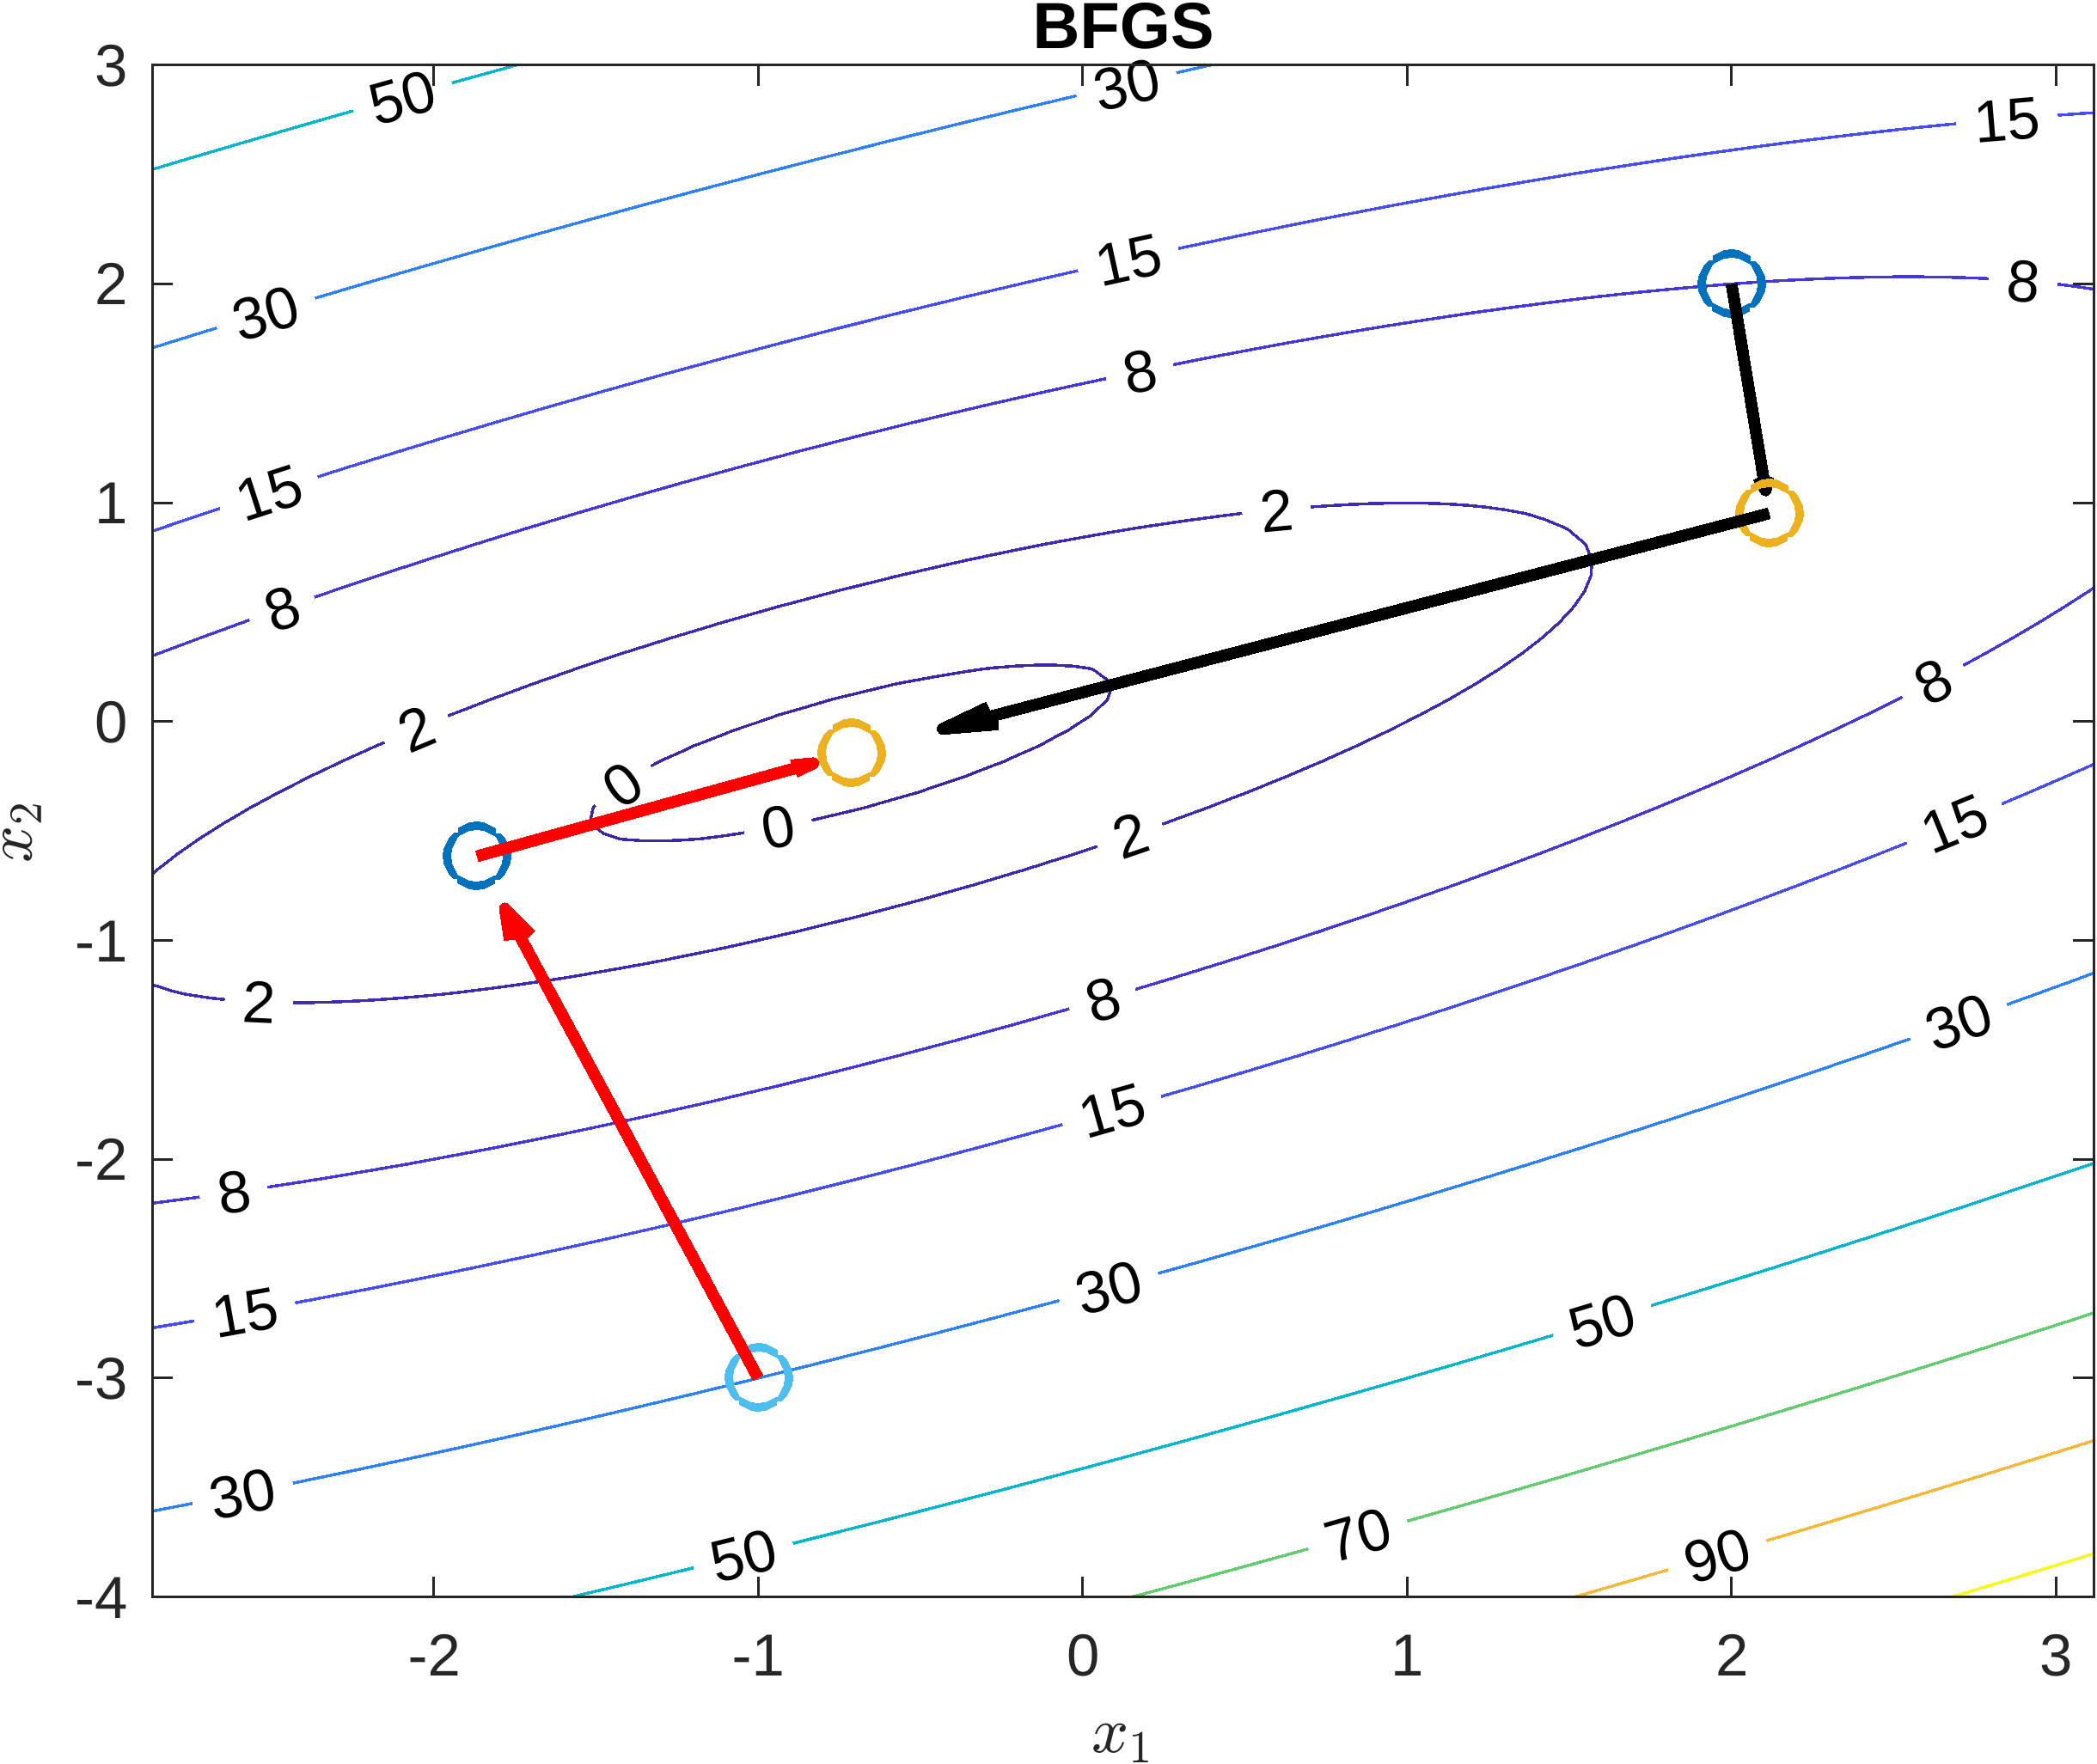
\includegraphics[width=\textwidth]{img01A_m06.png}
            \caption{Curvas de n\'ivel de $f_{1a}$ e pontos $x_{k}$}
            \label{fig:graf01A_m06}
      \end{subfigure}
      \begin{subfigure}{0.45\textwidth}
            \centering
            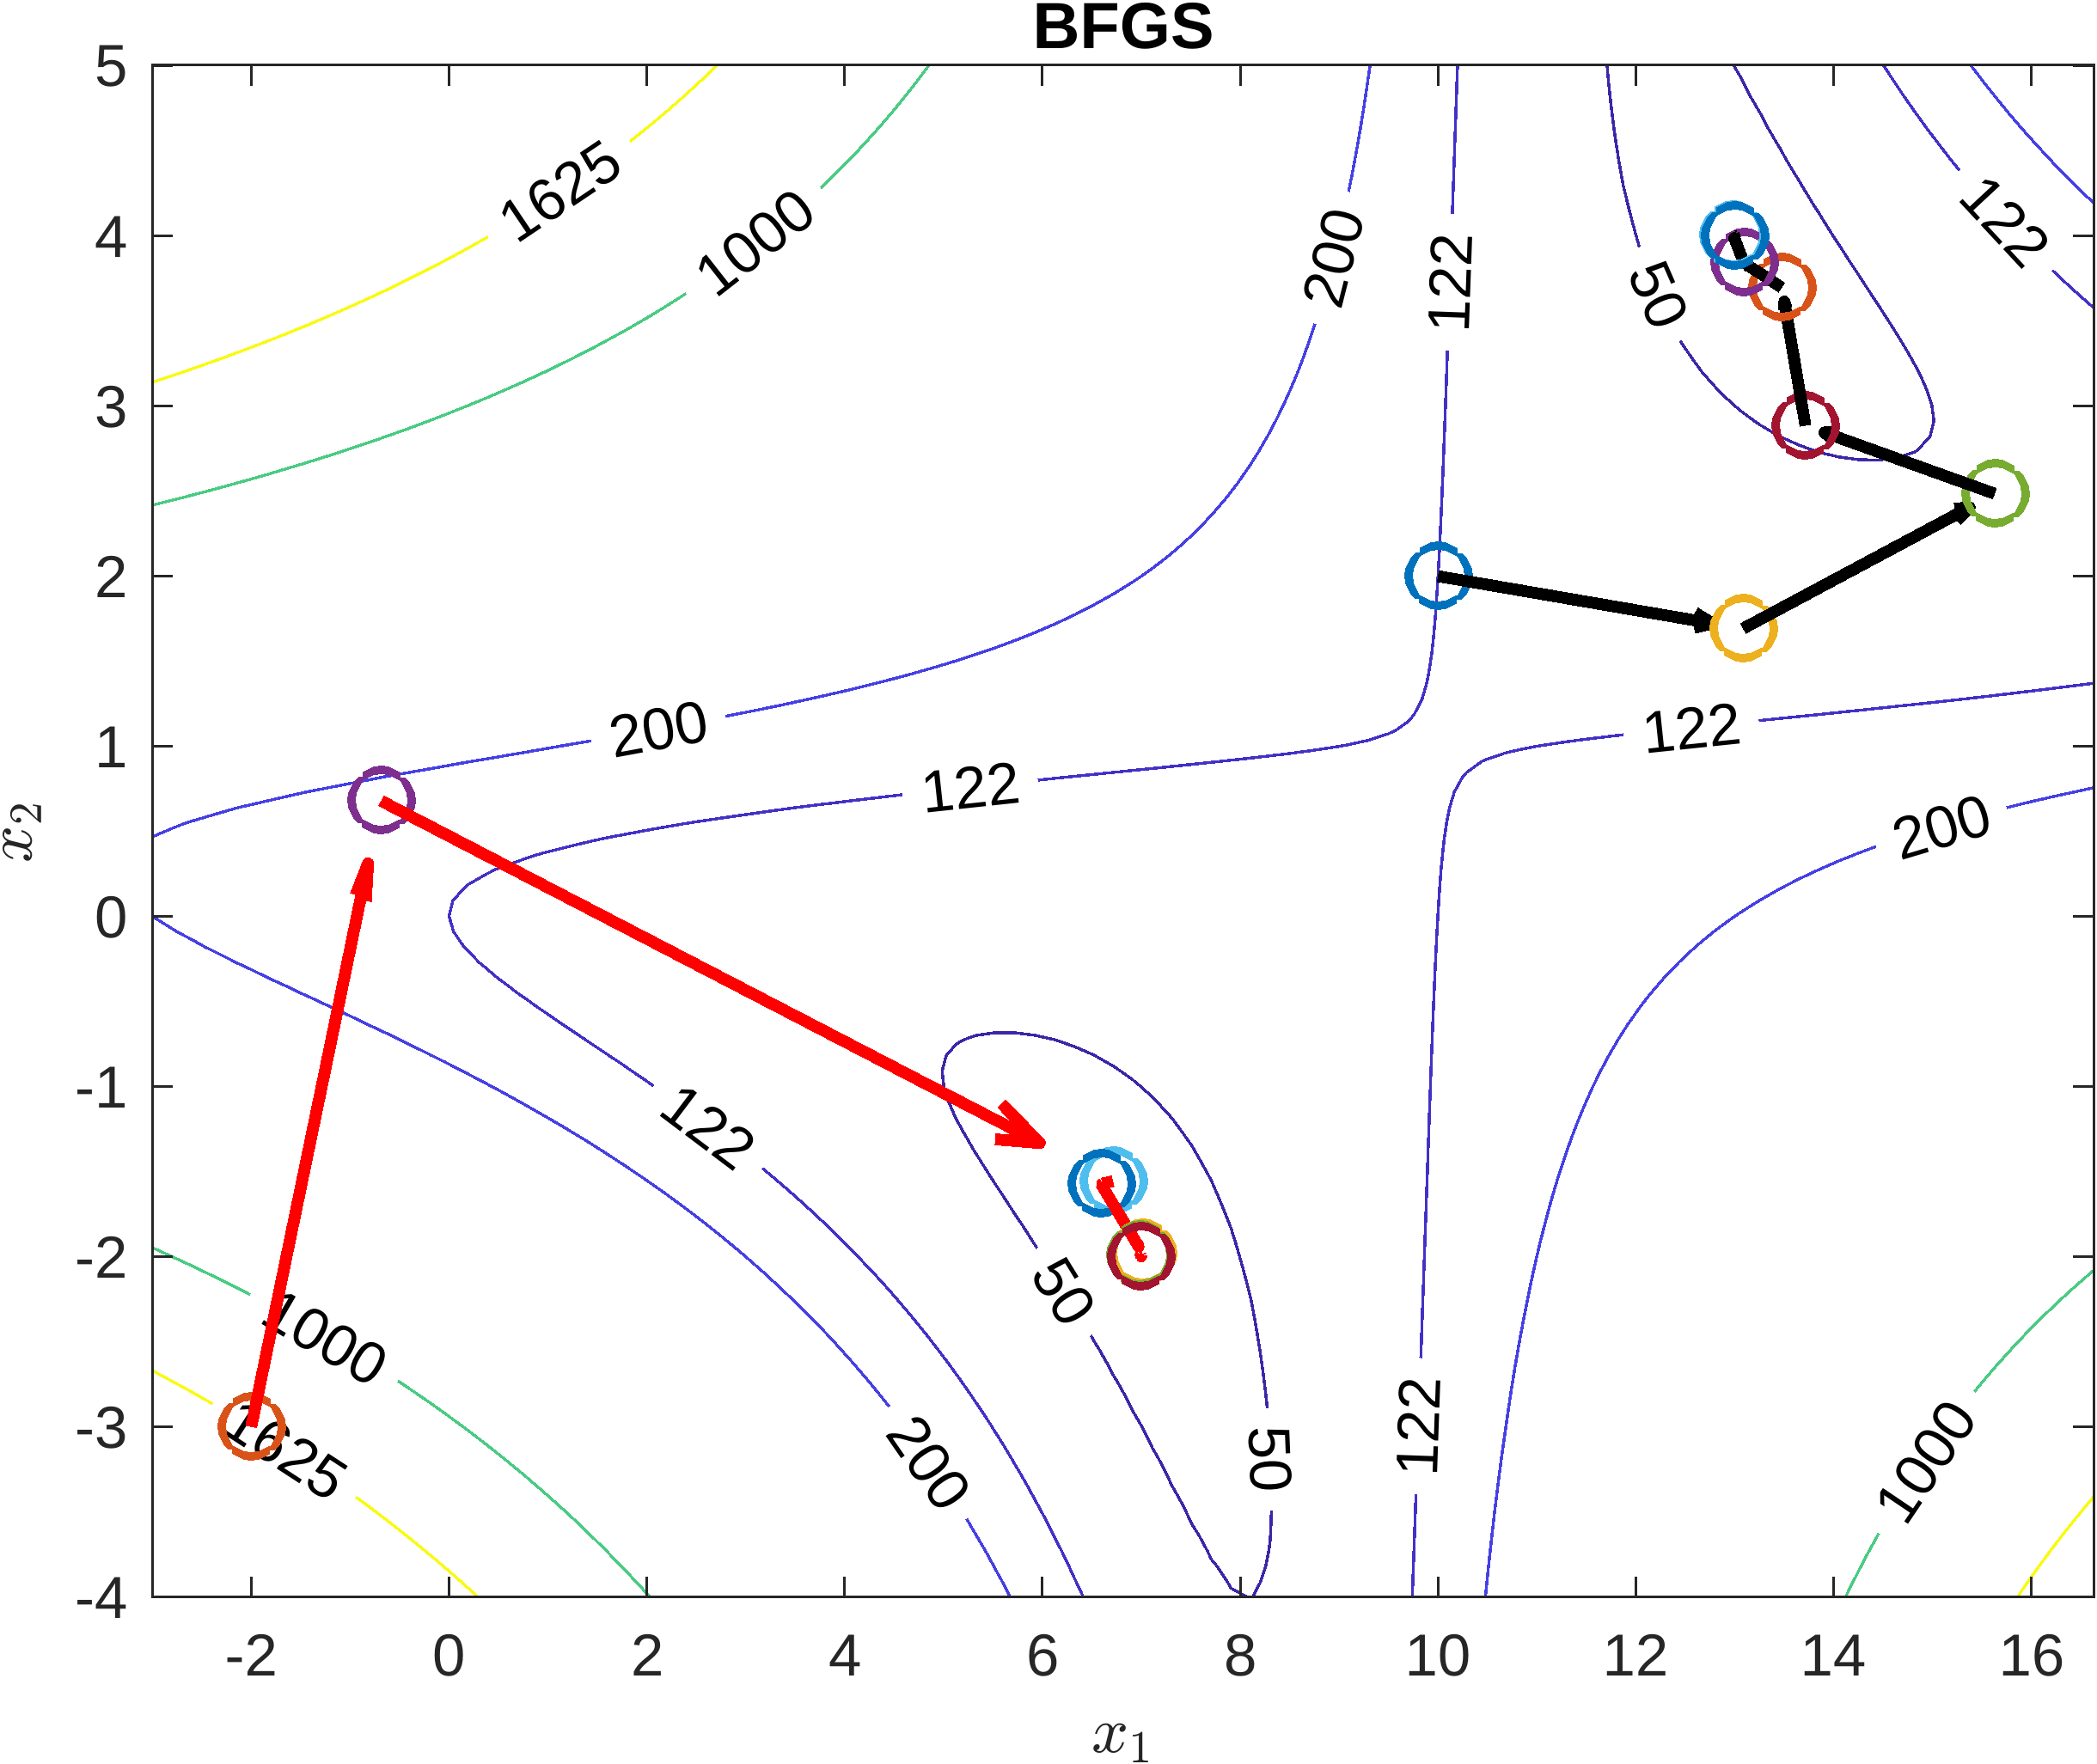
\includegraphics[width=\textwidth]{img01B_m06.png}
            \caption{Curvas de n\'ivel de $f_{1b}$ e pontos $x_{k}$}
            \label{fig:graf01B_m06}
      \end{subfigure}
      \caption{Resultados do m\'etodo BFGS, para as duas fun\c c\~oes e pontos iniciais}
      \label{fig:graf01_m06}
\end{figure}

A tabela \ref{table:resultadosf2} apresenta os principais resultados dos algoritmos implementados para a fun\c c\~ao do item \ref{fun:02}. Al\'em dos pontos de m\'inimo encontrados, as tabelas apresentam tamb\'em o n\'umero de passos para a converg\^encia e o tempo de execu\c c\~ao.

\begin{table}[H]
      \small
      \centering
      \caption{Resultados para a fun\c c\~ao \ref{fun:02}}
      \begin{tabular}{c|c|c|c|c|c}
            m\'etodo           & $x^0$ & $x^{min}$ & passos & $\Delta t$(ms) \\
            \hline
            Univariante         & $\{0.01,-0.10\}^t$     & $\{-0.205,7.789\}^t$  & 11 & 2.1 \\
            Powell              & $\{0.01,-0.10\}^t$     & $\{-0.205,7.789\}^t$  & 12 & 6340.8(**)  \\
            Steepest Descent    & $\{0.01,-0.10\}^t$     & $\{-0.205,7.789\}^t$  &  6 & 0.3 \\
            Flecher-Reeves      & $\{0.01,-0.10\}^t$     & $\{-0.205,7.789\}^t$  & 10 & 0.4 \\
            Newton-Raphson      & $\{0.01,-0.10\}^t$     & $\{-0.205,7.789\}^t$  &  3 & 4.4 \\
            BFGS                & $\{0.01,-0.10\}^t$     & $\{-0.205,7.789\}^t$  &  3 & 0.3 \\
     \end{tabular}
      \label{table:resultadosf2}
\end{table}

No caso da fun\c c\~ao do item \ref{fun:02} nota-se que o elevado tempo de execu\c c\~ao do m\'todo de Powell (**) em rela\c c\~ao aos demais.

A figuras \ref{fig:graf02_ordem0}, \ref{fig:graf02_ordem1} e \ref{fig:graf02_ordem2} a seguir ilustram, para os seis m\'etodos, as curvas de n\'ivel de $f$ para os casos da fun\c c\~ao do item \ref{fun:02}, bem como a trajet\'oria dos pontos $\vec{x_{k}}$ associadoas ao algoritmo de minimiza\c c\~ao.

\begin{figure}[H]
      \centering
      \begin{subfigure}{0.45\textwidth}
            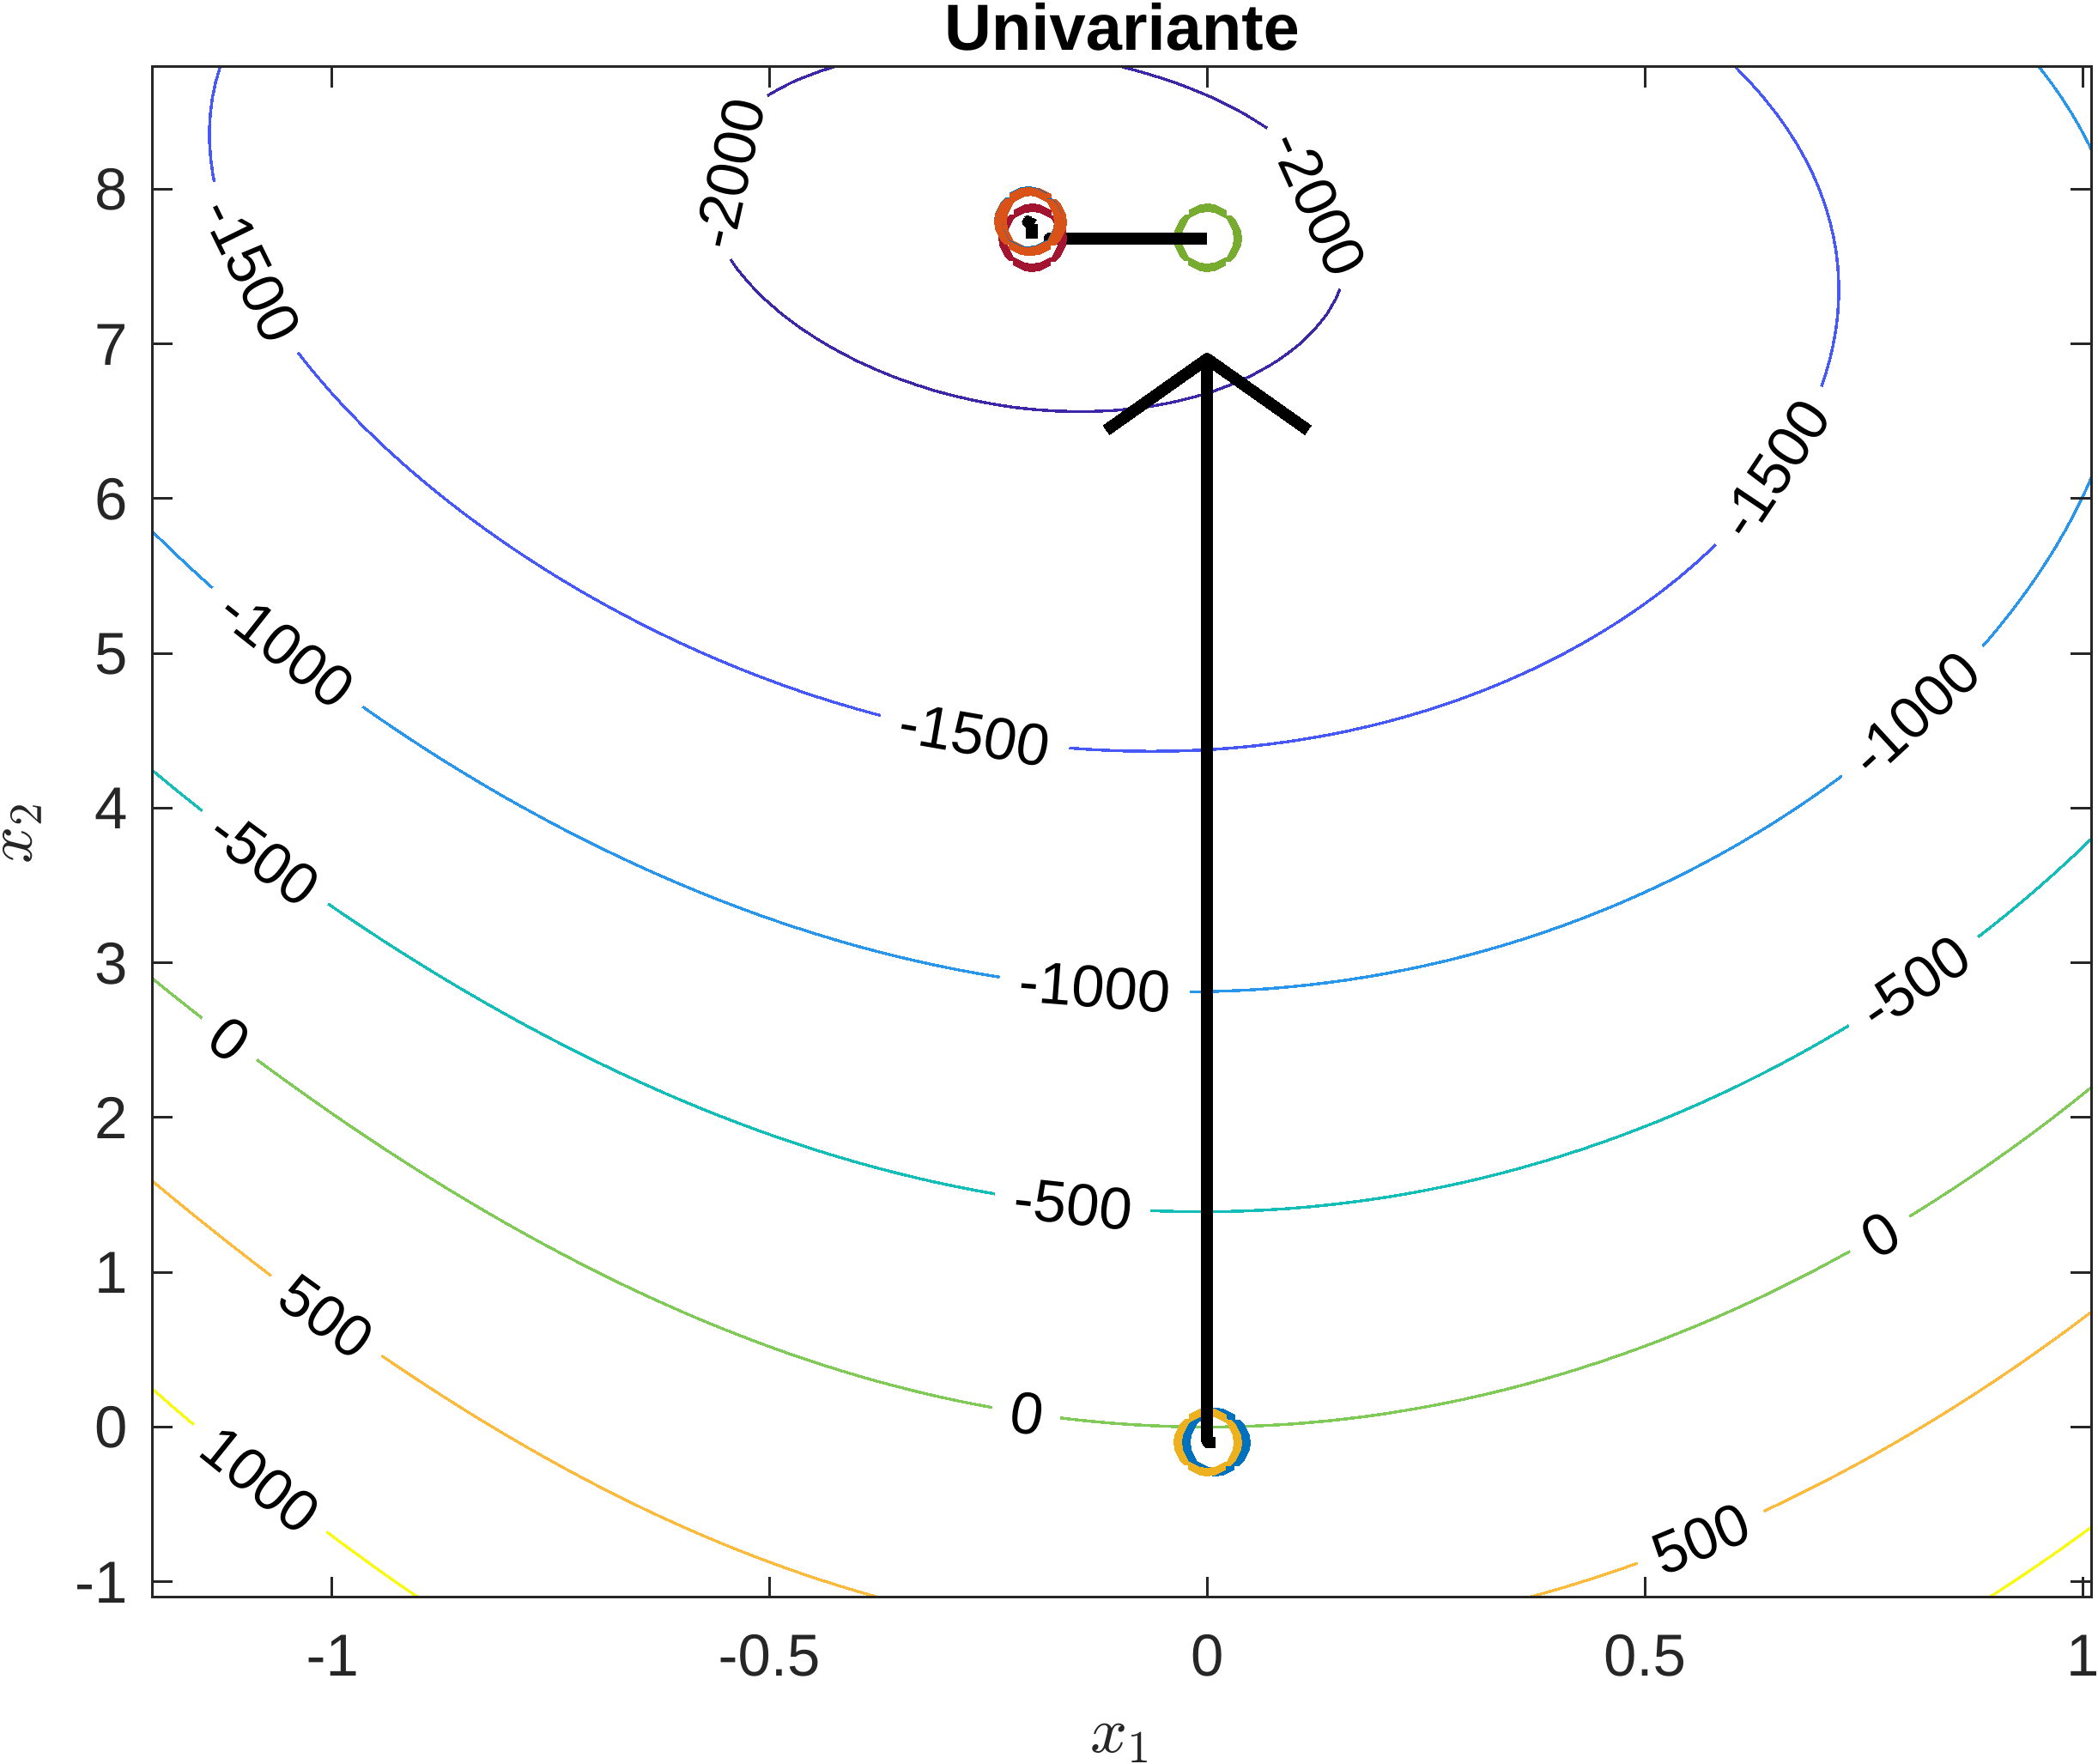
\includegraphics[width=\textwidth]{img02_m01.png}
            \caption{Univariante}
            \label{fig:graf02_m01}
      \end{subfigure}
      \begin{subfigure}{0.45\textwidth}
            \centering
            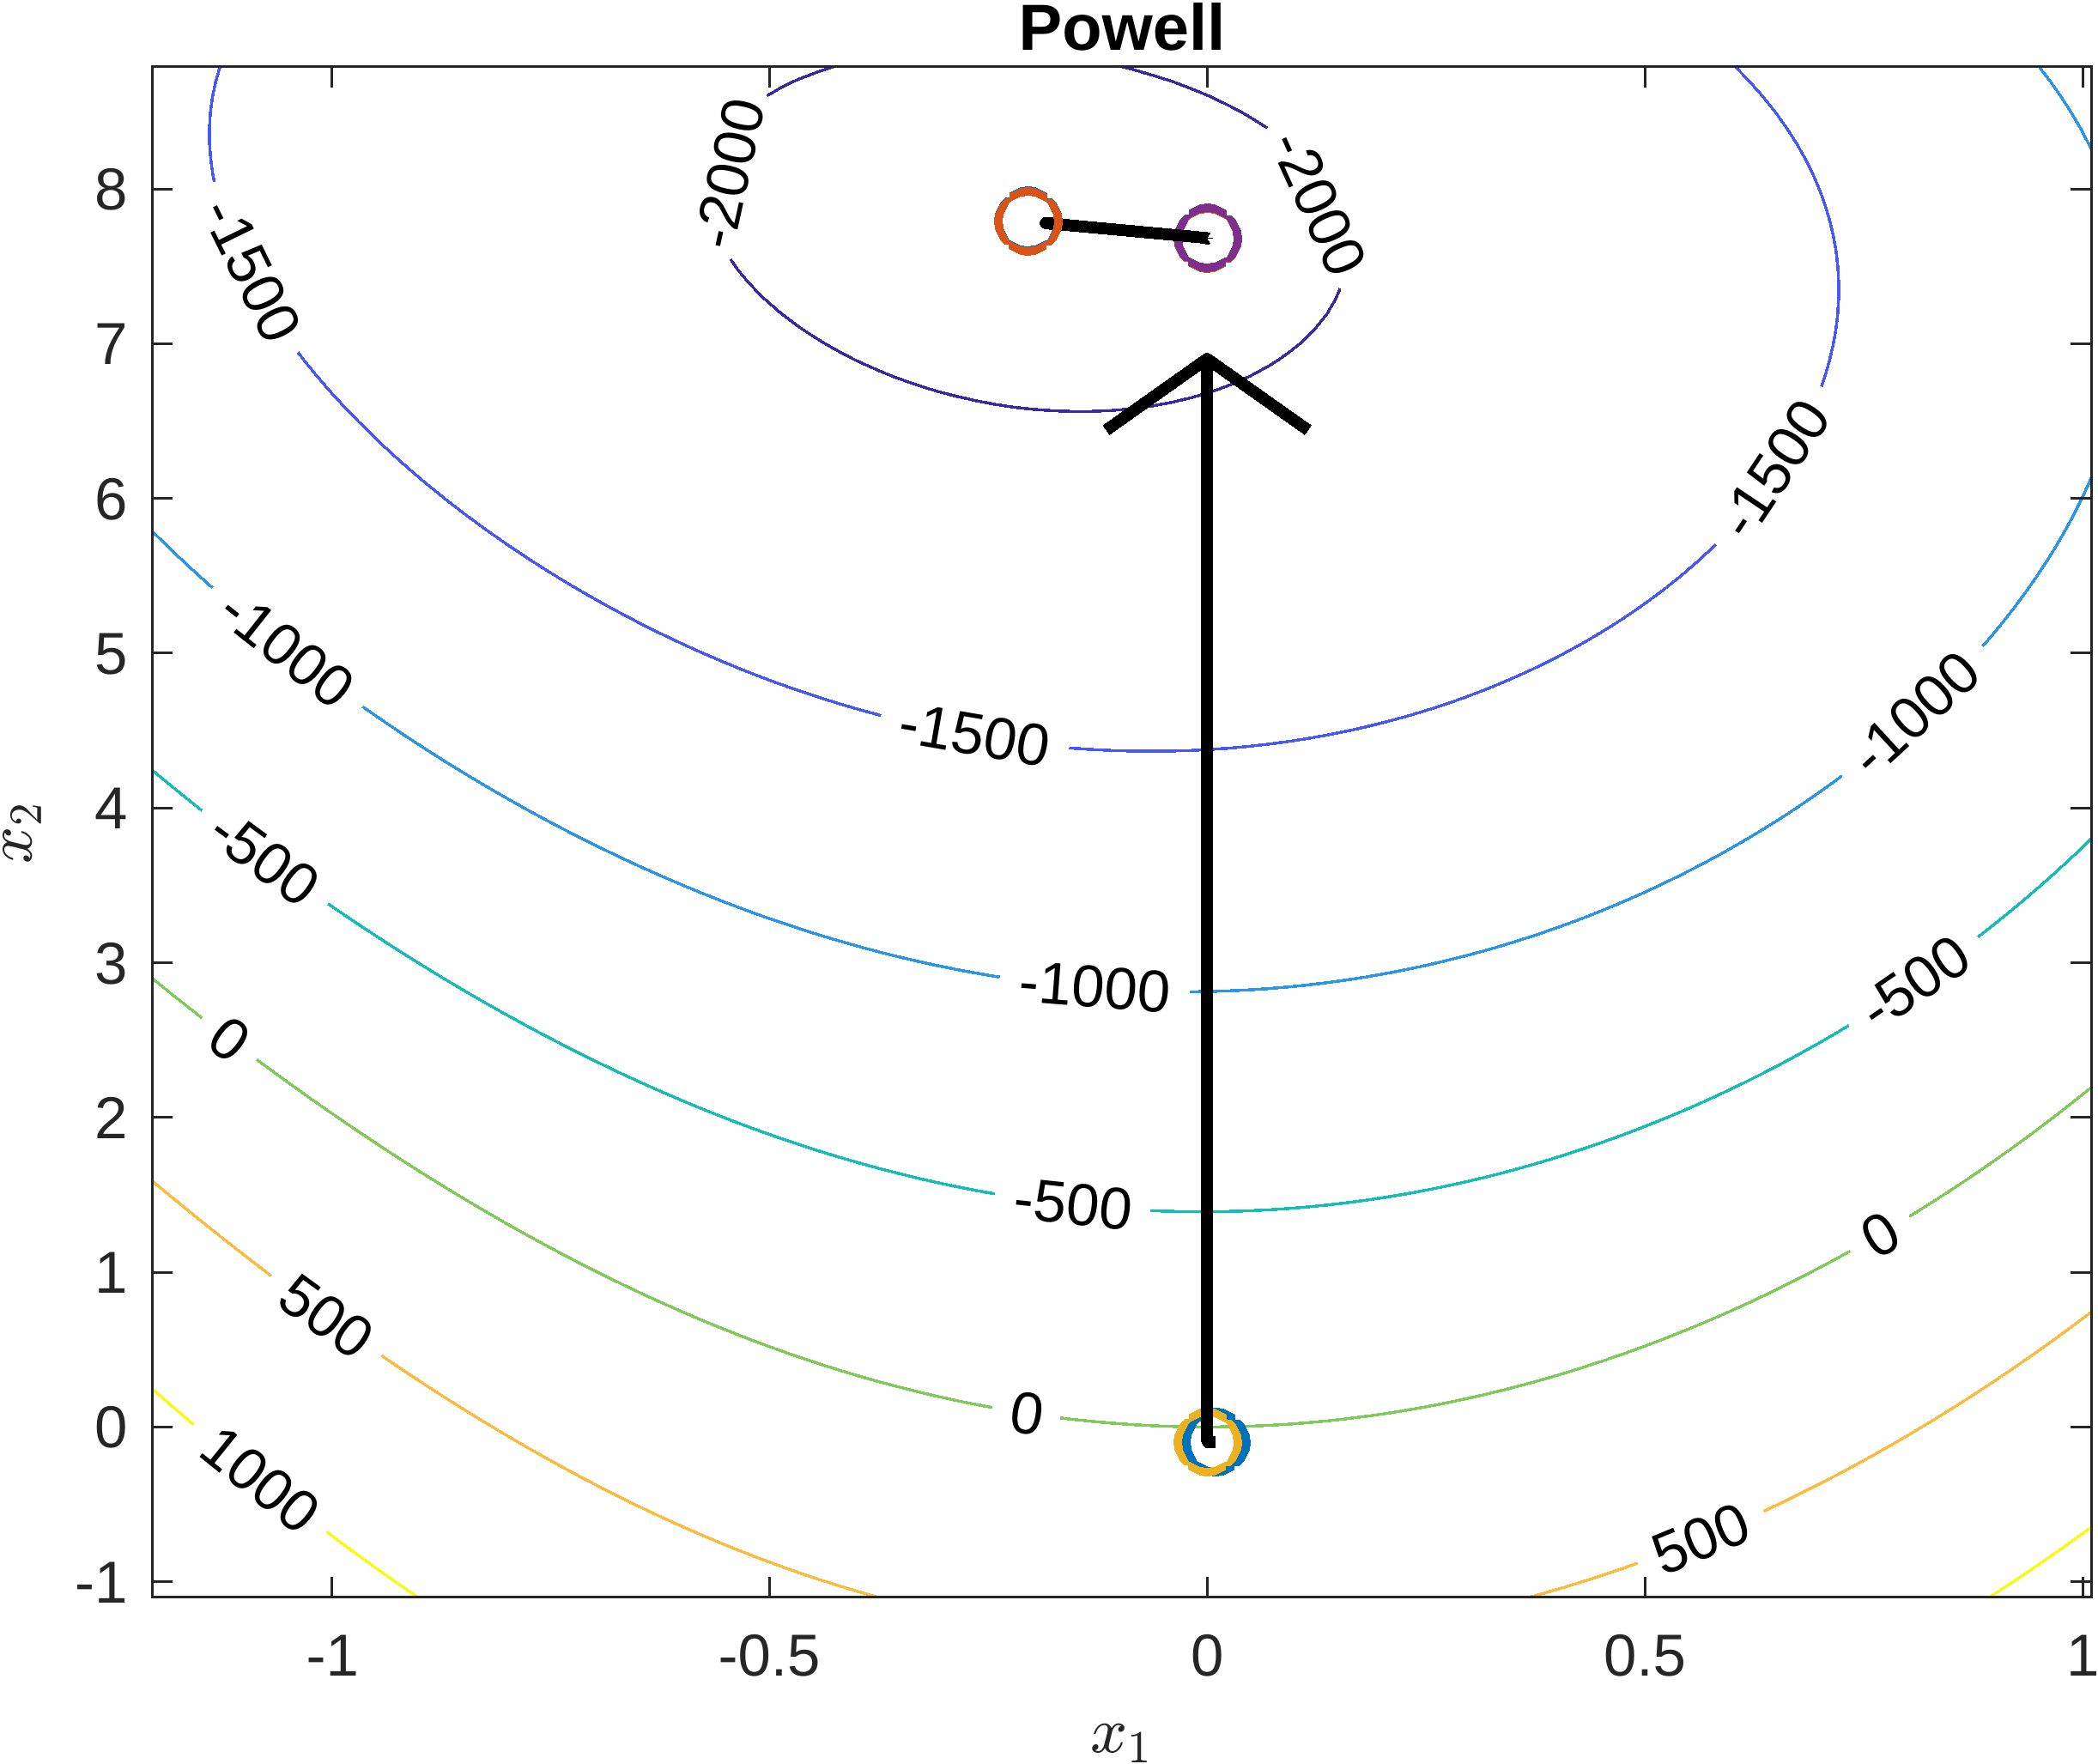
\includegraphics[width=\textwidth]{img02_m02.png}
            \caption{Powell}
            \label{fig:graf02_m02}
      \end{subfigure}
      \caption{Curvas de n\'ivel de $f_{2}$ e pontos $x_{k}$, m\'etodos de ordem zero}
      \label{fig:graf02_ordem0}
\end{figure}

\begin{figure}[H]
      \centering
      \begin{subfigure}{0.45\textwidth}
            \centering
            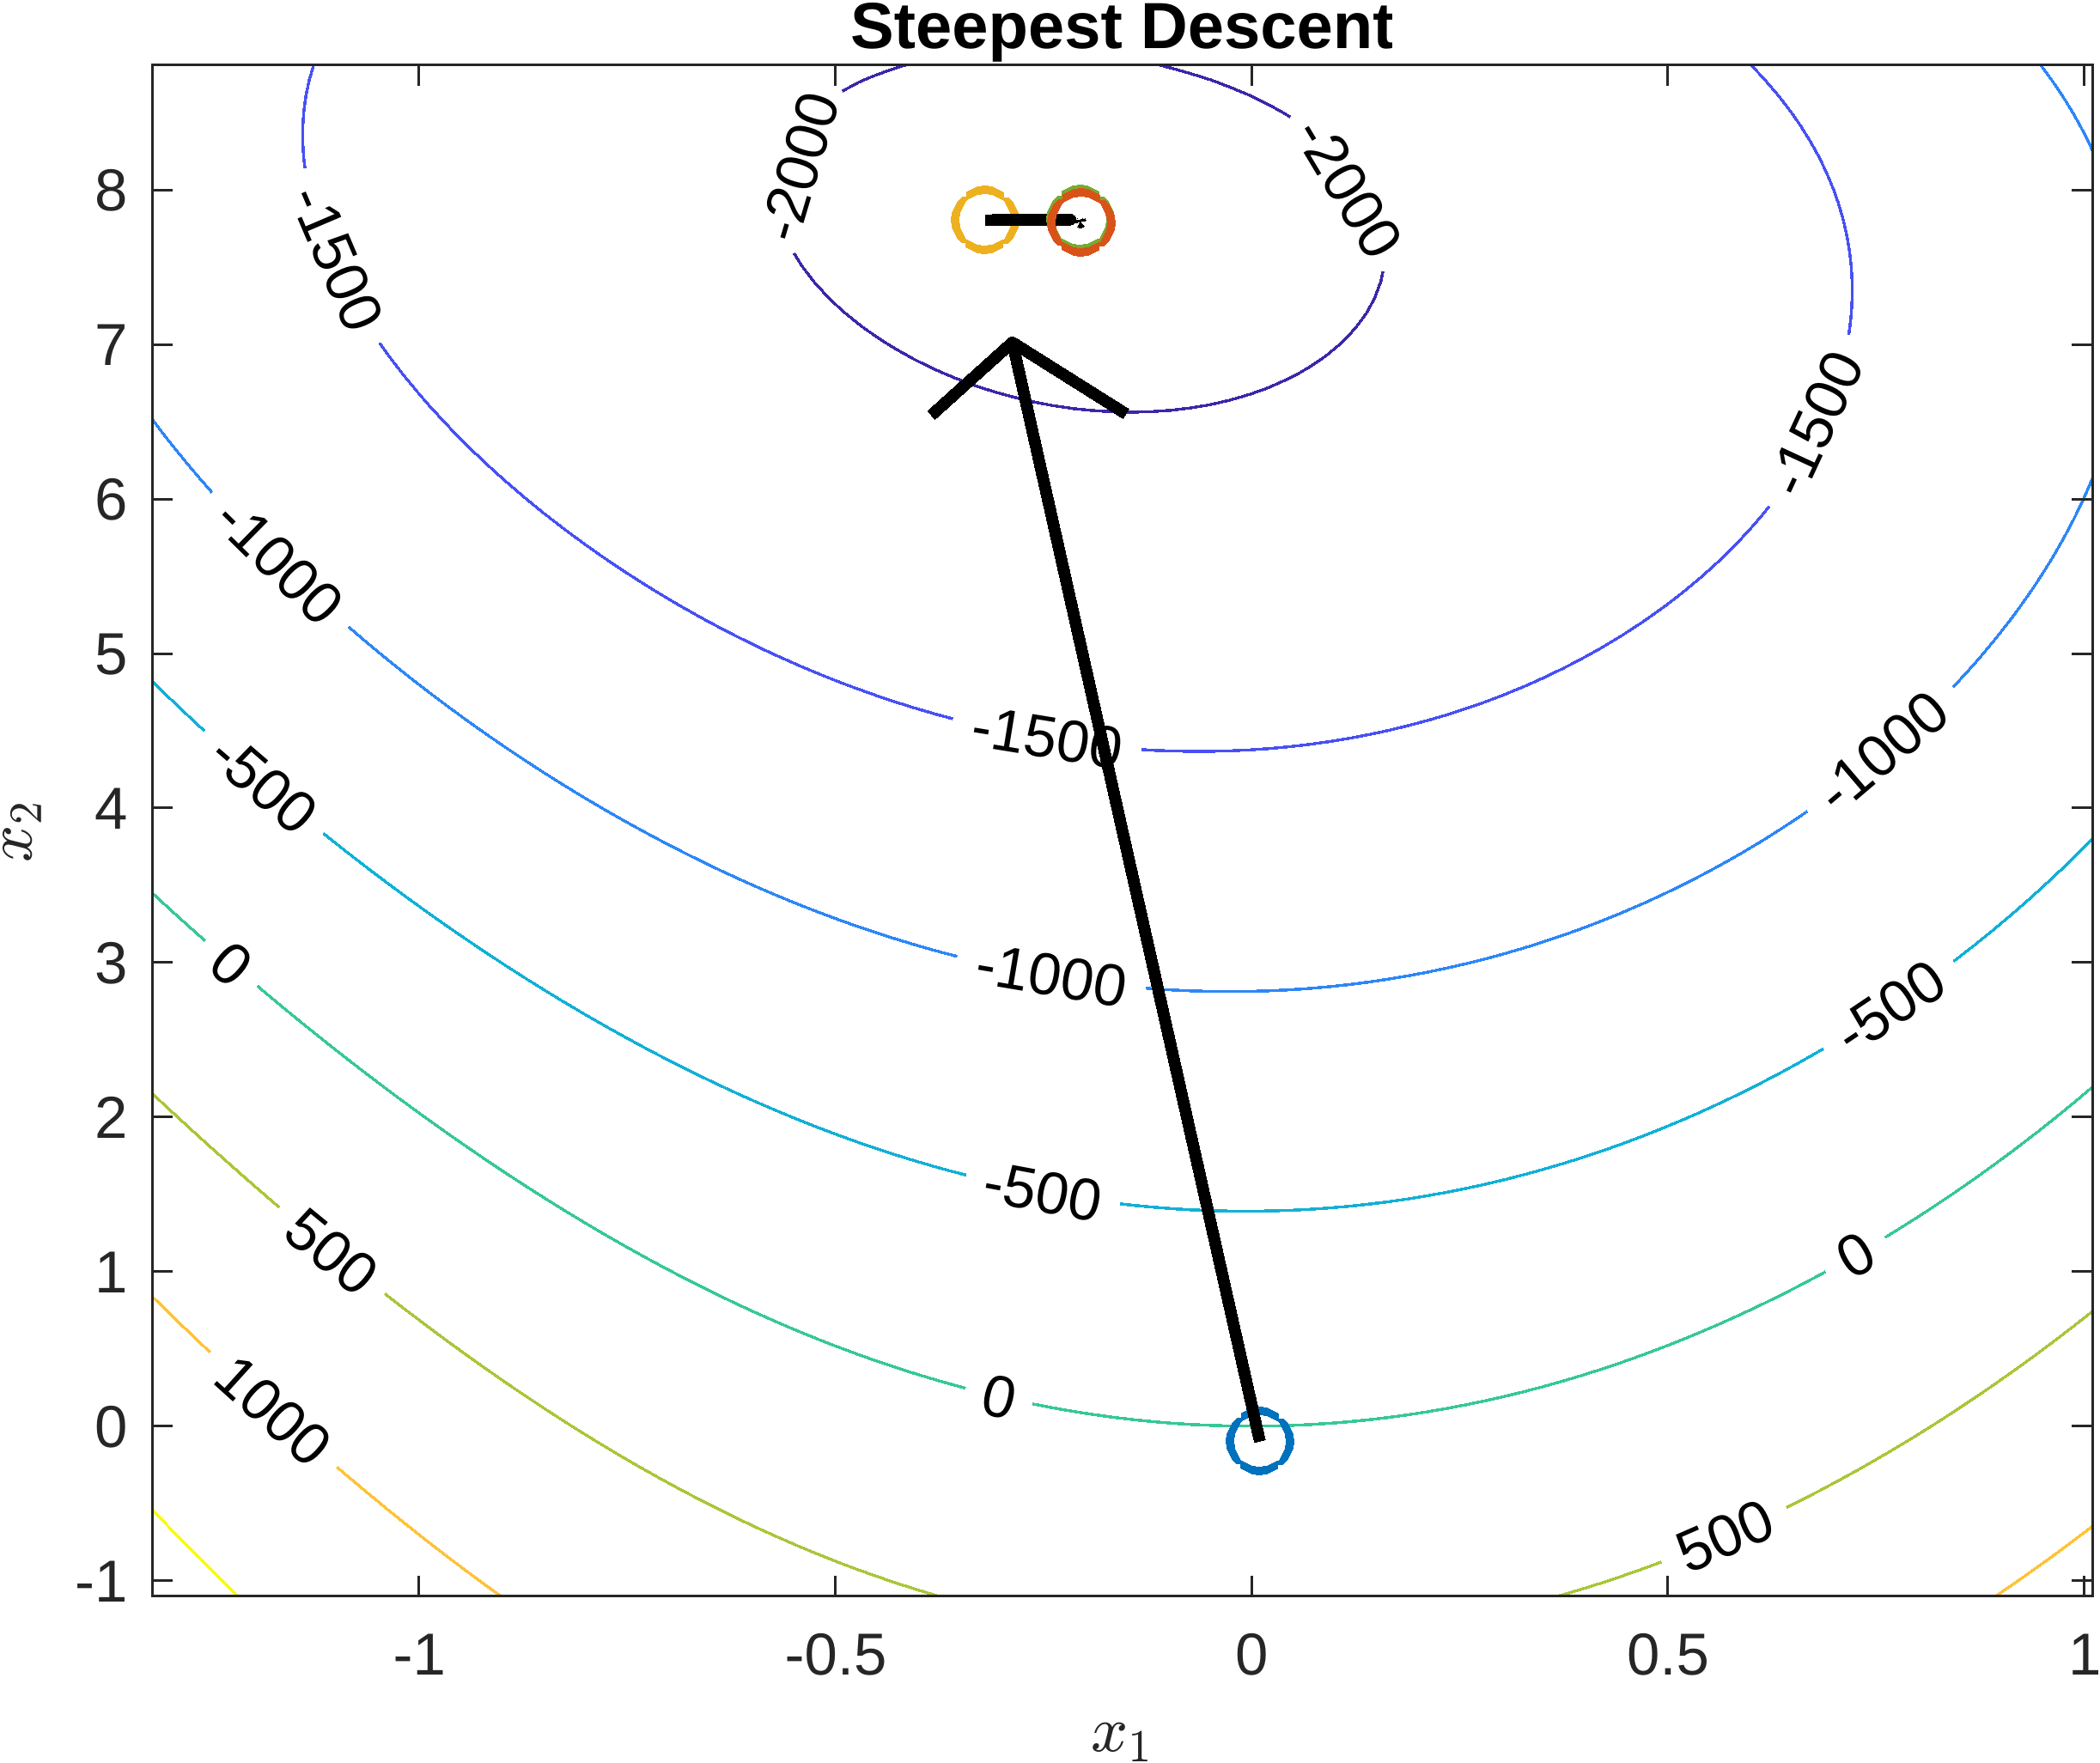
\includegraphics[width=\textwidth]{img02_m03.png}
            \caption{Steepest Descent}
            \label{fig:graf02_m03}
      \end{subfigure}
      \begin{subfigure}{0.45\textwidth}
            \centering
            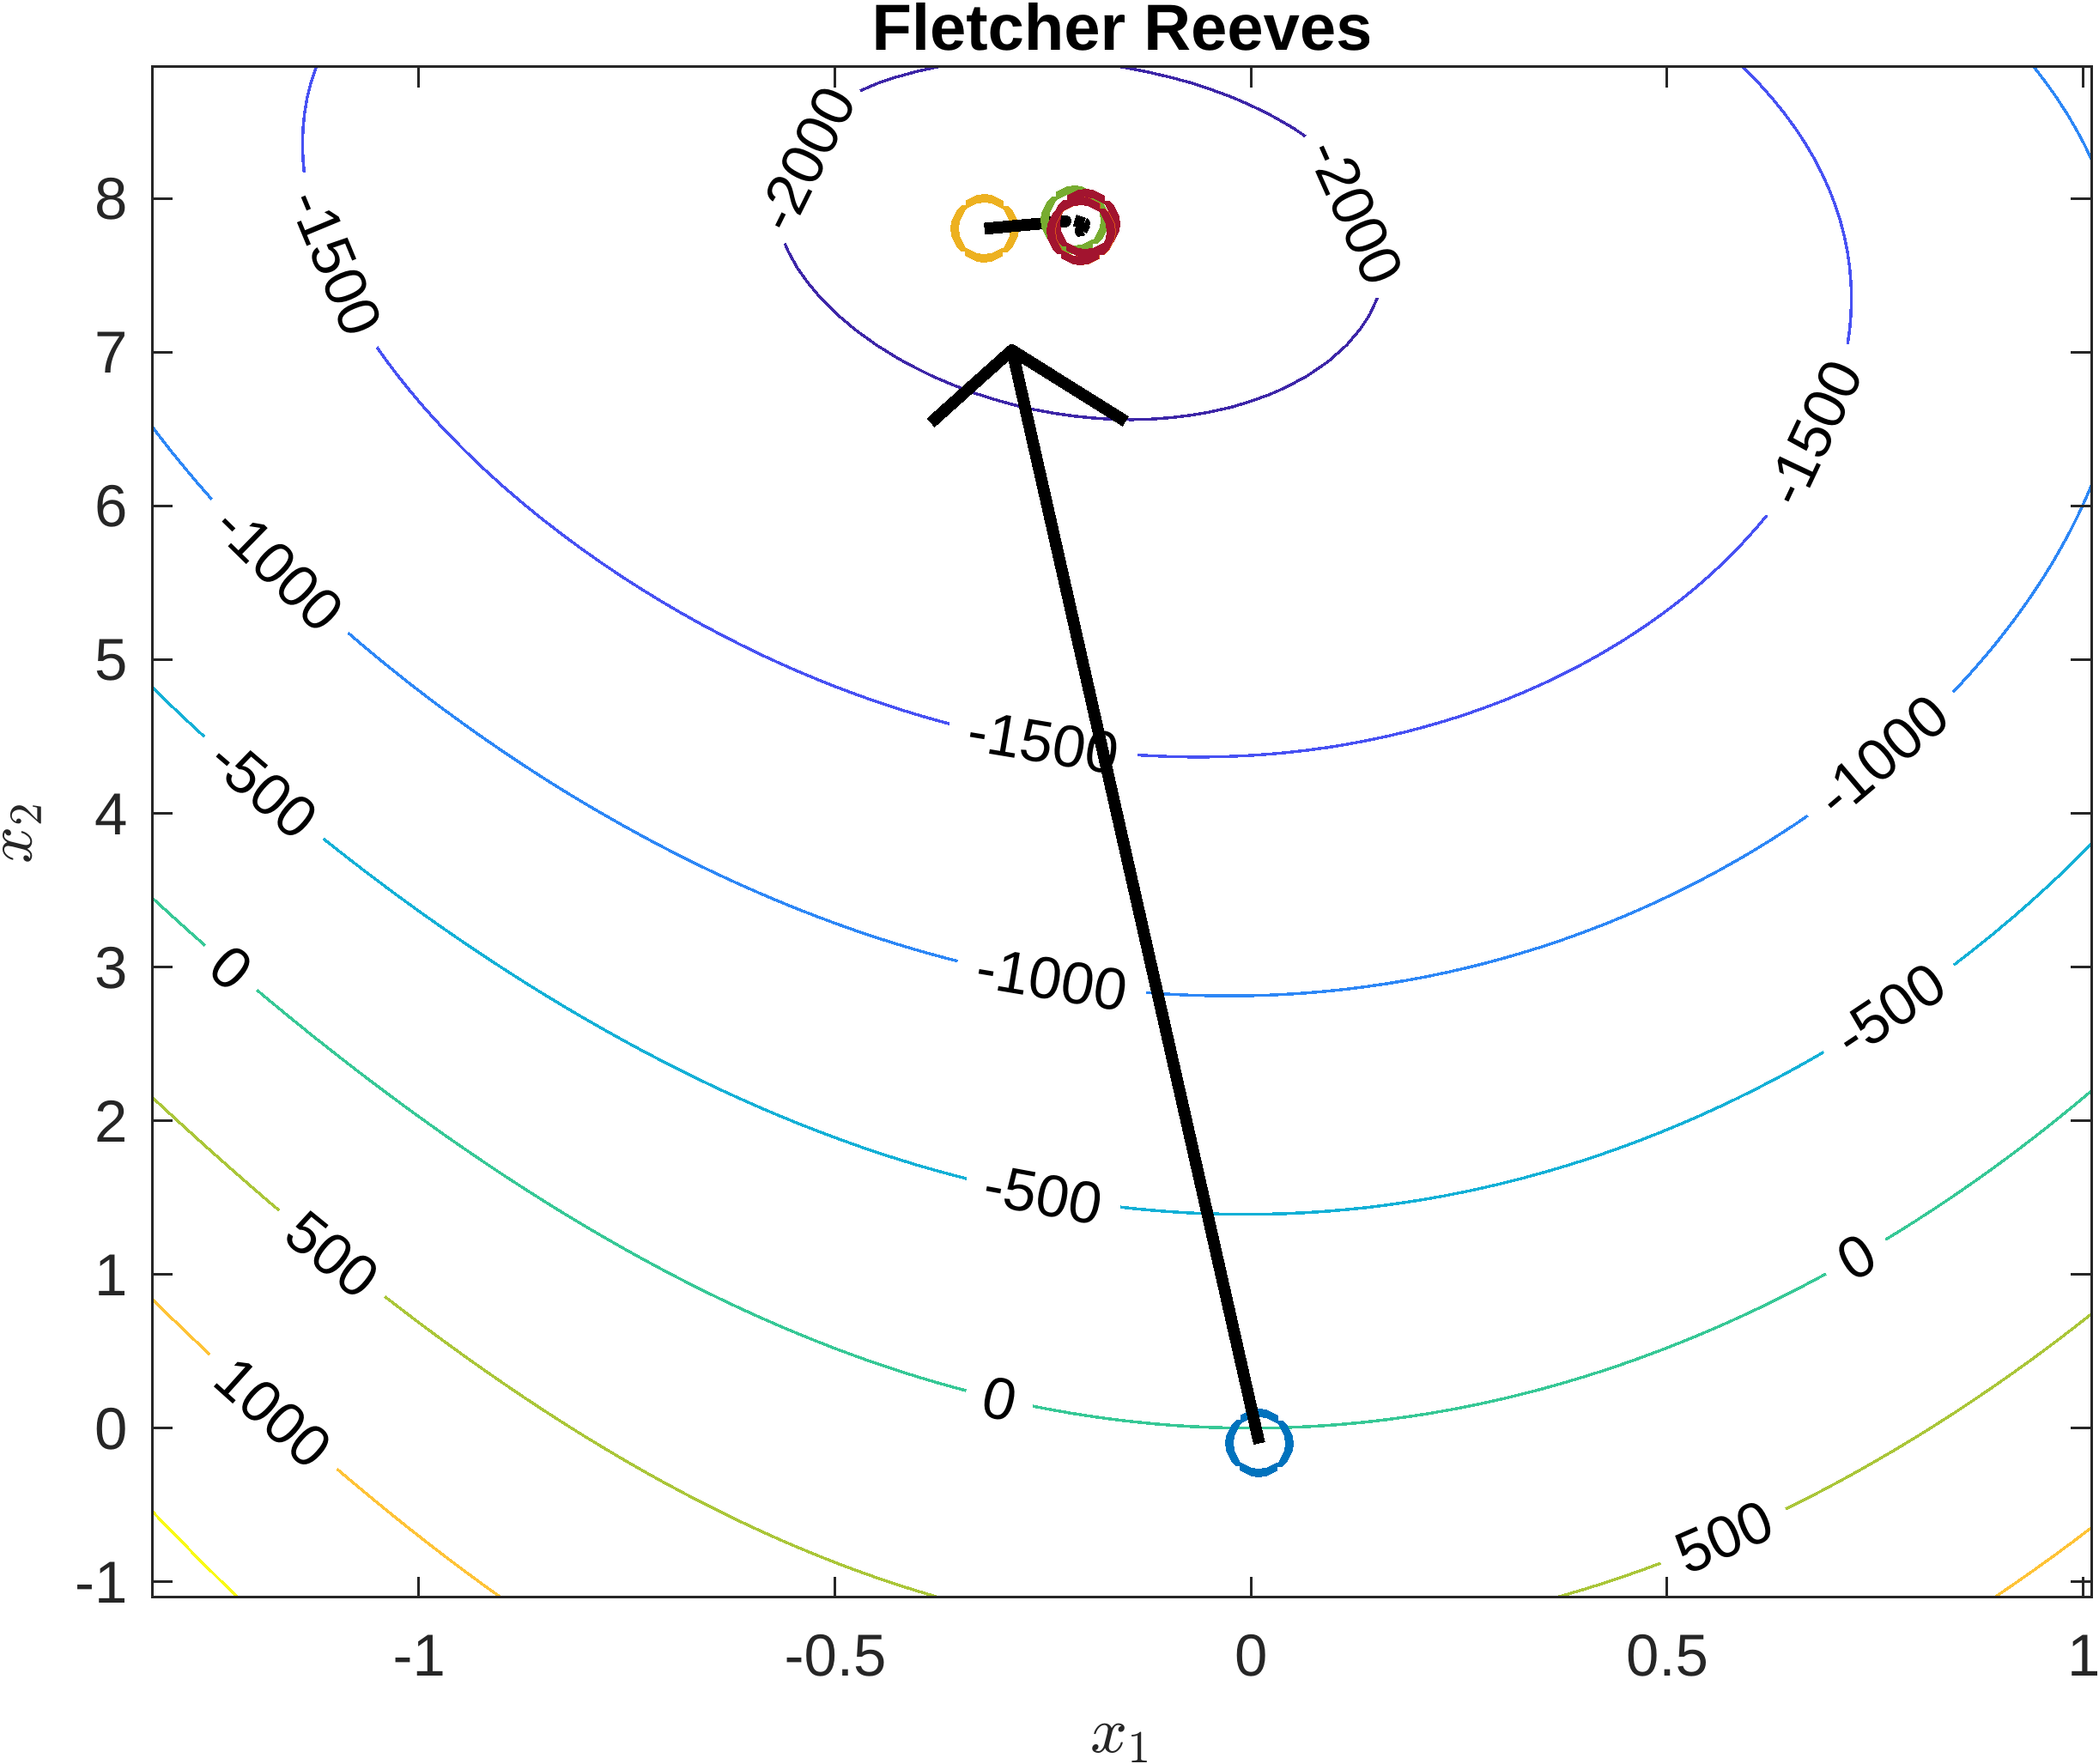
\includegraphics[width=\textwidth]{img02_m04.png}
            \caption{Flecher-Reeves}
            \label{fig:graf02_m04}
      \end{subfigure}
      \caption{Curvas de n\'ivel de $f_{2}$ e pontos $x_{k}$, m\'etodos de ordem um}
      \label{fig:graf02_ordem1}
\end{figure}

\begin{figure}[H]
      \centering
      \begin{subfigure}{0.45\textwidth}
            \centering
            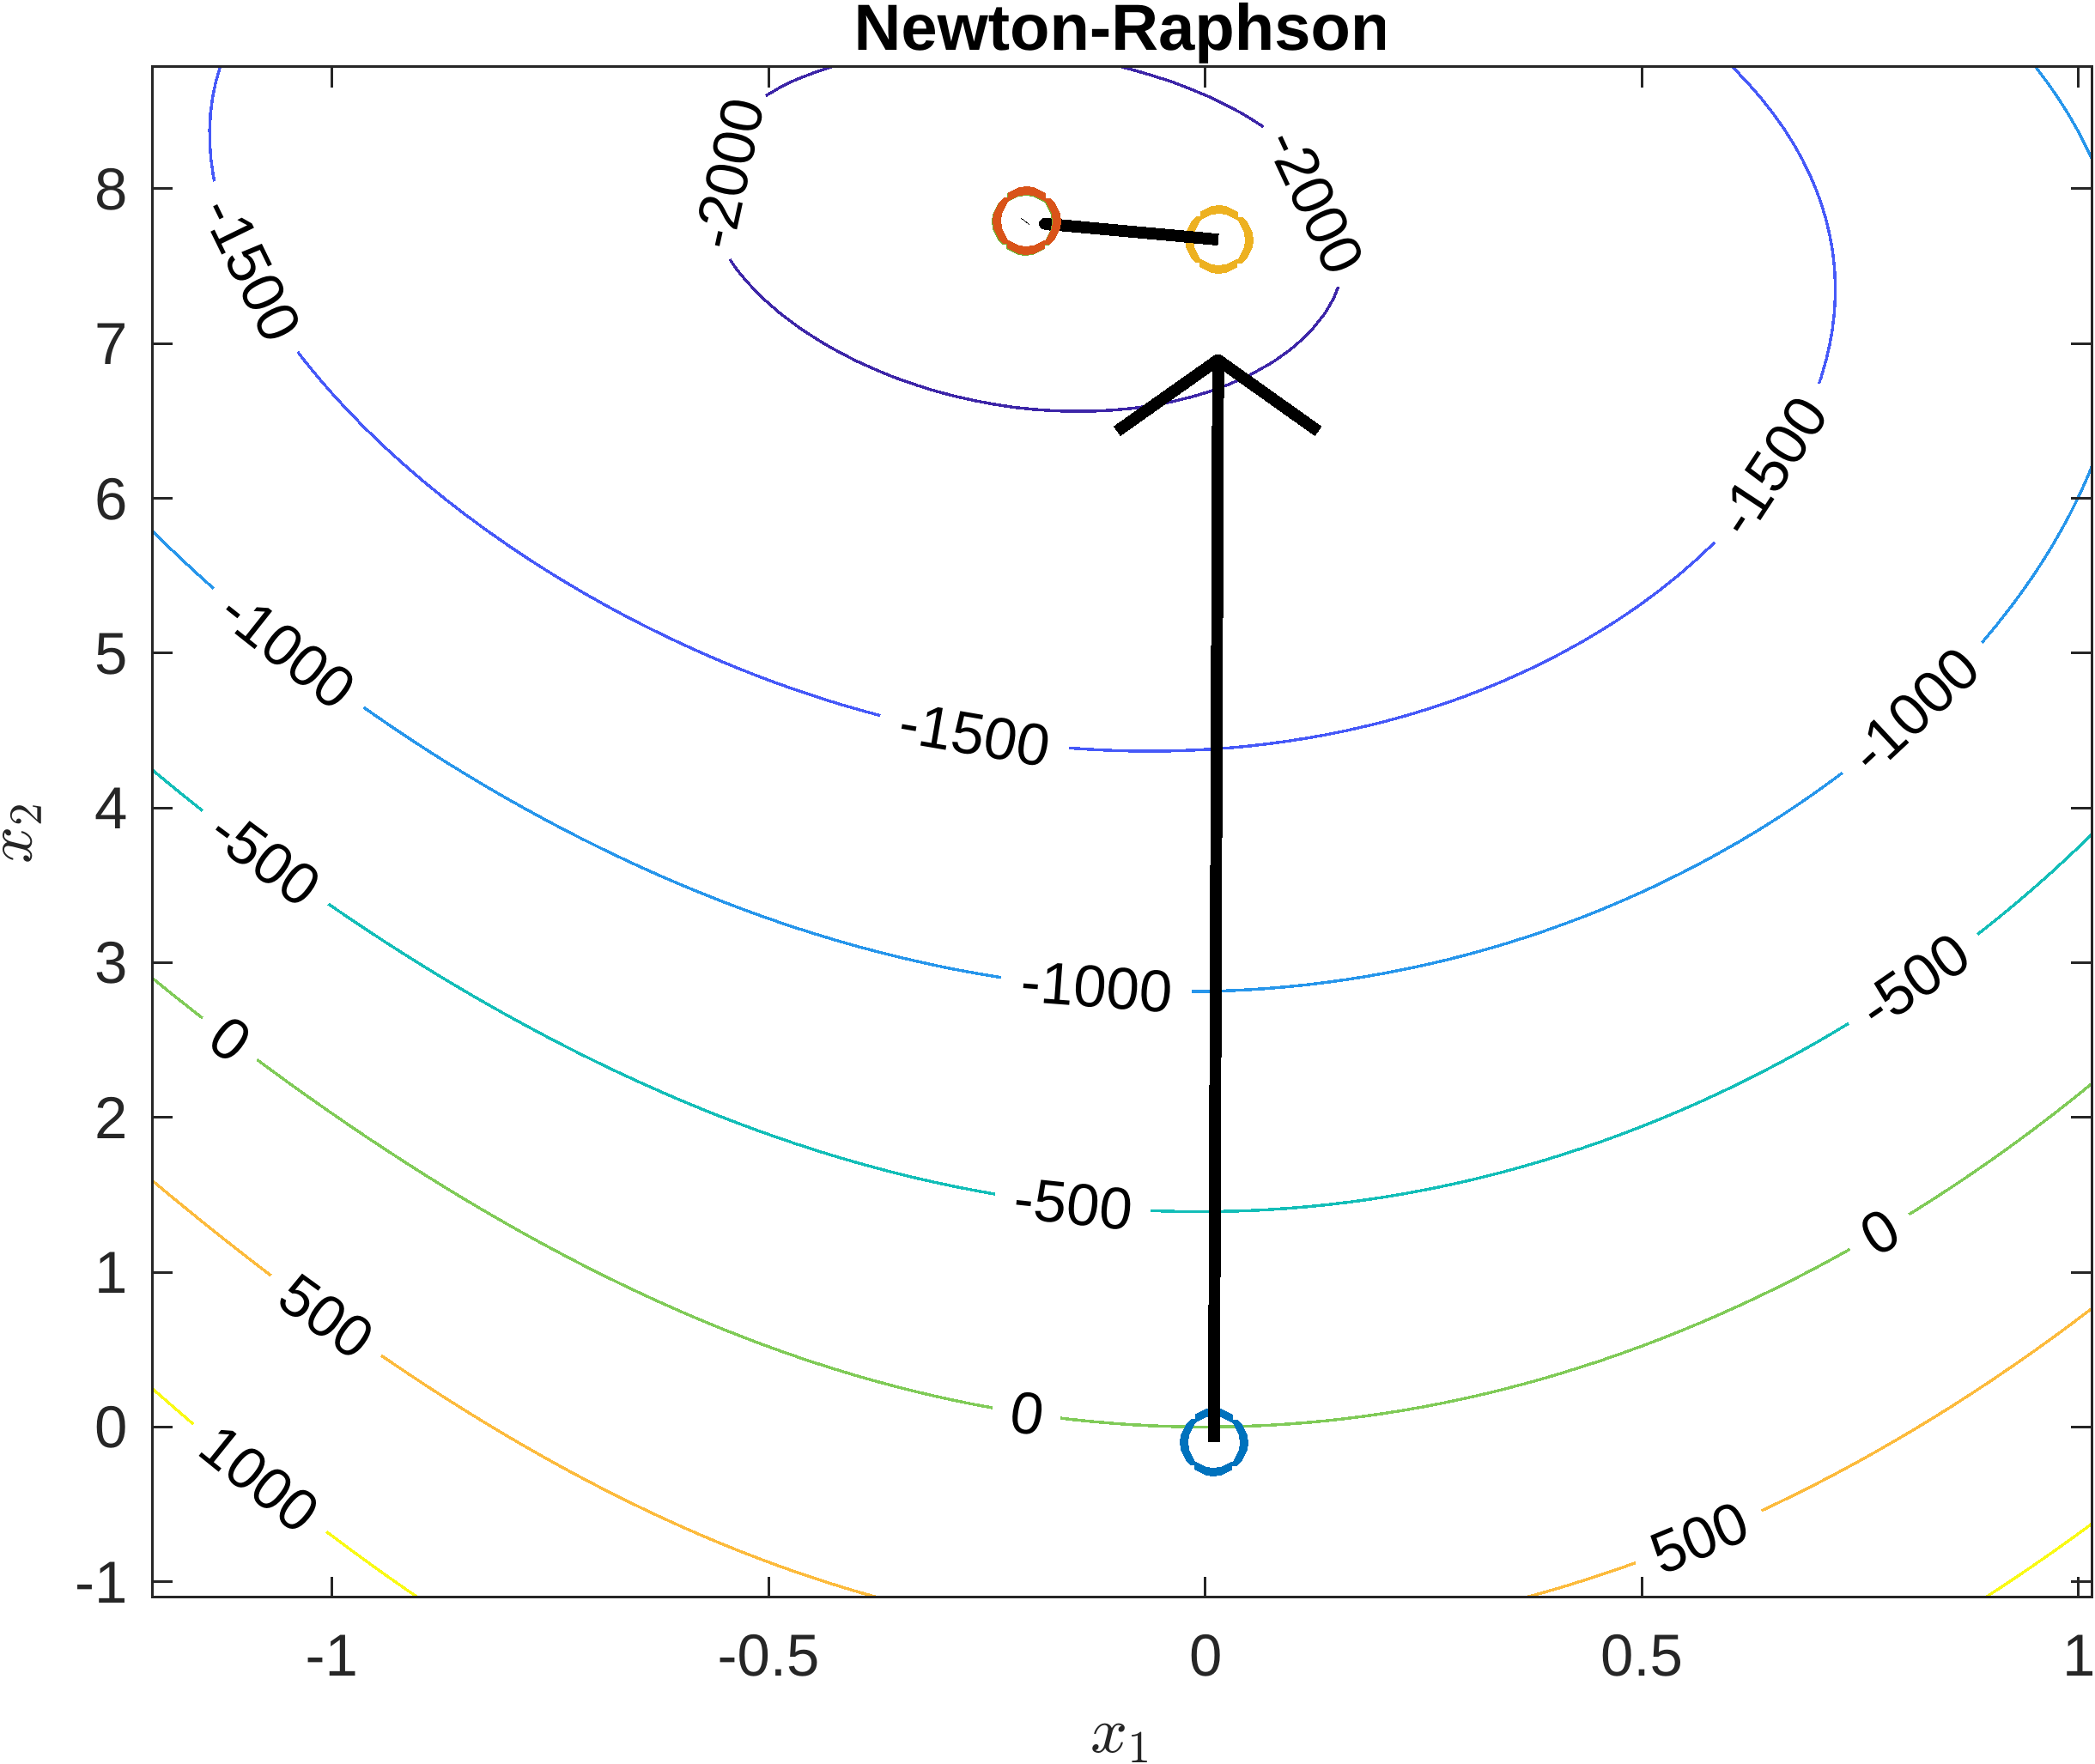
\includegraphics[width=\textwidth]{img02_m05.png}
            \caption{Newton-Raphson}
            \label{fig:graf02_m05}
      \end{subfigure}
      \begin{subfigure}{0.45\textwidth}
            \centering
            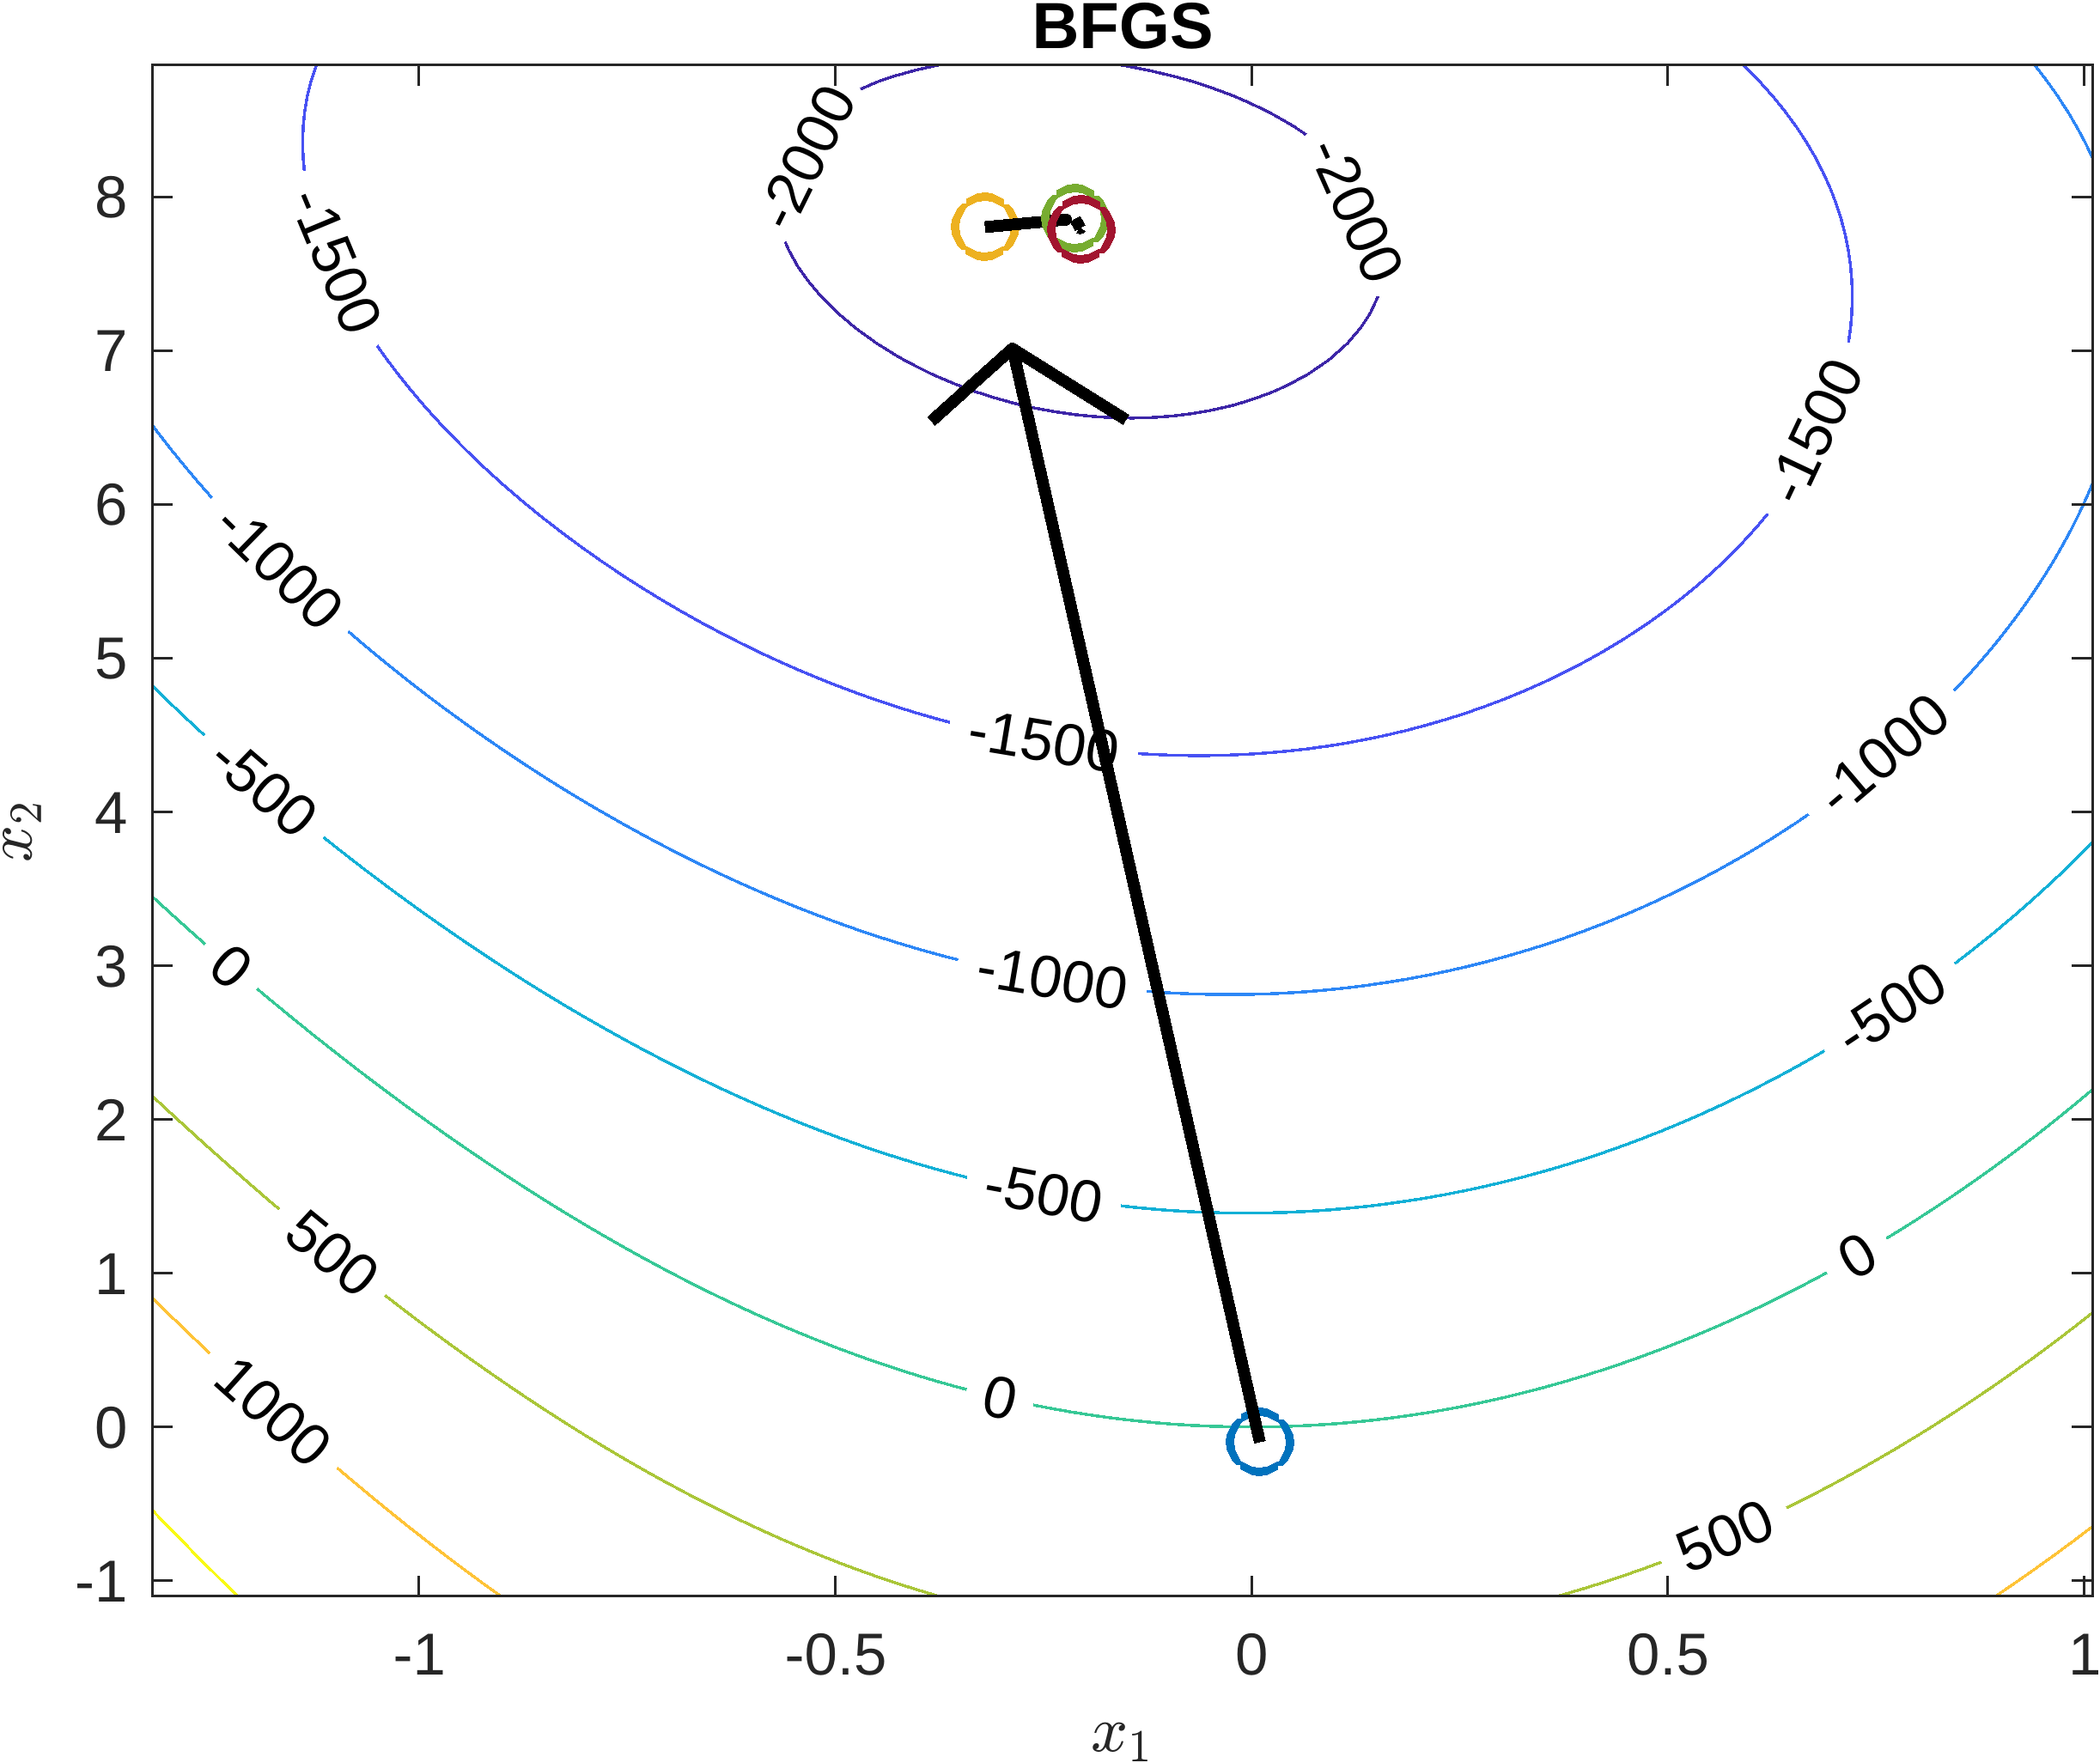
\includegraphics[width=\textwidth]{img02_m06.png}
            \caption{BFGS}
            \label{fig:graf02_m06}
      \end{subfigure}
      \caption{Curvas de n\'ivel de $f_{2}$ e pontos $x_{k}$, m\'etodos de Newton-Rapshon e BFGS}
      \label{fig:graf02_ordem2}
\end{figure}

\section{Conclus\~oes}

A realiza\c c\~ao deste trabalho permitiu implementar os m\'etodos estudados na disciplina de otimiza\c c\~ao. Para todos os casos de aplica\c c\~ao, foram rodados os algortimos para outros pontos que n\~ao os pontos propostos no problema em si e cujo resultado mostrou que os algortimos de busca e miniza\c c\~ao s\~ao robustos, mesmo nos casos de fun\c c\~oes n\~ao quadr\'aticas.

Em alguns poucos casos o algoritmo n\~ao obteve o resultado esperado, seja o n\'umero de passos at\'e a converg\^encia ou a converg\^encia em si n\~ao ter sido atingida. Em geral, notou-se que a converg\^encia, n\'umero de passos e o tempo de execu\c c\~ao dos algoritmos \'e muito sens\'ivel a escolha de seus par\^metros, o que reside nas incertezas num\'ericas associadas aos m\'etodos de busca linear, principalmente.

\section{Anexos}

A seguir est\~ao ilustrados alguns dos c\'odigos ou trechos de c\'odigos decritos na metodologia.

\begin{minipage}{\linewidth}
      \begin{lstlisting}[style=myStyle, caption=script t01.m setando par\^ametros e criando as fun\c c\~oes, label=l1]
            % dados do item 01a, f, grad f, hess f e x0
            fa = @(x) x(1)^2-3*x(1)*x(2)+4*x(2)^2+x(1)-x(2);
            gfa = @(x) [2*x(1)-3*x(2)+1 ; -3*x(1)+8*x(2)-1];
            Ha = @(x) [2 -3;-3 8];
            x01 = [2;2];
            x02 = [-1;-3];
            % parametros dos algoritmos
            iter_max = 100;
            a = 0.002; % passo
            TOL = 1e-4; % parada do gradiente
            TOL2 = 1e-7; % busca linear
            methods = ["Univariante","Powell","Steepest Descent","Fletcher Reeves","Newton-Raphson","BFGS"];
      \end{lstlisting}
\end{minipage}

\begin{minipage}{\linewidth}
      \begin{lstlisting}[style=myStyle, caption=script t01.m chamando o script osr.m para a fun\c c\~ao do item 1a para cada um dos 6 m\'etodos estudados, label=l2]
            fprintf('\n******************** ITEM 01A ************************\n');
            for method = 1:6
                fprintf('---%s---\n', methods(method));

                fprintf('x0=[%2d,%2d]: ',x01(1), x01(2));
                [x_1,t] = osr (fa, gfa, Ha, x01, method, iter_max, a, TOL, TOL2);
                fprintf('(%.1fms), xmin=[%0.4f,%0.4f], f=%0.4f\n', t*1000, x_1(1,end), x_1(2,end), fa(x_1(:,end)));

                fprintf('x0=[%2d,%2d]: ',x02(1), x02(2));
                [x_2,t] = osr (fa, gfa, Ha, x02, method, iter_max, a, TOL, TOL2);
                fprintf('(%.1fms), xmin=[%0.4f,%0.4f], f=%0.4f\n', t*1000, x_2(1,end), x_2(2,end), fa(x_2(:,end)));

                plot_result(min([x_1(1,:), x_2(1,:)])-dx,max([x_1(1,:), x_2(1,:)])+dx,min([x_1(2,:), x_2(2,:)])-dx,max([x_1(2,:), x_2(2,:)])+dx, x_1, x_2, methods(method), 1)
                exportgraphics(gcf,strcat('./figures/img01A_m0',num2str(method),'.png'),'Resolution',500)
            end
      \end{lstlisting}
\end{minipage}

\begin{minipage}{\linewidth}
      \begin{lstlisting}[style=myStyle, caption=script osr.m implementando o m\'etodo de Powell, label=list_osr]
            function [x_,time_elap] = osr (f, gf, H, x0, method, iter_max, a, TOL, TOL2)
            % 1. Univariante
            % 2. Powell
            % 3. Steepest Descent
            % 4. Flecher?Reeves
            % 5. Newton?Raphson
            % 6. BFGS

            k=0;
            conv=0; %flag convergencia
            tstart = tic;
            switch method
                case 2
                % 2. Powell
                    x_ = x0;
                    x = x0;
                    while k < iter_max
                        j = 1;
                        n = 2;
                        y = [[1;0],[0;1]];
                        while j <= n
                            [alpha_L, alpha_H] = passo_constante(f, x, y(:,1), a);
                            alpha_k = secao_aurea(f, x, y(:,1), TOL2, alpha_L, alpha_H);
                            k=k+1;
                            x = x + alpha_k*y(:,1);
                            x_ = [x_,x];
                            [alpha_L, alpha_H] = passo_constante(f, x, y(:,2), a);
                            alpha_k = secao_aurea(f, x, y(:,2), TOL2, alpha_L, alpha_H);
                            k=k+1;
                            x = x + alpha_k*y(:,2);
                            x_ = [x_,x];
                            d = x-x0;
                            [alpha_L, alpha_H] = passo_constante(f, x, d, a);
                            alpha_k = secao_aurea(f, x, d, TOL2, alpha_L, alpha_H);
                            k=k+1;
                            x0 = x + alpha_k*d;
                            x=x0;
                            x_ = [x_,x];

                            y(:,1) = y(:,2);
                            y(:,2) = d;

                            j = j+1;
                        end
                        if norm(gf(x)) < TOL
                            fprintf('%d steps!', k);
                            conv=1;
                            break;
                        end
                    end
                    if conv == 0
                        fprintf('Nao convergiu apos %d steps', k);
                    end
      \end{lstlisting}
\end{minipage}

\begin{minipage}{\linewidth}
      \begin{lstlisting}[style=myStyle, caption=script passo\_constante.m, label=list_passo_constante]
      function [alpha_L, alpha_H] = passo_constante(f, x0, d, a)
            alpha = 0;
            f_min = Inf;
            f_val = f(x0);
            alphas = [];
            f1 = f(x0 - a*d);
            f2 = f(x0 + a*d);
            if f1 < f2
                a=-a; % desce a esq (d-)
            end
            while f_val <= f_min
                x = x0 + alpha * d;
                f_val = f(x);
                if f_val < f_min
                    f_min = f_val;
                end
                alphas = [alphas; alpha];
                alpha = alpha + a;
            end
            alpha_L = alphas(end-1);
            alpha_H = alphas(end);
            if a < 0
                alpha_H = alphas(end-1);
                alpha_L = alphas(end);
            end
        end
      \end{lstlisting}
\end{minipage}

\begin{minipage}{\linewidth}
      \begin{lstlisting}[style=myStyle, caption=script secao\_aurea.m, label=list_secao_aurea]
      function alpha_k = secao_aurea (f, x0, d, TOL, alpha_L, alpha_H)
            ra = (sqrt(5)-1)/2;
            b = norm(alpha_L-alpha_H);
            alpha_E = alpha_L + (1-ra)*b;
            alpha_D = alpha_L + ra*b;
            f1 = f(x0 + alpha_E * d);
            f2 = f(x0 + alpha_D * d);
            while b > TOL
                  if f1 > f2
                        alpha_L = alpha_E;
                        alpha_E = alpha_D;
                        b = norm(alpha_L-alpha_H);
                        alpha_D = alpha_L + ra*b;
                        % avaliar menos vezes a funcao f
                        f1 = f2;
                        f2 = f(x0 + alpha_D * d);
                  else
                        alpha_H = alpha_D;
                        alpha_D = alpha_E;
                        b = norm(alpha_L-alpha_H);
                        alpha_E = alpha_L + (1-ra)*b;
                        % avaliar menos vezes a funcao f
                        f2 = f1;
                        f1 = f(x0 + alpha_E * d);
                  end
            end
            alpha_k = (alpha_L+alpha_H)/2;
      end
      \end{lstlisting}
\end{minipage}

\begin{minipage}{\linewidth}
      \begin{lstlisting}[style=myStyle, caption=script plot\_result.m, label=list_plot_result]
      function [] = plot_result(xmin, xmax, ymin, ymax, x_, x2_, graph_title, func)
            n = length(x_);
            n2 = length(x2_);
            figure
            x1 = linspace(xmin, xmax, 100);
            x2 = linspace(ymin, ymax, 100);
            [x1,x2] = meshgrid(x1,x2);
            if func == 1
                fplot = x1.^2 - 3*x1.*x2 + 4*x2.^2 + x1 - x2;
                contour(x1, x2, fplot, [0 2 8 15 30:20:120], 'ShowText','on');
            elseif func == 2
                fplot = (11-x1-x2).^2 + (1+x1+10*x2-x1.*x2).^2;
                contour(x1, x2, fplot, [50 122 200 1000 1625 5000 10000], 'ShowText','on')
            else
                fplot = 450*(sqrt((30+x1).^2+x2.^2)-30).^2+300*(sqrt((30-x1).^2+x2.^2)-30).^2-360*x2;
                contour(x1, x2, fplot, 'ShowText','on')
            end
            title(graph_title)
            xlabel('$x_{1}$', 'Interpreter', 'latex')
            ylabel('$x_{2}$', 'Interpreter', 'latex')
            hold on
            for k = 1:n
                plot(x_(1,k), x_(2,k),'o', 'LineWidth', 2, 'MarkerSize', 10)
                if k<n
                    desenha_flecha(x_(:,k)', x_(:,k+1)', 'k');
                end
            end
            if ~ isempty(x2_)
                for k = 1:n2
                    plot(x2_(1,k), x2_(2,k),'o', 'LineWidth', 2, 'MarkerSize', 10)
                    if k<n2
                        desenha_flecha(x2_(:,k)', x2_(:,k+1)', 'r');
                    end
                end
            end
        end
      \end{lstlisting}
\end{minipage}

\begin{minipage}{\linewidth}
      \begin{lstlisting}[style=myStyle, caption=resultado da execu\c c\~ao do script, label=list_output]
      ******************** ITEM 01A ************************
      ---Univariante---
      x0=[ 2, 2]: 34 steps!(4.8ms), xmin=[-0.7142,-0.1428], f=-0.2857
      x0=[-1,-3]: 36 steps!(6.9ms), xmin=[-0.7144,-0.1429], f=-0.2857
      ---Powell---
      x0=[ 2, 2]: 6 steps!(24.8ms), xmin=[-0.7143,-0.1429], f=-0.2857
      x0=[-1,-3]: 12 steps!(7.2ms), xmin=[-0.7143,-0.1429], f=-0.2857
      ---Steepest Descent---
      x0=[ 2, 2]: 25 steps!(6.5ms), xmin=[-0.7142,-0.1428], f=-0.2857
      x0=[-1,-3]: 7 steps!(3.0ms), xmin=[-0.7143,-0.1429], f=-0.2857
      ---Fletcher Reeves---
      x0=[ 2, 2]: 2 steps!(2.5ms), xmin=[-0.7143,-0.1429], f=-0.2857
      x0=[-1,-3]: 2 steps!(1.7ms), xmin=[-0.7143,-0.1429], f=-0.2857
      ---Newton-Raphson---
      x0=[ 2, 2]: 1 steps!(2.5ms), xmin=[-0.7143,-0.1429], f=-0.2857
      x0=[-1,-3]: 1 steps!(1.1ms), xmin=[-0.7143,-0.1429], f=-0.2857
      ---BFGS---
      x0=[ 2, 2]: 2 steps!(2.2ms), xmin=[-0.7143,-0.1429], f=-0.2857
      x0=[-1,-3]: 2 steps!(1.5ms), xmin=[-0.7143,-0.1429], f=-0.2857

      ******************** ITEM 01B ************************
      ---Univariante---
      x0=[10, 2]: 45 steps!(9.9ms), xmin=[13.0000,4.0000], f=40.0
      x0=[-2,-3]: 45 steps!(10.8ms), xmin=[7.0000,-2.0000], f=40.0
      ---Powell---
      x0=[10, 2]: 24 steps!(11.6ms), xmin=[13.0000,4.0000], f=40.0
      x0=[-2,-3]: 18 steps!(8.0ms), xmin=[7.0000,-2.0000], f=40.0
      ---Steepest Descent---
      x0=[10, 2]: 46 steps!(2.3ms), xmin=[13.0000,4.0000], f=40.0
      x0=[-2,-3]: 59 steps!(2.6ms), xmin=[7.0000,-2.0000], f=40.0
      ---Fletcher Reeves---
      x0=[10, 2]: 41 steps!(1.6ms), xmin=[13.0000,4.0000], f=40.0
      x0=[-2,-3]: 16 steps!(0.9ms), xmin=[7.0000,-2.0000], f=40.0
      ---Newton-Raphson---
      x0=[10, 2]: 1 steps!(0.9ms), xmin=[10.0000,1.0000], f=121.0
      x0=[-2,-3]: 6 steps!(4.1ms), xmin=[7.0000,-2.0000], f=40.0
      ---BFGS---
      x0=[10, 2]: 7 steps!(4.1ms), xmin=[12.9999,4.0001], f=40.0
      x0=[-2,-3]: 6 steps!(5.7ms), xmin=[7.0000,-2.0000], f=40.0

      ******************** ITEM 02 ************************
      ---Univariante---
      x0=[0.01,-0.10]: 11 steps!(2.1ms), xmin=[-0.205,7.789], f=-2091.7
      ---Powell---
      x0=[0.01,-0.10]: 12 steps!(6340.8ms), xmin=[-0.205,7.789], f=-2091.7
      ---Steepest Descent---
      x0=[0.01,-0.10]: 6 steps!(0.3ms), xmin=[-0.205,7.789], f=-2091.7
      ---Fletcher Reeves---
      x0=[0.01,-0.10]: 10 steps!(0.4ms), xmin=[-0.205,7.789], f=-2091.7
      ---Newton-Raphson---
      x0=[0.01,-0.10]: 3 steps!(4.4ms), xmin=[-0.205,7.789], f=-2091.7
      ---BFGS---
      x0=[0.01,-0.10]: 3 steps!(0.3ms), xmin=[-0.205,7.789], f=-2091.7
      \end{lstlisting}
\end{minipage}

\bibliographystyle{apalike}
\bibliography{export}

\end{document}
